\documentclass{DeustoFDP}

\usepackage{hologo} % Paquete no necesario. Borrar en la memoria final al sustituir el texto
\usepackage{caption}

\hypersetup{
  pdfauthor={Aimar Rodr\'iguez Soto},
  pdftitle={Documentaci\'on de la plantilla LaTeX para los proyectos fin de grado
            de la Facultad de Ingenier\'ia de la Universidad de Deuto},
}

\bibliography{bib}

\begin{document}

\frontmatter 
\pagestyle{plain}

% Las siguientes lineas (21--26) se pueden eliminar del documento final.
% Notese que en ese caso es necesario descomentar la linea 28 para que las
% paginas esten correctamente numeradas.
\begin{titlepage} 
  \newgeometry{left=0cm,right=0cm,bottom=0cm,top=0cm}
  
\includegraphics{fig/portada}
  \restoregeometry
\end{titlepage}
\cleardoublepage

%\setcounter{page}{3}

\chapter*{Summary}

The goal of this project is the combination of semantic, web and geospatial technologies for the development of and on-line GPS community.
 
A web application will be developed using NodeJS, a server side JavaScript programming platform, and AngularJS a single page application building framework based on the model-view-controller pattern. This system will allow users to share trails and points of interest which will be structured according to a ontology developed for this system and stored on a triplestore.

The semantic nature of the data will allow the users for a more intelligent and precise search, beyond the classic key word search. Besides, with the use of GeoSPARQL, a standard for the representation and querying of geospatial linked data the implicit relations among this data, such as which points of interest surround a trail, can be obtained.

The web application will allow the users to share their trails and enrich their information. Besides, a mobile application will give support to the system allowing the users to follow the trails of others, discovering information near them in real time and allowing them to post location aware notes on their actual location.


\vspace{2em}

{\Large\bfseries\sectionfont Descriptores}
\vspace{3\medskipamount}

Semantic Web, GeoSPARQL, Linked Data, NodeJS, AngularJS.

\cleardoublepage\tableofcontents
\cleardoublepage\listoffigures
\cleardoublepage\listoftables
\cleardoublepage\listoflistings

\mainmatter
\pagestyle{phdthesis}

\chapter{Introduction}\label{cha:intro}

The goal of this report is to describe the process of design and implementation of the Final Undergraduate Project \textit{"SORELCOM: Design and Development of a semantic geospatial web and mobile application"}.

This project has been carried by Aimar Rodr\'iguez Soto, 4th year student of an undergraduate degree in computer science engineering.

The different chapters that form this document are the following:

\begin{enumerate}
	\item \textbf{Introduction:} Brief descriptions of the contents of the report, as well as a small introduction to the concepts of Semantic Web and GIS System.
	
	\item \textbf{Project goals:} The goals, the limits, the tasks to perform, working methodologies and the working plan are presented.
	
	\item \textbf{Technological research:} Detailed description of the different technologies used throughout the project, thus presenting the results of the technological research.
	
	\item \textbf{Requirement Specification:} Requirements of the project and the final product are listed and analyzed.
	
	\item \textbf{Design specification:} Design considerations of the project are described, both from the technological and the user experience point of views.
	
	\item \textbf{Development:} Usage of the described technologies, solutions to the common problems and details about the implementation are given.
	
	\item \textbf{Testing:} Testing plan, tools, methodologies and special test cases are described. 
	
	\item \textbf{User guide:} Document explaining how to use the developed tools and platforms at a user level.
	
	\item \textbf{Conclusions and future lines of work:} Analysis of the results of the project and further considerations, such as improvements and future work to be done.
\end{enumerate}

\section{The Semantic Web}

The semantic web is a extension of the current web in which information is given well-defined meaning, better enabling computers and people to work in cooperation. \cite{berners2001semantic}

The idea behind the semantic web is to bring meaning and structure to the contents of web pages, creating an environment where software agents can roam the web carrying out sophisticated tasks for end users. Thanks to the semantic web, this agents will be able to understand the relationships among the information on a web page, beyond simply identifying certain keywords. 

This machine-readable web of data is based standard languages which allow a uniform representation of the information throughout the different semantic data sources. Through this common infrastructure it is possible to share and process information in a relatively simple way, enabling better solution to the usual problem of searching through the web of information. In short, the Semantic Web attempts to give meaning and structure to the contents on the web, allowing computers to better understand this information to do more useful work.

\subsection*{The fundamentals}

The Semantic Web is based on standard formats used for a universal representation and manipulation of data. This standards are the following:

\begin{description}
	\item[RDF:] The Resource Description Framework (RDF) is a standard language for representing information about resources in the World Wide Web. Resources can be anything, including documents, people, physical object and abstract concepts. \cite{rdfprimer10}
	
	\item[OWL:] The Web Ontology Language (OWL) is a semantic markup language for creating and sharing ontologies \cite{bechhofer2009owl}.  It is used to define ontologies when the content needs to be processed by applications or agents, instead of just presented to people \cite{mcguinness2004owl}. 

	\item{SPARQL:} the SPARQL Protocol and RDF Query Language is a language designed to make queries over resources in RDF format \cite{sparqlquery}. 
\end{description}

The idea of the semantic web is based on a stack architecture, illustrated on figure \ref{fig:semwebstack}. This stack includes more layers than the mentiones, such as RDF Schema (RDFS) and the eXtensible Markup Language (XML). For further detail into these technologies and their role in the semantic web refer to chapter \ref{cha:research}.

\begin{figure}
  \centering
  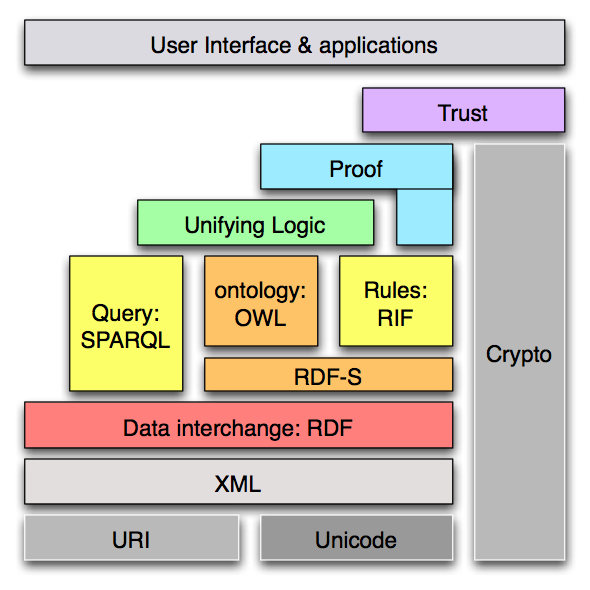
\includegraphics[width=.5\textwidth]{fig/semwebstack}
  \caption{The semantic web architecture}
  \captionsetup{font={footnotesize,bf,it}}
  \caption*{source: \url{http://www.w3.org/2006/Talks/1023-sb-W3CTechSemWeb/\#(19)}}
  \label{fig:semwebstack}
\end{figure} 

\subsection{Introduction to RDF}

RDF provides a framework for representing information which can be exchanged between application without loss of meaning and it is intended for situation in which this information needs to be processed by machines instead of displayed to humans, thus making it fitting for the goals of The Semantic Web  \cite{rdfprimer11}.

This framework has several uses, such as:

\begin{itemize}
	\item Adding machine readable information to web pages, enabling them to be displayed in enhanced formats or to be processed by other agents.
	\item Enriching a database by linking it to third party datasets.
	\item Interlinking API feeds, so that clients can easily discover how to access more information.
	\item Using datasets labeled as Linked Data to build aggregations of data around specific topics or concepts.
\end{itemize} 

RDF information is stored in triples which follow a simple subject-predicate-object pattern. One example of RDF triples which represent knowledge about a person named Bob can be found in listing \ref{lst:bobtriples}. Note that in this set of triples, most attributes appear between brackets, these are International Resource Identifiers (IRIs) linking to other resources, while the other attributes are just literal values. 

\begin{listing}\centering
  \begin{minipage}{.4\textwidth}
    \begin{minted}[linenos=true,mathescape,gobble=6]{xml}
     <Bob> <is_named> "Bob"
     <Bob> <is_a> <Person>
     <Bob> <is_a> <Student>
     <Bob> <knows> <Alice>
     <Bob> <is_interested_in> <Computer_Science>
    \end{minted}
  \end{minipage}
  \caption{Set of triples in pseudocode representing Bob.}\label{lst:bobtriples}
\end{listing}

These IRIs are identifiers for resources on the Semantic Web. Up to now the concepts of URI and IRI have been mixed, to make it clear, an IRI is a generalization of an URI. The form of a IRI is similar to that of the Uniform Resource Locators (URL) used in the World Wide Web, in fact these last are just a form of IRI, thus they look like the following:  \url{http://dbpedia.org/resource/Leonardo_da_Vinci}
 

\subsection{Introduction to Ontologies}

In the Semantic Web, vocabularies or ontologies define the concepts and relationships used to describe and represent a certain area of knowledge, they define the terms that can be used on a application, the possible relationships and their constraints. They are used to help data integration when ambiguity may exist between terms in different datasets, or simply to organize knowledge \cite{w3contologies}.

According to Tom Grubber \cite{gruber1993ontology} An ontology is a formal specification of a shared conceptualization. The concept of Ontology comes from the field of philosophy, however they have been adopted into Artificial Intelligence and Knowledge Representation \cite{chandrasekaran1999ontologies}. Since ontologies are used to create conceptual structure on a domain, they can be used by software for problem solving and reasoning among other tasks.

We can find three types of ontologies:

\begin{description}
	\item[Top-level ontologies]: Describe very general notions which are independant of a particular domain and are applicable to different areas, for example; time, space, events, etc.
	
	\item[Domain ontologies]: The knowledge represented in these ontologies is particular to a certain field of knowledge, such as computers, persons, forestry, etc.	They provide information about concepts in the domain and about the theories governing the domain.
	
	\item[Application ontologies]: This is the least general type of ontology. It describes knowledge specific to a certain a application or task, due to this, they are useful for problem solving.
\end{description}

\section{Introduction to GIS systems}

A Geographical Information System (GIS) integrates hardware, software and data for capturing, managing and displaying all forms of geographically referenced information \cite{esrigis} A GIS provides a framework for gathering and organizing spatial data and related information so it can be displayed and analyzed.

Data on such a system is a digital representation of real world objects. Since this kind of data can be divided into two abstractions, discrete objects (a house, a park) or continuous fields (elevation), two methods are used to store data of this abstractions: Raster and Vector. \cite{giswikigis}

\subsection*{Raster}

Raster data types consist of rows and columns of cells each of them storing a single value, in the say way that a image is composed by pixels. In fact, a Raster data type is, in essence, a type of digital image represented in grids. On a Raster Image each pixels stores a color value which represents certain data, for example, the amount of rain in that region.

This kind of data may be stored in different ways, for example, as a regular .JPEG image or directly in a relational database.

\subsection*{Vector}

Vector data is used to express geographical features, which are represented as geometrical shapes of different types.

\begin{itemize}
	\item \emph{Points:} They are used to describe features that can be represented with a single point, that is, the simplest of features, for example, the location of a monument, the peak of a mountain, etc.
	\item \emph{Lines or polylines:} They are used to represent linear features, such as rivers, roads, trails, etc. It is possible to measure distance on line features.
	\item \emph{Polygons:} They are used for the representation of features that cover a particular area of the earth's surface, for example, a country. It is possible to measure area and perimeter of polygons.
\end{itemize}











\chapter{Project Goals}\label{ch:goals}

\section{Overview}

An overview of the project goal definition document is presented below. The different sections which compose it are the following:

\begin{itemize}
\item \textbf{Project definition:} Statement of the goals of the project, specification of its functional aspects and scope.
\item \textbf{Final product:} Description of the products that are to be developed on the project.
\item \textbf{Project realization:} Definition of the different activities to be carried out in order to fulfill the goals of the project.
\item \textbf{Organization and team:} Description of the Work Team that will carry out the project, as well as its organizational structure and human resources plan.
\item \textbf{Execution conditions:} Project related work conditions, definition of the criteria over which product reception as well as the Change Control.
\item \textbf{Planning:} Establishing of the phases and tasks needed to carry the project, together with orientative dates for their realization.
\item \textbf{Project budget:} Determination of the budget of the project and the associate costs.
\end{itemize}

\section{Project definition}

\subsection{Goals}

The main goal of this project is the combination of geospatial and semantic technologies to build a location aware service based on linked data principles.

The main purpose of the service is to provide the users the capacity to share their knowledge in form of routes and points of interest and to enrich the information obtained using data from the web. Then the generated knowledge can be used to recommend the users new routes or points of interests based on their location and preferences.

The knowledge obtained on the system will be published following the Linked Open Data best practices, so that it can be used by other developers or interested groups.

In addition, it will be possible to obtain an objective difficulty rating for the routes or trails that the users share in the system, relieving from the users the problem of rating their own routes and eliminating possible subjective interpretations.

Together with this, several other services will be provided, allowing users to follow trails from others, to post notes at certain location and to obtain in any moment information regarding their surroundings; all in order to build a GPS community around this service.

So, in short, the goals of the project can be stated in the following way:

\begin{itemize}
\item To build a semantic location-aware service
\item To publish the data of the system following the pattern of Linked Open Data
\item To create a model for the semantic representation of trails and points of interest
\item To build a service that allows the correction and evaluation of a route
\item To build a GPS community based on the location-aware service
\end{itemize}

\subsection{Scope of the project}

In order to fulfill the stated goals, a GIS system based on semantic data will be built. The scope of the project is limited to the following:

\begin{itemize}
\item Research over the areas, technologies and standards that the project touches.
\item Design of a model for the semantic representation of trails and points of interest and a infrastructure that uses and supports this model.
\item Development of a service that makes use of the researched technologies and standards and that follows the previously created design.
\end{itemize}

\subsubsection*{Scope of the research}

Research will be carried over several topics, listed below in order of relevance:

\begin{itemize}
\item The Semantic Web
\item Linked Open Data
\item GIS
\item GPS devices
\item Geographic information standards
\item Development tools and platforms
\item Similar systems
\end{itemize}

\subsubsection*{Scope of the development}

The design and development will cover the following issues:

\begin{itemize}
\item Design and creation of a semantic ontology
\item Development of a location aware web service 
\item Creation of a web application to access the service
\item Development of a mobile application to complement the web
\item Extraction of data from third party sources on the web 
\end{itemize}

\section{Final product}

The project will result in a GIS system which relies on a semantic back end, that is, it stores the data on RDF format and is able to reason over it. The system will be composed by a server, a web client and a mobile application.

This section describes the characteristics of the products that will compose the system.

\subsection{Server}

The server will be formed by two main components, a semantic data store and a web server. The web server will expose the a endpoint that allows direct read-only access to the database, so that other developers are able to query it. In addition, the server will have a NoSQL database used to store sensible information about the users of the system, with the purpose of providing secure authentication.

\subsubsection*{Semantic data store}

The main function of this component will be the storage of the information existing on the system. Since semantic databases - called triplestore because they store the data using a data structure called triples - use ontology oriented data modeling (see section \ref{sec:owl}), the knowledge kept will not belong solely to domain related data, but will also include a ontology that represents the schema of the database and the relations among the resources.

This data store will be accessed through the HTTP protocol, even locally. In fact, it will be possible to query the data base through a read-only endpoint, accessible using HTTP. This way, any developer will be able to use the data in their application directly, without having to follow any predetermined access functions.

Besides, the component will be complemented by a reasoner. This reasoner will be able to infer new knowledge from the existing one. In this context, this means that it will be able to analyze the statements in the database and using the ontology as a basis it will be able to produce new statements.

In addition to regular reasoning, it will also be possible to reason spatially over the data. This way, it will be possible to use the spatial representations of resources in the system to make spatial queries, based on distance and geometric relations.

\subsubsection*{Web server}

The web server is the component that will contain most of the functionality of the server. First, it will implement most of the functions encountered in typical web systems, including user authentication, media upload and read, create and modify operations. All these functions will be exposed through a API, following the REST style.

In addition to these basic functionality, the server will also be in charge of receiving the information about trails and points of interest and analyzing it to obtain additional data. This includes applying a mathematical method to calculate a difficulty score for trails.

The API will also expose function allowing spatial queries without any need of previous knowledge or expertise on this area. For example, a function will allow asking for all the points of interest at a certain distance from another feature. This queries will be limited to retrieval of routes, points of interest and geolocated notes.

The spatial information that the API provides will be exposed following the GeoJSON format.

The server will communicate with the data store using an HTTP interface and sending SPARQL queries for managing the data. In addition to this, the server will carry the task of analyzing the profile of each user and recommending routes that can interest them.

In addition to the mentioned functionality, the server will also expose a HTML5 web socket based API that the mobile application will use to provide real time services to the users.

\subsection{Web application}

The web application will be the main interface through which the users will be able to access the service. The web application will be developed taking into account that it will have to be visualized correctly in all kind of devices and that minimum loading times are desired.

The client will allow users to upload routes and points of interest from GPX files, a standard format for the interchange of GPS information (see section \ref{sec:gpx}). In addition, user will also be allowed to draw the routes on a map or mark the points of interest.

It will be possible to search information about the different features and users of the system, taking advantage of the semantic data, which allows to easily build search engines which go beyond the classic keyword search. The application will offer a detailed view of the data and the possibility to comment on the different user generated features. All this information is to be presented in a easy to read format, that is, using interactive maps to show geographical information.

In addition to all of these, the web will provide a interactive map of the world. Moving and zooming this map will show the different routes and points of interest that the current view of the map covers, this way it will be possible to explore the data on the system without the need of a text search.

A exclusive functionality that the client will offer is a interactive editor. This editor will allow drawing trails and points of interest, providing a way to share knowledge without the need of a file recorded from a GPS. In addition, it will be possible to edit existing routes or trails imported from a file, providing the users with a way of correcting possible GPS generated errors.

The editor will allow the following functions:

\begin{description}
\item[Draw a route on the map:] By repeatedly clicking on the map, specifying the coordinates which form the trail, the users will be able to generate data without a need of GPX files, however, it will be impossible to analyze this trails due to the lack of altitude data.

\item[Mark a point of interest in the map:] With a single click on the map, it will be possible to mark a point of interest in the specified point. The user will be prompted with a form, and by filling it, the point of interest will be uploaded to the server.

\item[Edit a existing route:] Whether it is downloaded from the platform or imported from a file, it will be possible to edit the coordinates of a route by dragging the points that form it.

\item[Fusing two routes:] It will be possible to join the end of a route with the start of another to create a new route.
\end{description}

\subsection{Mobile application}

The mobile application will provide the users with a mean of viewing and browsing though the data on the system, in a similar manner to the web client. However, many of the functions present on the browser base client, for example the editor, will no be present on the mobile client, for the web application will be designed to be usable in mobile browsers.

In addition to the basic functionality, this component will allow the users to record their own trail as they traverse it using the GPS on the mobile device. It will be possible to upload this record to the server or to export it as a GPX or GeoJSON.

The application will also provide a function that allows user to receive real time notifications about the nearby points of interest and geolocated notes. These features will be filtered according to the user preferences, before notifying the user.

It will also be possible to follow the trails that another user has shared, with the mobile application sending a notification to the person using it every time that he/she deviates to much from the established route and indicating how to correct its trajectory.

Finally, the application will allow the creation of geolocated notes. To do this, the user will simply need to write a text, take a photo or record a video and after specifying some privacy settings, the note will be recorded in the system on the current coordinates of the user.

\section{Project realization}

\subsection{Realization methodology}

The development method to be followed through the project consists on a prototype based iterative development methodology. This procedure allow to develop a project splitting it into different phases and developing a functional part of the project at each phase. Figure \ref{fig:iterative} shows a graphical conceptualization of this development methodology.

\begin{figure}[ht]
  \centering
  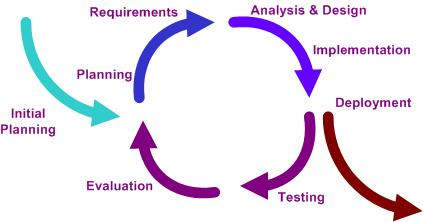
\includegraphics[width=.8\textwidth]{fig/iterative}
  \caption{Iterative development phases}
  \captionsetup{font={footnotesize,bf,it}}
  \caption*{source: \url{http://www.wikipedia.org/}}
  \label{fig:iterative}
\end{figure} 

Thanks to this working methodology, it should be possible to develop independently every components that forms the system and it will be possible to realize effective unit testing over these components.

The development of the project has been split into six phases, whose tasks are listed below. A Work breakdown structure containing the tasks of the project can be found in figure \ref{fig:wbs}.

\subsubsection*{Project opening}
 
This phase consists on the start, organization and planning of the project. The tasks on this phase are not directly related to the development of the final product, yet they are necessary for the development of the project. The tasks in this phase are the following:

\begin{description}
\item[T1.1] Planning and organization

The resources necessary for the realization of the project will be determined and the tasks needed to carry it out will be organized. The development of the project through time will be established.

\item[T1.2] Monitoring

This task will be carried through the whole project. The current status of the project will be monitored to determine the possible existing issues and to ensure that the goals are being reached.
\end{description}

\subsubsection*{Initial research}

The research related with the areas that the project touches will be carried out. The goal of the phase is to obtain the sufficient information to develop a efficient and valid system.

\begin{description}
\item[T2.1] Research on the Semantic Web and Linked Open Data

Research will be done on topics and technologies related to the Semantic Web and Linked Open Data. Other topics will also be investigated, for instance, the representation of spatial data using RDF.

\item[T2.2] Research on technologies

GIS systems, and web and application development tools will be investigated with the goal of establishing an adequate development environment for the project.

\item[T2.3] Analysis of standards and similar system

Existing standards for trail and point of interest representation will be analyzed, as well as the use of this on other platforms and the functionality that similar services offer.

\end{description}

\subsubsection*{Base system development}

The design of the architecture of the system and the development of the software that will be present on the server will be done in this phase. The tasks consist mostly on design, coding and testing.

\begin{description}
\item[T3.1] System design

The technological architecture of the system and of its components will be designed.

\item[T3.2] Test design

The tests to be carried on every component will be determined.

\item[T3.3] Database installation and testing

The semantic database will be installed and tested to guarantee that the desired functionality is granted.

\item[T3.4] Web server implementation and testing

The basic functionality of the web server and related software will be developed and tested. An example of these additional software pieces is the data store connector.

\item[T3.5] API implementation and testing

The functions that the API of the web server exposed will be developed and tested.

\end{description}

\subsubsection*{Web application development}

The web application will be developed using the server produced on the previous phase. Tasks involve mainly interface design, web development and testing.

\begin{description}
\item[T4.1] Interface design

The design of the web interface will be done and the needed resources, such as images and fonts, will be obtained.

\item[T4.2] Implementation and testing

The logic on the web application will be coded and test will be carried out over the developed functions.

\item[T4.3] Editor implementation and testing

The functionality regarding the map editor will be developed and tested.
\end{description}

\subsubsection*{Mobile application development}

The mobile application will be developed using the API of the produced server . Tasks involve mainly interface design, HTML5 development and testing.

\begin{description}
\item[T5.1] Interface design

The design of the mobile interface will be done and the needed resources, such as images and fonts, will be obtained.

\item[T5.2] Implementation and testing

The logic on the mobile application will be coded and test will be carried out over the developed functions.

\end{description}

\subsubsection*{Project finalization}

The last phase will take care of the tasks related to project closure and deployment.

\begin{description}
\item[T6.1] System deployment

The web server will be deployed to a accessible URL and the mobile application will be published on the corresponding markets.

\item[T6.2] Project closure

A final check of the completed goals will be done, future lines of work and possible upgrades will be established and the project will be closed.
\end{description}

\begin{figure}[ht]
  \centering
  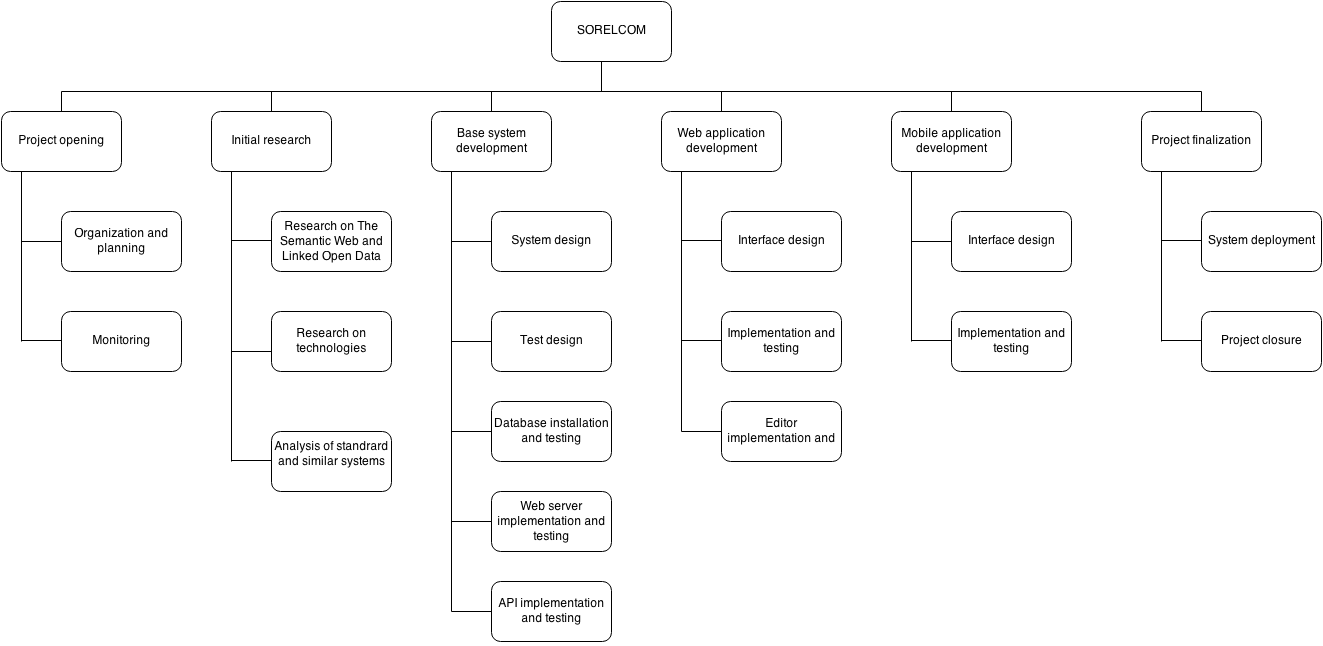
\includegraphics[angle=270, width=.5\textwidth]{fig/wbs}
  \caption{Work breakdown structure}
  \captionsetup{font={footnotesize,bf,it}}
  \label{fig:wbs}
\end{figure} 

\subsection{Intermediate products}

The project is divided on several phases. An intermediate product is obtained from each of the phases or tasks. Table \ref{tab:intermediate-products} offers a reference of the intermediate products of the project and the tasks or phases they relate to.

\begin{table}[ht]
  \centering
  \caption{Intermediate products of the project.}\label{tab:intermediate-products}
  \begin{tabular}{lll}
    \toprule
      \textbf{Name} & \emph{phase}  & \emph{task code}\\
    \midrule
      Technological research & 2. Initial research & T1.1, T1.2 \\
      Ontology specification & 3. Base system development & T3.1 \\
      System architecture & 3. Base system development & T3.1 \\
      Design of the web server & 3. Base system development & T3.1 \\
      Design of the web application & 3. Base system development & T3.1 \\
      Design of the mobile application & 3. Base system development & T3.1 \\
      Test suit & 3. Base system development & T3.2 \\
      Design of the web application interface & 4. Web application development & T4.1 \\
      Design of the mobile application interface & 5. Mobile application development & T5.1 \\
    \bottomrule
  \end{tabular}
\end{table}

These intermediate products are all documents, their contents are listed below:

\begin{description}
\item[Technological research:] Contains a list and of the main technologies that will be involved in the project and a description for each of them.
\item[Ontology specification:] Describes the classes, properties and relations that will appear on the ontology and how they are used to model the data on the system.
\item[System architecture:] Defines which are the components that form the system and how they are related among them.
\item[Design of the web server:] Describes the logical architecture of the web server.
\item[Design of the web application:] Describes the logical architecture of the web application.
\item[Design of the mobile application:] Describes the logical architecture of the mobile application.
\item[Test suite:] Describes the tests to be carried on each of the components of the system.
\item[Design of the web application interface:] Describes the appearance of the web interface.
\item[Design of the mobile application interface:] Describes the appearance of the mobile interface.
\end{description}

\section{Organization and team}

\subsection{Organizational structure}

The organizational structure is relatively simple. The organization involves two main groups, the project manager and the work team.

The project manager is the one in charge of the organization of the project and his function is the direction of the work to do. It takes care of the monitoring and planning of the work as well as most of the validations.

The work group carries out the tasks related to the development of the products of the project. This tasks require research, designs, testing and implementation. The work group will be formed by a single student performing all the required roles.

The organizational schema including all the roles on the project is presented in figure \ref{fig:organization}.

\begin{figure}[ht]
  \centering
  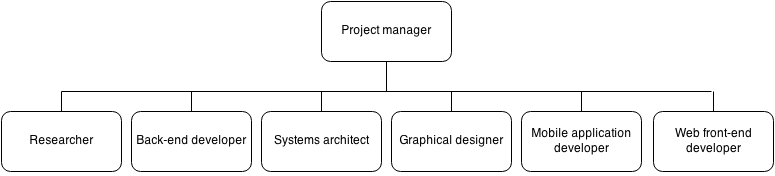
\includegraphics[width=.7\textwidth]{fig/organization}
  \caption{Organizational structure}
  \captionsetup{font={footnotesize,bf,it}}
  \label{fig:organization}
\end{figure} 

\subsection{Human resources plan}

The organization will be formed by the following profiles, each related to the different areas of competence that this project comprises.

\subsubsection*{Project manager}

The project manager is the person in charge of the opening, organization, monitoring and closure of the project. In addition, it is the person in charge of communicating with the management team.

The skills of the project manager should include at least the following:

\begin{itemize}
\item Planning
\item Organizing
\item Communication
\end{itemize}

In addition, it is convenient for it to have knowledge on the areas that the project touches.

\subsubsection*{Researcher}

Due to the innovative nature of the project and the amount of work related to the semantic web, the profile of a researcher is required. The researches takes care of investigating the current state in the areas that the project touches and elaborating state of the art documents needed for the development of the project.

The researcher needs to have knowledge on the areas related to the project, that is, The Semantic Web and Linked Open Data. Learning and writing capabilities are also convenient.

\subsubsection*{Back-end developer}

This profile takes care of developing the back-end of the application, the web server. Due to the nature of its work and the technologies to be used in the project, the following knowledge is required.

\begin{itemize}
\item JavaScript programming skills
\item Knowledge of the NodeJS programming environment
\item Knowledge of the SPARQL query language
\end{itemize}

\subsubsection*{Front-end web developer}

The web developer takes care of creating the web application. Its work involves development of web based graphical user interfaces, due to this and the technologies chosen for the project, the following skills are required.

\begin{itemize}
\item HTML5, CSS3 and JavaScript
\item The AngularJS web development framework
\item The CSS framework Twitter Bootstrap
\item The JavaScript map development library Leaflet
\end{itemize}

\subsubsection*{Mobile application developer}

This profile takes care of developing the mobile application. Proficiency on mobile application programming is needed, however, it is also necessary to know how to use HTML5 native development tools. The required skills can be summarized in the following:

\begin{itemize}
\item HTML5, CSS3 and JavaScript
\item The HTML5 web sockets protocol
\item The HTML5 native mobile development library Phonegap
\item The JavaScript map development library Leaflet
\end{itemize}

\subsubsection{Graphical designer}

The graphics designer takes care of designing the interface of the application. In order to present this design it is required that the designer knows how to use some graphic design tool such as GIMP or Photoshop. 

\subsubsection{Systems architect}

The systems architect takes care of designing the system architecture and the logical design of each component. It should have the following skills:

\begin{itemize}
\item Software design
\item The modeling standard UML
\end{itemize}

\section{Execution conditions}

The usual workplace will be the DeustoTech office located in the 4th floor of the ESIDE building in the university of Deusto. In this environment ethernet network connection is provided as well as a power source for computers. Still, a personal laptop is to be used for the development instead of office computer. Mobile devices used for testing will also be properties of the student.

The weekly schedule is of 18 hours, divided in three hours per day. 

\subsection{Hardware}

Since web and mobile applications are to be developed, there is a need to carry out tests and preview results in various kind of devices, such as mobile phones and tablets. The hardware that is available is the following:

\begin{itemize}
\item Laptop computer, Inter i7 processor, 15 inch screen
\item Android Smartphone, Nexus 5 model
\item iPad tablet
\end{itemize}

\subsection{Software}

The software tools to be used in the project will be open source in most cases, and just free in the rest. In this section the software that is available is listed:

\subsubsection*{Programming tools}

\begin{itemize}
\item NodeJS 0.10.25 - JavaScript runtime environment
\item NPM 1.3.10 - NodeJS package manager
\item Bower 1.3.3 - JavaScript library management tool
\item Yeoman 1.1.2 - JavaScript project scaffolding tool
\item Express 3.4.3 - NodeJS web development library
\item AngularJs 1.2.11 - JavaScript web application development framework
\item Leaflet 0.7.3 - JavaScript map developing library
\item Twitter Bootstrap 3 - CSS responsive web development framework
\item SASS 3.3.8 - CSS development framework
\item Phonegap 2.9.1 - Mobile HTML5 programming platform
\end{itemize}

\subsubsection*{Web browsers}

\begin{itemize}
\item Google Chrome 27 
\item Mozilla Firefox 22
\item Safari 6
\item Opera 12
\item Internet Explorer 10
\end{itemize}

\subsubsection*{Others}

\begin{itemize}
\item Ubuntu 14.04 - Open source desktop operating system
\item Atom 0.105 - JavaScript based code editor
\item Parliament 2.6 - Semantic spatial database, reasoner and endpoint
\item GIT 2.0.0 - Version control system
\item GIMP 2.8 - Image manipulation program
\end{itemize}

\subsection{Change control}

The changing requirements or petitions will follow the proceeding described below:

\begin{enumerate}
\item The change will be communicated to the work group, in case it comes from outside stakeholders.
\item The work group will study the request and evaluate the impact of the potential change in the project.
\item The work group will produce a report that will be sent to the project manager.
\item The project manager will take the final decision on whether to accept the changes or not.
\end{enumerate}

\subsection{Product reception}

During this project two types of product will be created, documents and software. Both of them will be accepted following different procedures.

The documents will follow a previously determined structure. This structure requires each document to have a index, a figure and table index and a list of references used. There is only one requirement regarding the content, documents must start with a overview of the contents of the paper. The author and title of the document must appear at the beginning.

These documents will be sent to the project manager, who will have to accept it in a period of 5 working days. In case of a lack of response, the work team will assume that the document has been accepted so that the development of the project is not stopped.

The software on the other side will follow more rigorous criteria. On the task \textbf{SYS2}, a document specifying the test suite for each component will be created. Software components will only be accepted when they have passes all the specified tests.

\newpage
\FloatBarrier
\section{Planning}

This section presents several aspects related to the project planning. The planning considers a work schedule of 3 hours each day. The project starts Monday 3 of march 2014 and will end the 10th of July of the same year.

\subsection*{Workload estimation per profile}

The estimated work to be done by each profile is shown on this section. 

Table \ref{tab:manager} contains the work to be done by the project manager.

\begin{table}[ht]
  \centering
  \caption{Workload estimation for the project manager.}\label{tab:manager}
  \begin{tabular}{ll}
    \toprule
      \textbf{Task} & \emph{hours}\\
    \midrule
      T1.1 & 6\\
      T1.2 & 16\\
      T6.2 & 3\\
    \bottomrule
      \textbf{Total} & 25\\
  \end{tabular}
\end{table}

Table \ref{tab:architect} contains the work to be done by the system architect.

\begin{table}[ht]
  \centering
  \caption{Workload estimation for the system architect.}\label{tab:architect}
  \begin{tabular}{ll}
    \toprule
      \textbf{Task} & \emph{hours}\\
    \midrule
      T3.1 & 45\\
      T3.2 & 6\\
    \bottomrule
      \textbf{Total} & 51\\
  \end{tabular}
\end{table}

Table \ref{tab:researcher} contains the work to be done by the researcher.

\begin{table}[ht]
  \centering
  \caption{Workload estimation for the researcher.}\label{tab:researcher}
  \begin{tabular}{ll}
    \toprule
      \textbf{Task} & \emph{hours}\\
    \midrule
      T2.1 & 15\\
      T2.2 & 12\\
      T2.3 & 15\\
    \bottomrule
      \textbf{Total} & 42\\
  \end{tabular}
\end{table}

Table \ref{tab:backend} contains the work to be done by the back-end developer.

\begin{table}[ht]
  \centering
  \caption{Workload estimation for the back-end developer.}\label{tab:backend}
  \begin{tabular}{ll}
    \toprule
      \textbf{Task} & \emph{hours}\\
    \midrule
      T3.3 & 3\\
      T3.4 & 30\\
      T3.5 & 24\\
      T6.2 & 3\\
    \bottomrule
      \textbf{Total} & 60\\
  \end{tabular}
\end{table}

Table \ref{tab:webdev} contains the work to be done by the front-end web developer.

\begin{table}[ht]
  \centering
  \caption{Workload estimation for the front-end web developer.}\label{tab:webdev}
  \begin{tabular}{ll}
    \toprule
      \textbf{Task} & \emph{hours}\\
    \midrule
      T4.2 & 27\\
      T4.3 & 21\\
    \bottomrule
      \textbf{Total} & 48\\
  \end{tabular}
\end{table}

Table \ref{tab:mobdev} contains the work to be done by the mobile application designer.

\begin{table}[ht]
  \centering
  \caption{Workload estimation for the mobile application developer.}\label{tab:mobdev}
  \begin{tabular}{ll}
    \toprule
      \textbf{Task} & \emph{hours}\\
    \midrule
      T5.2 & 21\\
    \bottomrule
      \textbf{Total} & 21\\
  \end{tabular}
\end{table}

Table \ref{tab:designer} contains the work to be done by the graphics designer.

\begin{table}[ht]
  \centering
  \caption{Workload estimation for the graphics designer.}\label{tab:designer}
  \begin{tabular}{ll}
    \toprule
      \textbf{Task} & \emph{hours}\\
    \midrule
      T4.1 & 12\\
      T5.1 & 9\\
    \bottomrule
      \textbf{Total} & 21\\
  \end{tabular}
\end{table}

\subsection*{Network and Gantt diagram}

Figure \ref{fig:gantt} shows the gantt diagram for the project, which establishes the temporal planning.
Figure \ref{fig:network-diagram} shows the network diagram of the tasks on the project, in order to identify the dependencies among them.

\begin{figure}[ht]
  \centering
  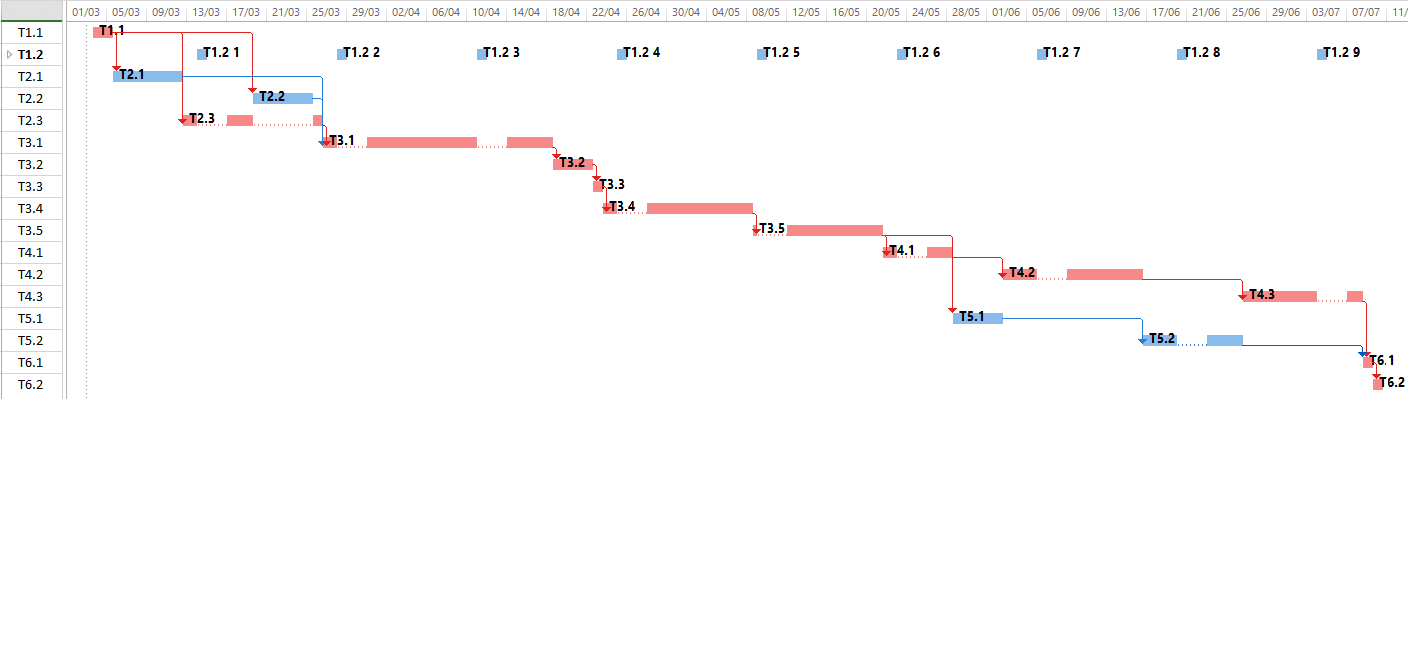
\includegraphics[angle=270,width=.6\textwidth]{fig/gantt-diagram}
  \caption{Gantt diagram}
  \captionsetup{font={footnotesize,bf,it}}
  \label{fig:gantt}
\end{figure} 


\begin{figure}[ht]
  \centering
  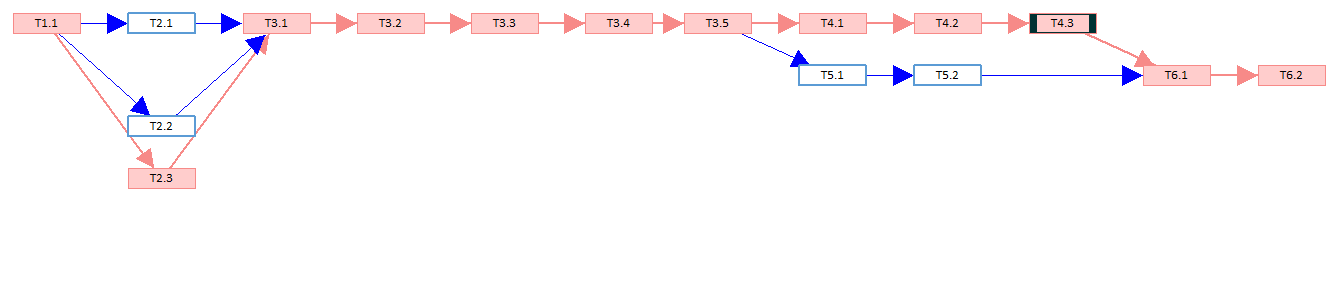
\includegraphics[angle=270, width=.3\textwidth]{fig/network-diagram}
  \caption{Network diagram}
  \captionsetup{font={footnotesize,bf,it}}
  \label{fig:network-diagram}
\end{figure} 

\subsection*{Work plan}

The work plan obtained after establishing the schedule and the interdependencies among tasks is presented in table \ref{tab:project-plan}.

\begin{table}[ht]
  \centering
  \caption{Real work plan.}\label{tab:project-plan}
  \begin{tabular}{llllll}
    \toprule
      \textbf{Identifier} & \emph{start} & \emph{end} & \emph{days} & \emph{profile} & \emph{work (h)}\\
    \midrule
      \textbf{T1 - Project initiation}\\
    \midrule
	  T1.1 & 03/03 & 05/03 & 2 & Project manager & 6\\
      T1.2 & 10/03 & 13/06 & 8 & Project manager & 16\\
    \midrule
      \textbf{T2 - Initial research}\\
    \midrule
      T2.1 & 05/03 & 12/03 & 5 & Researcher & 15\\
      T2.2 & 19/03 & 25/03 & 4 & Researcher & 12\\
      T2.3 & 12/03 & 26/03 & 5 & Researcher & 15\\
    \midrule 
      \textbf{T3 - Base system development}\\
    \midrule
      T3.1 & 26/03 & 18/04 & 15 & System architect & 45\\
      T3.2 & 18/03 & 22/04 & 2 & System architect & 6\\
      T3.3 & 22/04 & 23/04 & 1 & Back-end developer & 3\\
      T3.4 & 23/04 & 08/05 & 10& Back-end developer & 30\\
      T3.5 & 08/05 & 21/05 & 8 & Back-end developer & 24\\
    \midrule
      \textbf{T4 - Web app. development}\\
    \midrule
      T4.1 & 21/05 & 28/05 & 4 & Graphics designer & 12\\
      T4.2 & 02/06 & 16/06 & 9 & Front-end developer & 27\\
      T4.3 & 26/06 & 08/07 & 7 & Front-end developer & 21\\
    \midrule
      \textbf{T5 - Mobile app. development}\\
    \midrule
      T5.1 & 28/05 & 02/06 & 3 & Graphics designer & 9\\
      T5.2 & 16/06 & 26/06 & 7 & Mobile app developer & 21\\
    \midrule
      \textbf{T6 - Project finalization}\\
    \midrule
      T6.1 & 08/07 & 09/07 & 1 & Back-end developer & 3\\
      T6.2 & 09/07 & 10/07 & 1 & Project manager & 3\\
  \end{tabular}
\end{table}

\newpage
\FloatBarrier
\section{Project budget}

The costs associated with the project are divided into two main sources. The first group is the hardware related costs, which comprises the budget required for the physical technological resources used in the realization of the project. Table \ref{tab:hardware} reflects these costs.

The second cost it the one destined to the human resources team. An overview of the costs generated by each profile may be found in table \ref{tab:hhrr}.

No budget will be destined to cover software cost, for the tools used on the project will all be either open source or free-ware. A summary of the project budget can be found in table \ref{tab:budget}.

\begin{table}[ht]
  \centering
  \caption{Hardware related budget.}\label{tab:hardware}
  \begin{tabular}{llll}
    \toprule
      \textbf{Name} & \emph{units}  & \emph{unit price (\euro)} & \emph{cost (\euro)}\\
    \midrule
      Laptop computer & 1 & 1000.00 & 1000.00\\
	  Android smart phone & 1 & 450.00 & 450.00\\
	  iOS tablet & 1 & 500.00 & 500.00\\
    \bottomrule
      \textbf{Total} & & & 1950.00\\
  \end{tabular}
\end{table}


\begin{table}[ht]
  \centering
  \caption{Human resources budget.}\label{tab:hhrr}
  \begin{tabular}{llll}
    \toprule
      \textbf{Name} & \emph{work (h)} & \emph{cost (\euro)}\\
    \midrule
      Front-end web developer & 48  & 240.00\\
	  Back-end developer & 60 & 300.00 \\
	  Mobile application programmer & 21 & 105.00\\
	  Graphics designer & 21 & 105.00\\
	  Researcher & 42 & 210.00\\
	  System architect & 51 & 255.00\\
      Project manager & 25 & 125.50\\
    \bottomrule
      \textbf{Total} & & 1340.00\\
  \end{tabular}
\end{table}

\begin{table}[ht]
  \centering
  \caption{Summary of budget.}\label{tab:budget}
  \begin{tabular}{llll}
    \toprule
      \textbf{Name} & \emph{cost (\euro)}\\
    \midrule
	  Hardware & 1950.00\\
      Human resources & 1340.00\\
    \bottomrule
      \textbf{Total} & 3290.00\\
  \end{tabular}
\end{table}
\chapter{Technological Research}\label{cha:research}

\section{Overview}

This chapter presents the results of the initial technological research done to carry out the project. In here, the main technologies used in the project are explained in detail, as well as the benefits of using them and the reasons for doing so.

The most relevant tools and frameworks used on the project are the following:

\begin{itemize}
	\item RDF
	\item OWL
	\item SPARQL
	\item GeoSPARQL
	\item NodeJS
	\item AngularJS
	\item Leaflet
	\item Phonegap
	\item GPX
	\item GeoJSON
\end{itemize}

There are many other software tools and libraries are used through the project, however, only the most relevant of them, and the ones on which the initial investigation has been carried are shown in this chapter. The rest of the tools are briefly described in chapters \ref{ch:design}, \ref{ch:implementation} and \ref{ch:testing}.

\section{RDF}\label{sec:rdf}

RDF stands for Resource Description Framework, and it is a framework for expressing information about resources. These resources can be anything, documents, people, physical objects, even abstract concepts.

RDF is intended for situation in which data is to be processed by machines and not simply displayed to humans, due to this, it is very useful for the goals of the Semantic Web. It can be used to publish and interlink data on the web. For example, retrieving a resource which represents a person, say Bob, could provide us with the fact that Bob knows another person, say, Alice, who is represented by her URI. Retrieving the resource representing Alice may then yield links to datasets about other persons and so on. A computer can automate this process and follow these links, aggregating data from different resources. This kind of uses are often known as Linked Data \cite{rdfprimer11}. 

There are many reasons to choose using RDF, the following are some of them:

\begin{itemize}
	\item Adding machine readable information to Webpages. This allows them to be displayed in enhanced format or to be processed by roaming agents.
	\item Enriching datasets by linking them to other sources of data.
	\item Interlinking APIs so that clients are able to discover new sources of information.
	\item Using the datasets currently published as Linked Data 
	\item Providing a standards compliant way of exchanging data between applications.
	\item Interlinking various datasets within an organization and allowing cross-dataset queries by using SPARQL.
\end{itemize}

\subsection*{RDF data model}

Data in RDF is formed by statements. This statements are called \textit{triples} and follow a subject-predicate-object structure. A statement on RDF represents a relationship between two resources, the \textbf{subject} and \textbf{object} represent the resources being related while the \textbf{predicate} represents the nature of the relationship. These relationships are phrased in a unidirectional way, from subject to object, and are called properties.

The same subject is often referenced in multiple triples and can of course be the object of other triples. These ability to have the same resource as subject and object in different triples makes it possible to find connections between RDF resources and is one of the most powerful features of the framework. A set of triples can be viewed as a connected \textbf{graph}, in figure \ref{fig:rdfgraph} an example of the visual representation of an RDF graph is given.

\begin{figure}[h]
  \centering
  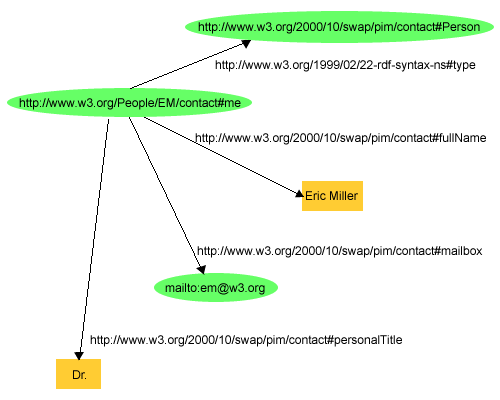
\includegraphics[width=.5\textwidth]{fig/rdfgraph}
  \caption{An RDF graph describing a person}
  \captionsetup{font={footnotesize,bf,it}}
  \caption*{source: \url{http://www.w3.org/TR/2004/REC-rdf-primer-20040210/}}
  \label{fig:rdfgraph}
\end{figure} 

There are three types of RDF data that can occur in triples: IRIs, Literals or Blank nodes \cite{rdfprimer11}.

\subsubsection*{IRIs}

IRI is an abbreviation for International Resource Identifier, which is used to identify a resource. On RDF, IRIs may appear in any component of triples, be it subject, object or predicate. The URLs (Uniform Resource Locators) which identify web pages are a form of IRI, however other forms of IRI can identify a resource without specifying its location. An IRI is a generalization of URIs allowing the use of non-ASCII characters unlike the latter. Thus, an IRI is defined as a set of characters unreserved characters which can include characters of the UCS \cite{rfc3986,rfc3987}(Universal Character Set, [ISO10646]).

An example of a IRI from dbpedia can be the following: \url{http://dbpedia.org/resource/Leonardo_da_Vinci}. Even if RDF does not explicitly specify what a certain IRI represents, they can take meanings from vocabularies or conventions.

In SPARQL (see \ref{sec:sparql}) and in some RDF serialization models prefixes can be defined. A dataset, for example http://example.org, could be given the name \textit{my}. By giving this name we can reference http://example.org/Bob, a resource on the dataset as my:Bob. This is useful for it helps to avoid clutter on the query and helps human understanding, thus, from now on, prefix notation will be used to express datasets and vocabularies on the document.

\subsubsection*{Literals}

Literals are the basic values that are not IRIs. Literals are associated with data types, for example, the \textit{Integer} and \textit{Float} data types are equivalent to the traditional types from the programming languages. The string typed literals may optionally have a language associated allowing internationalization. Most of the regularly used data types are defined by XML Schema \cite{xmlschema}.

One particularity of RDF data types is that they can be defined on ontologies. Due to this, it is possible to find custom types, such as a string representing the serialization in WKT \cite{wkt} format of a geometry. 

An example of different types of triples, including literals can be found in listing \ref{lst:triplesliterals}.

\begin{listing}[ht]\centering
  \begin{minipage}{.6\textwidth}
    \begin{minted}[linenos=true,mathescape,gobble=6]{xml}
      <my:Bob> <foaf:name> "Bob"
      <!--The object is a literal of type String -->
      <my:Bob> <rdf:type> <foaf:Person> 
      <my:Bob> <foaf:age> "19"^^xsd:Integer 
      <!-- The literal is of type Integer -->
    \end{minted}
  \end{minipage}
  \caption{Different types of triple statements.}\label{lst:triplesliterals}
\end{listing}

\subsubsection*{Blank nodes}

Blank nodes are used to refer to resources who don't have or need a global identifier (an IRI). For example, we may want to refer to the right arm of a person, however, we may think that it is too verbose or unnecessary to actually give a identifier to this arm, so we could use a blank node to represent it, as illustrated in listing \ref{lst:triplesblanknode}. In this example it makes sense to have a blank node, for the right arm is directly dependent on the person, an arm (usually) makes no sense detached from a person.

\begin{listing}[ht]\centering
  \begin{minipage}{.6\textwidth}
    \begin{minted}[linenos=true,mathescape,gobble=6]{xml}
      <my:Bob> <rdf:type> <foaf:Person> 
      <my:Bob> <my:hasRightArm> :_b1
      :_b1 <rdf:type> <my:Arm>
    \end{minted}
  \end{minipage}
  \caption{Triple statements with a blank node.}\label{lst:triplesblanknode}
\end{listing}

\subsection*{RDF vocabularies}\label{ssec:rdfvocabularies}

The data model of RDF does not make any assumptions about the meaning of the IRIs representing the resources. However, in the reality, RDF is usually used in conjunction with a series of vocabularies or other conventions that give semantic information about these resources.

Many vocabularies are currently considered standard due to their wide use among Linked Open Data systems. Some of these ontologies are the following.

\begin{description}
	\item{Friend of a Friend (FOAF):} One of the first vocabularies used worldwide, it is used to represent persons, the properties that identify them and the relations among them \cite{foafspec}.
	
	\item{Dublin Core:} A metadata element set for describing a wide range of resources. Contains properties such as the creation date of the resource \cite{dublincorespec}.
	
	\item{schema.org: } A vocabulary for marking up web pages so that search engines can more easily find them \cite{schemaspec}.
\end{description}

\subsection*{RDF schema}

RDF Schema (RDFS) is a extension of RDF. It provides a data-modeling vocabulary for RDF data, in this way, RDFS extends RDF by giving externally specified semantics to specific resources, semantics which cannot be captured in plain RDF \cite{rdfs1}. RDF Schema provides information about interpretation of the statements in a data model, however, it does not constrain the syntactical appearance of RDF descriptions.

The extension provides mechanisms to describe groups of related resources and the relationships between these resources, as well as classification hierarchies. The class and property system that can be expressed is similar to the type systems of object oriented programming, however, instead of defining classes in terms of the properties their instance have, they are defined in terms of classes of resource to which they apply \cite{rdfschema}.

RDF schema is written in plain RDF, thus it takes form of a vocabulary. The classes and properties provided are listed below:

\subsubsection*{Classes}

\begin{description}
\item[\texttt{rdfs:Resource}] All things described by RDF are called resources and are instances of this class. It is the class of everything and all other classes are \textit{subclasses} of it.

\item[\texttt{rdfs:Class}] It is the class of all the resources that are classes, thus, \texttt{rdfs:Class} is an instance of \texttt{rdfs:Class}.

\item[\texttt{rdfs:Literal}] It is the class of literal values such as strings and integers. It is an instance of \texttt{rdfs:Class}.

\item[\texttt{rdfs:Datatype}] It is the class of datatypes, such as \texttt{integer}.

\item[\texttt{rdf:langString}] It is the class of language tagged string values, an instance of \texttt{rdfs:Datatype} and subclass of \texttt{rdfs:Literal}.

\item[\texttt{rdf:HTML}] It is the class of HTML string values, an instance of \texttt{rdfs:Datatype} and subclass of \texttt{rdfs:Literal}.

\item[\texttt{rdf:HTML}] It is the class of HTML string values, an instance of \texttt{rdfs:Datatype} and subclass of \texttt{rdfs:Literal}.

\item[\texttt{rdf:XMLString}] It is the class of XML literal values, an instance of \texttt{rdfs:Datatype} and subclass of \texttt{rdfs:Literal}.

\end{description}

\subsubsection*{Properties}

\begin{description}

\item[\texttt{rdfs:range}] It is used to indicate that the values of a property are instances of a certain class.

\item[\texttt{rdfs:domain}] It is used to indicate that any resource that has the given property is a instance of a certain class.

\item[\texttt{rdfs:type}] It is used to state that a resource is a instance of a certain class.

\item[\texttt{rdfs:subClassOf}] It is used to state that all instances of one class are also instances of another.

\item[\texttt{rdfs:subPropertyOf}] It is used to state that all resources related by a class are also related by another.

\item[\texttt{rdfs:label}] It is used to provide a human readable version of the name of the resource.

\item[\texttt{rdfs:comment}] It is used to provide a human readable description of a resource.

\end{description}

\subsubsection*{Use of RDFS}

RDFS provides with a vocabulary to express relations among RDF resources, which allow for reasoning and inference over datasets. However, this vocabulary is very limited, it does not allow much more that the definition of classification hierarchies. These hierarchies are defined in regular RDF triples, as shown in listing \ref{lst:rdfschema}.

\begin{listing}[ht]\centering
  \begin{minipage}{.6\textwidth}
    \begin{minted}[linenos=true,mathescape,gobble=6]{xml}
      <foaf:Person> <rdf:type> <rdfs:Class> 
      <my:knows> <rdf:type> <rdf:Property>
      <my:knows> <rdfs:domain> <foaf:Person>
      <my:knows> <rdfs:range> <foaf:Person>
      <my:friendOf> <rdfs:subPropertyOf> <my:knows>
    \end{minted}
  \end{minipage}
  \caption{RDFS class and property hierarchy.}\label{lst:rdfschema}
\end{listing}

In addition to ability to express relations, RDFS provides additional constructs for the representation of resources. The vocabulary defines containers, such as bags and sequences, in addition to properties to indicate membership to these. Besides collections, the ontology defines a more sophisticated mechanism for data structuring; RDF lists, which are similar to the Linked List data structure. However, the usage collections bring an additional layer of complexity to the dataset, thus they are scarcely used.

\subsection*{Why RDF?}

Using RDF can greatly benefit this project. It can give a representation of the relationships on the system which can be easily analyses by machines. This can help building important functions, such as the recommendation system.

However, the use of RDF on this project is almost mandatory, for one of the goals is achieving data interoperability and publishing the data as Linked Open Data on the web. Anyway, the expressive level provided by RDF schema is not enough for the needs of the project, so another vocabulary must be used.

\section{OWL}\label{sec:owl}

The Web Ontology Language (OWL) is a semantic markup language for publishing and sharing ontologies in the World Wide Web \cite{bechhofer2009owl}. The language is designed for applications that need to process the content of the information instead of just presenting it to humans. OWL provides greater machine interpretability than RDF or RDF schema by providing additional vocabularies along formal semantics.

OWL is used to explicitly represent the meaning of terms in vocabularies and the relationships among these terms. These representations are called ontologies \cite{mcguinness2004owl}. The standard is part of the stack of W3C recommendations for the semantic web, together with XML, XML Schema, RDF and RDF Schema.

OWL provides three sub-languages with increasing expressive power. Each subset of OWL includes all the previous ones, in addition to RDFS and RDF, so that there is no loss on expressive power as illustrated in figure \ref{fig:owlstack}.

\begin{figure}[h]
  \centering
  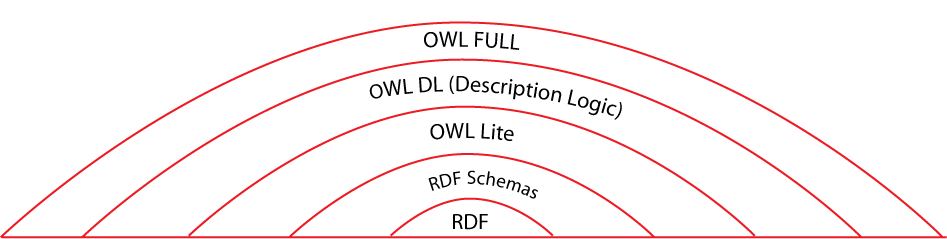
\includegraphics[width=.7\textwidth]{fig/owl-stack}
  \caption{The OWL levels of expressivity}
  \captionsetup{font={footnotesize,bf,it}}
  \caption*{source: \url{http://www.w3.org/}}
  \label{fig:owlstack}
\end{figure} 


\subsection*{OWL Lite}

OWL Lite is designed to support those users who need only a classification hierarchy and simple constraints. For example, while supporting cardinality constraints, it only allows cardinality 0 or 1, for the sake of simplicity. Due to this it should be simpler to provide tool support for OWL lite than to its other, more expressive, relatives. It also has a lower level of formal complexity than its more expressive siblings.

This sub-language contains all the features of RDF schema, such as category definitions through classes and hierarchical classification through subclasses, plus additional restrictions and expressions. OWL Lite provides tools for defining equality and inequality relations, property characteristics, property restrictions, restricted cardinalities and class intersections.

\subsubsection*{Equality and Inequality}

They are used to indicate equality and inequality relations among classes. One example

\begin{description}
\item[\texttt{equivalentClass}] Two classes may be stated as equivalents. This equality is used to create synonyms.

\item[\texttt{equivalentProperty}] It is used to define synonymous properties, the same way as with classes.

\item[\texttt{sameAs}] It states that two individuals are the same.

\item[\texttt{differentFrom}] The opposite to \texttt{sameAs}, used to indicate that two individuals are different. 

\item[\texttt{allDifferent}] It can ve used to state that a number of individuals are different from each other.
\end{description}

\subsubsection*{Property characteristics}

Property characteristics are special identifiers in OWL that provide information concerning the properties and their values. These characteristics are placed on properties, with relation to no class, as in listing \ref{lst:owl1}.


\begin{listing}[ht]\centering
  \begin{minipage}{.8\textwidth}
    \begin{minted}[linenos=true,mathescape,gobble=6]{xml}
      <owlx:ObjectProperty owlx:name="adjacentRegion" owlx:symmetric="true">
        <owlx:domain owlx:class="#Region" /> 
        <owlx:range owlx:class="#Region" />
      </owlx:ObjectProperty>
    \end{minted}
  \end{minipage}
  \caption{OWL property characteristic example.}\label{lst:owl1}
\end{listing}


\begin{description}
\item[\texttt{inverseOf}] Describes that a property is inverse to another. If A is related to B by the property P1 and P2 is the inverse of P1, then B will relate to A by property P2.

\item[\texttt{TransitiveProperty}] States that a property is transitive. For example, if A is related by transitive property P to B and B is related by P to C, then A will also be related by P to C.

\item[\texttt{SymmetrycProperty}] If a property is stated to be symmetric, then if A is related to B by the property, B will also by related to A by the same property.

\item{\texttt{FunctionalProperty}} If a property is functional, then it can have no more than one value for each individual. This mean that there will be no two triples of the same individual containing this property as a predicate.

\item[\texttt{InverseFunctionalProperty}] It states that the inverse of a property is a functional property.
\end{description}

\subsubsection*{Property restrictions}

OWL Lite allows to place restrictions regarding on how properties can be used inside of instances of classes. One example can be found in listing \ref{lst:owl2}

\begin{listing}[ht]\centering
  \begin{minipage}{.8\textwidth}
    \begin{minted}[linenos=true,mathescape,gobble=6]{xml}
      <owlx:Class owlx:name="Wine" owlx:complete="false">
        <owlx:Class owlx:name="&food;PotableLiquid" />  
        <owlx:ObjectRestriction owlx:property="#hasMaker"> 
          <owlx:allValuesFrom owlx:class="#Winery" />
        </owlx:ObjectRestriction> 
      </owlx:Class>
    \end{minted}
  \end{minipage}
  \caption{OWL property restriction example.}\label{lst:owl2}
\end{listing}


\begin{description}
\item[\texttt{allValuesFrom}] This restriction is placed on a property in relation to a class. It indicates that a property on a particular class has a local range restriction associated with it. For example, the class \textit{Person} may have a property \textit{hasDaugther}, restricted to have all values from class \textit{Woman}. This means that if an individual of type person is related by a relation \textit{hasDaugther} to other individual, we can infer that this individual will be a woman.

\item[\texttt{someValuesFrom}] This restriction is placed on a property in relation to a class. It indicates that at least one value from the property is of a certain type. For example, the class \textit{SemanticWebPaper} may have a property \textit{hasKeyword} restricted to have some values from \textit{SemanticWebTopic}. This would mean that a semantic web paper can have any number of keywords from any topic, as long as at least one of them belongs to a semantic web topic.
\end{description}

\subsubsection*{Restricted cardinalities}

OWL includes a limited form of cardinality restrictions. These are placed on properties with respect to classes, that is, the restrictions constrain the cardinality of the property in instances of a specific class.

\begin{description}
\item[\texttt{minCardinality}] If a minimum cardinality of 1 is stated on a property with respect to a particular class, then any instance of that class will be related to at least one individual by that property. For example, a person must have some sort of identifying card, thus, a minimum cardinality of 1 should be placed on the relation \textit{hasIDCard} with respect to \textit{Person}.

\item[\texttt{maxCardinality}] If a maximum cardinality of 1 is placed on a property with respect to a particular class, then any instance of that class will be related to at most one individual by that property. For example, a person should have at most one ID card, thus, the relation \textit{hasID} would have a maximum cardinality of 1.

\item[\texttt{cardinality}] It is used as a convenience to indicate that a property has both a maximum and a minimum cardinality with the same values. 
\end{description}

\subsubsection*{Intersection}

OWL Lite offers a very limited expressibility for intersections through the property \texttt{intersectionOf}. With this expression one could express that a \textit{EmployedPerson} is a intersection of a \textit{Employee} and a \textit{Person}. An example for this is shown in listing \ref{lst:owl3}

\begin{listing}[ht]\centering
  \begin{minipage}{.8\textwidth}
    \begin{minted}[linenos=true,mathescape,gobble=6]{xml}
      <owlx:Class owlx:name="WhiteWine" owlx:complete="true">
        <owlx:IntersectionOf>
          <owlx:Class owlx:name="#Wine" />
          <owlx:ObjectRestriction owlx:property="#hasColor">
            <owlx:hasValue owlx:name="#White" /> 
          </owlx:ObjectRestriction>
        </owlx:IntersectionOf>
      </owlx:Class>
    \end{minted}
  \end{minipage}
  \caption{OWL property restriction example.}\label{lst:owl3}
\end{listing}

\subsection*{OWL DL and OWL Full}

OWL DL is the second among the OWL sub-languages. It includes all the expressive power of OWL lite and adds on top of it. Similarly OWL Full adds on top of OWL DL. However, OWL Full is usually deemed as undecidable, in fact, there are no reasoners that can guarantee a solution in finite time. Due to this, many reasoners for OWL DL, such as Pellet try to find a way to convert OWL Full ontologies to a more a previous level of expressivity, since most ontologists use the highest expressive power when they only need OWL DL at most \cite{pellet}.

\subsection*{Why OWL?}

RDF schema provides a very limited way of expressing ontologies, it only allows to build classification hierarchies. Due to this, using OWL to describe the ontology would be the most recommendable thing. More specifically, the expression level of OWL DL, which allows to describe disjoint relations between classes (among other relation) plus all of the OWL Lite characteristics listed above, will allow to build a complete and correct ontology.
\section{SPARQL}\label{sec:sparql}

SPARQL is the recursive acronym for SPARQL Protocol and RDF Query Language. As its name indicates, it is a protocol and query language for RDF data. The idea behind this language is to allow the querying over RDF datasets in a similar language in which triples are expressed \cite{sparqlprotocol}.

SPARQL allows querying \cite{sparqlquery} and updating \cite{sparqlupdate} of RDF datasets. Similar to RDF, this language is composed of triples, however among the subjects predicates and objects, variables can be introduced. The logic behind SPARQL is stating a set of triples and introducing a variable somewhere among these triples. By doing so, the query engine will look and retrieve for all the cases which satisfy the set of triples in the query. Nothing impedes to query for a certain triple without specifying any variable, which can be useful when the goal is to know if the triple actually exists, but it is not the usual case.

In SPARQL prefixes can be used to indicate name spaces. By using the keyword prefix, it is possible to specify a URI which will be prepended to all triples using that resource. Variables are specified by using a interrogation mark (?) before an arbitrary name. Two examples can be found in listings \ref{lst:sparqlbasic} and \ref{lst:sparqlmedium}.

\begin{listing}[ht]\centering
  \begin{minipage}{.6\textwidth}
    \begin{minted}[linenos=true,mathescape,gobble=6]{sparql}
      SELECT ?s ?p ?o WHERE {
      	?s ?o ?o .
      }
    \end{minted}
  \end{minipage}
  \caption{SPARQL query for retrieving all triples on the dataset.}\label{lst:sparqlbasic}
\end{listing}

This example is very basic, it does not actually specify any concrete triple it states subject object and predicate as variables. Due to this, the query engine will match every existing statement in the database and will retrieve all triples.

\begin{listing}[ht]\centering
  \begin{minipage}{.7\textwidth}
    \begin{minted}[linenos=true,mathescape,gobble=6]{sparql}
      PREFIX my: <http://example.org>
      PREFIX foaf: <http://xmlns.com/foaf/0.1/>
      PREFIX rdf: <http://www.w3.org/1999/02/22-rdf-syntax-ns#>
      
      SELECT ?name WHERE {
      	?person rdf:type foaf:Person .
      	?person foaf:name ?name .
      }
    \end{minted}
  \end{minipage}
  \caption{SPARQL query for retrieving names on the dataset.}\label{lst:sparqlmedium}
\end{listing}

This case is slightly more elaborated than the previous one. First the keyword PREFIX appears, which specifies namespaces for the query, similar to how XML namespaces work. After the prefix declaration, there is a SELECT keyword. Here the operation to be done is specified, among the options of SELECT for regular queries, ASK for boolean queries, INSERT for data insertion and DELETE for data removal. After the select, the variables to be retrieved, bound in SPARQL terms, are specified. After that, the actual triples of the query are written. In this case a \textit{person} variable is used to retrieve every resource of type \textit{Person} in the dataset. Then if that resource contains a name, it is bound to the variable.

It is possible to use more advanced operations in SPARQL. Every triple statement is a implicit intersection, however, it is possible to use the keyword UNION as well. It is also possible to count the amount of occurrences of a variable, to order by variable values and even to filter with regular expressions. Utilities for retrieving only a certain subset of query matching elements are also provided, allowing to limit the result to a certain amount of triples or event to offset the start of the result to a certain triple.

\subsection*{Why SPARQL?}

Since the system will store data in RDF format, the use of SPARQL as a query language becomes obligatory. Still, there are several benefits for the use of SPARQL over a more traditional language such as SQL or over using a ORM. This protocol is designed for advanced queries, thus it allows to find complex relations among data in a relatively easy manner. 

Besides, since SPARQL is a standard language, the same queries used for the system could be used to retrieve data from external datasets.

\section{GeoSPARQL}\label{sec:geosparql}

RDF and SPARQL allow for reasoning in a large domain of applications, however, these reasoning is only concerned about relations explicitly represented in the datasets. This does not include the spatial relations we aim to represent in the system, such as nearby relations.

GeoSPARQL is a standard which aims to provide support from representing and querying spatial data over the semantic web. This standard has been presented by the Open Geospatial Consortium (OGC) and is designed modularly \cite{geosparqlspec, battle2012enabling}. The components that form the specification are listed below \cite{battle2011linking}:

\begin{itemize}
	\item A vocabulary to represent spatial features, geometries and their relationships.
	\item A set of domain-specific spatial functions to use in SPARQL queries.
	\item A set of query transformation rules
\end{itemize}

\subsection*{Vocabulary}

The ontology used to represent spatial data is domain independent in the sense that it is only concerned in representing spatial objects and relations, without specifying the type of resources it represents. Thanks to this is can be used to model any kind of GIS system, whether it represents nature, a country's road infrastructure or cultural points of interest.

The ontology provides two type of top-level classes, \textit{Features} and \textit{Geometries}. Features are simply entities in the real world with some spatial location. A feature can have any kind of spatial form that cannot be precisely defined, for example, a lake or a forest. A \textit{Geometry} on the other hand is any geometric shape, such as a point or a polygon used as a representation of the spatial location of a feature.

Together with these types, a medium for representing the exact geometries of the object is provided. By using the properties \textit{asWKT} and \textit{asGML} it is possible to provide the exact spatial information as a WKT or GML \cite{gmlspec} string, as in the listing \ref{lst:geosparql1}.

\begin{listing}[ht]\centering
  \begin{minipage}{.6\textwidth}
    \begin{minted}[linenos=true,mathescape,gobble=6]{xml}
      <my:Point> <rdf:type> <geo:Feature> 
      <my:Point> <geo:hasGeometry> <my:geom>
      <my:geom> <rdf:type> <geo:Geometry>
      <my:geom> <geo:asWKT> "POINT(0, 0)"^^geo:wktLiteral
    \end{minted}
  \end{minipage}
  \caption{A feature in the GeoSPARQL vocabulary.}\label{lst:geosparql1}
\end{listing}

Besides, there is also a way to provide represent non-exact relation, using qualitative properties, such as the \textit{within} property.

\subsection*{SPARQL extension}

Exploiting the qualitative relations in the system is simple, a regular query can be used. However, in order to take advantage of the serialization of geometries, GeoSPARQL defines a series of functions that allow the manipulation and querying of spatial data. For example, the function \textit{geof:distance} will return the shortest distance between two geometries.

This way, a extension for SPARQL is provided, which allows to find the implicit spatial relations in the dataset, as in the query shown in listing \ref{lst:geosparql2}

\begin{listing}[ht]\centering
  \begin{minipage}{.6\textwidth}
    \begin{minted}[linenos=true,mathescape,gobble=6]{sparql}
      SELECT ?p
      WHERE {
        ?p a geo:Feature
        ?p geo:hasGeometry ?pgeo .
        ?pgeo geo:asWKT ?pwkt .
        ?w a geo:Feature .
        ?w a my:Park .
        ?w geo:hasGeometry ?wgeo .
        ?wgeo geo:asWKT ?wwkt .
        FILTER(geof:distance(?pwkt ?wwkt units:m)
          < 3000)
      }
    \end{minted}
  \end{minipage}
  \caption{Spatial query in SPARQL.}\label{lst:geosparql2}
\end{listing}

\subsection*{Why GeoSPARQL?}

While there are some semantic storage systems that implement their own spatial indexes and representation system there has been no standard in the semantic web until the appearing of GeoSPARQL. 

However due to the innovative character of this standard, there are few systems which actually implement it. Anyway, the usage of this protocol in the system will benefit the system, for in the future, if the standard is adopted worldwide, the data will be more fitting to the Semantic Web.

\subsubsection*{Parliament}

Parliament\texttrademark \cite{parliament} is a triple-store, SPARQL endpoint and reasoner created by SemWebCentral in 2009. It is one of the few existing semantic databases which support the GeoSPARQL protocol, and it does so without then need of a relational spatial database on the back-end. 

Parliament provides a SPARQL endpoint over which selection or update queries can be done. Besides it provides a reasoner which allows to make spatial queries. This database-reasoner-endpoint bundle makes this software very adequate to support the semantic GIS system to be produced. In addition, the reasoner that the bundle provides supports OWL lite, thus it is not necessary to use any additional software to reason over the data. 

\section{NodeJS}\label{sec:node}

NodeJs is a framework based on Chrome's runtime engine \cite{v8} for developing high-performance, concurrent programs that instead of relying on the mainstream multi-threading approach use asynchronous I/O \cite{tilkov2010node}.

The reason behind the development of this framework is mainly that Thread-Based networking is inefficient and difficult to use. Node will be much more memory efficient under high load that systems which allocate threads for each connection.

Node differs from other frameworks such as Django or Rails in that it uses a event driven programming model. In Node, the event model is taken further that in the rest of frameworks, the event loop is presented as a language construct instead of a library. In other languages the event loop is typically started through a blocking call such as \texttt{EventMachine.run()} however, in Node, there is no event loop start call, it simply enters it after executing the input script and exits it when there are no more callbacks to execute.

One example of Node's programming model is shown in listing \ref{lst:node1}. In the example, a web server listening on port 1337 is created. To when creating this server a callback is passed; every time a connection is made the web server responds with a "Hello world". The process will tell the operating systems to notify it when a new connection is made, and then go to sleep. When new connections are made the callback will be executed, each connection is just a small memory allocation.

\begin{listing}[ht]\centering
  \begin{minipage}{.6\textwidth}
    \begin{minted}[linenos=true,mathescape,gobble=6]{javascript}
	     var http = require('http');
	     http.createServer(function (req, res) {
	       res.writeHead(200, {'Content-Type': 'text/plain'});
	       res.end('Hello World\n');
	     }).listen(1337, "127.0.0.1");
	     console.log('Server running at http://127.0.0.1:1337/');
    \end{minted}
  \end{minipage}
  \caption{NodeJS "hello world" web server.}\label{lst:node1}
\end{listing}

The framework is powered by a module system. Modules make it possible to include other JavaScript files into an application, using the keyword \textit{require} to load them. This functionality allows easy use of external libraries, in fact, most of the core functionality is written using modules.

NodeJS treats HTTP as a first class protocol, attempting to correct most of the problems that arise in other web frameworks such as HTTP streaming. Thanks to this approach, the platform gives a good foundation for creating web development libraries such as Express.

\subsection*{NPM}

NPM stands for Node Package Manager. It is a tool built to allow for easy installation and control of NodeJS modules. The software offers a simple command line interface to work with. In addition, it offers a way of managing node projects by using JSON configuration files.

By creating a file named \textit{package.json}, it is possible to specify the modules used on the project and their version, plus several other configuration options such as a remote repository.

When using Node to build applications it is almost unavoidable to use NPM to install the needed libraries.

\subsection*{Express}

Express is a minimalist and flexible web application development library built on top of NodeJS. It offers a URL routes, template engine utilities and middle ware among other things. 

Express is currently the de facto standard in Node web application development, mainly due to the ease of use it offers. The library offers an \texttt{express} object on which callback functions for different HTTP requests can be registered. These callbacks are provided with a request and response object which can be used to analyse the request made to the server and to respond respestively. The example on listing \ref{lst:node2} creates a express server on port 3000, which will respond to queries on the route "/hello".

\begin{listing}[ht]\centering
  \begin{minipage}{.6\textwidth}
    \begin{minted}[linenos=true,mathescape,gobble=6]{javascript}
	     var express = require('express');
	     var app = express();
	     app.get('/hello', function(req, res){
	       res.send('Hello World');
	     });
	     var server = app.listen(3000, function() {
	      console.log('Listening on port %d', server.address().port);
	     });
    \end{minted}
  \end{minipage}
  \caption{Express "hello world" program.}\label{lst:node2}
\end{listing}

Aside from the basic functionality, the library offers a series of shortcuts for rendering parameterized HTML templates, and for building JSON based APIs.

\subsection*{Why NodeJS}

There are several frameworks which could have been used for this project. Jena, a Java framework for Semantic Web application is typically used to manipulate data, and other frameworks such as Django offer very complete geospatial API. Node offers none of these, however, the advantages on performance and scalability it offers out weight other tools. Besides, the student's previous experience with Node has also been taken into account when choosing Node as the working platform.
 
\section*{AngularJS}\label{sec:angular}

In the last years, there has been a trend to develop web applications instead of developing natively for each operating system. The rise in computational power allows for complex processes to be executed in web browsers and makes the software installation times meaningless, which is causing a shift from native development to web development.

Developing applications for the web has several advantages: there is no need to think in multi-platform development, it is granted; there is no need for installation, etc. Still, there are several issues that arise when developing on the web. The main issue is related to complexity on big JavaScript apps; when projects grow enough it becomes nigh impossible to manage them, due to the lack of structure inherent to most JavaScript projects.

Due to this, tools have been developed to ease web application development. One of the most prominent among these tools is AngularJS, a framework with focus on SPA (Single Page Application) development following the MVC (Model-View-Controller) pattern \cite{angularjs1, angularjs2}.

Angular has been developed with several goals in mind: First, reducing the amount of DOM manipulation on the code, separating the client side of the application from the server side, giving structure to web applications and improving the capability to test the code.

\subsection*{Model View Controller}

The MVC pattern is implemented in this framework by separating the application into three main components \cite{angularjs3}.

\begin{description}
\item[The view:] The HTML templates which can be found in any web page are the view, however, unlike in regular applications, they are extended using directives provided by the framework.
\item[The controller:] Angular allows the definition of controllers in a application. They are used to define operation which will manipulate the data and the views. The views and the controllers are related through an object called \texttt{\$scope} (see figure \ref{fig:angularscope}).
\item[The model:] Any data which belongs to the application domain is considered part of the model. Usually the data is obtained from the server, through REST APIs, since function to easy asynchronous requests are provided.
\end{description}

\begin{figure}[ht]
  \centering
  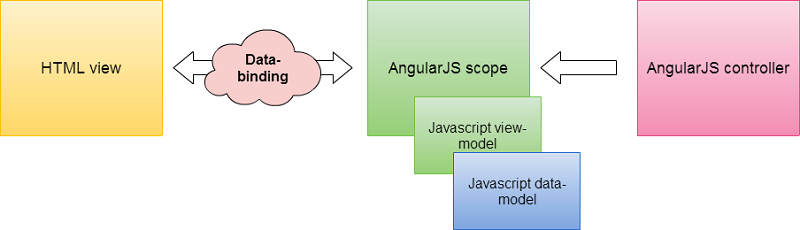
\includegraphics[width=.8\textwidth]{fig/angular-scope}
  \caption{View-controller binding through the scope}
  \captionsetup{font={footnotesize,bf,it}}
  \caption*{source: \url{http://s.codeproject.com/}}
  \label{fig:angularscope}
\end{figure} 

In addition to the mentioned, the framework allows the definition of \textit{Services} and \textit{Directives}. Services are object that can be injected into a controller and have a wide array of uses, from code reusing to data sharing among controllers. Directives on the other side are utilities to manipulate the views and aren  used in the HTML views. One example of such directives is \texttt{ng-click} which is used to specify which operation will be executed when a element on the DOM is clicked.

The MVC in Angular works using a two-way binding. Data is bound to the view through the \texttt{\$scope} object; if a change happens in the view, the data in the models is automatically updated and if a controller modifies the data in the models, the view is automatically updated. An example is shown on listing \ref{lst:angular1}. In this example. when the button is clicked, the function \texttt{change} will be executed, changing the value on the variable \texttt{text} which will automatically update the paragraph on the view.

\begin{listing}[ht]\centering
  \begin{minipage}{.6\textwidth}
    \begin{minted}[linenos=true,mathescape,gobble=6]{html}
	     <div ng-controller="ExampleCtrl">
	       <p>{{text}}</p>
	       <button ng-click="change()"> 
	         Change text 
	       </button>
	     </div>
	     <script type="text/javascript>
	       var app = angular.module('exampleApp');
	       app.controller('ExampleCtrl', function($scope){
	         $scope.text = 'No text yet';
	         $scope.change = function(){
	           $scope.text = 'Button has been clicked';
	         };
	       });
	     </script>
    \end{minted}
  \end{minipage}
  \caption{AngularJS example.}\label{lst:angular1}
\end{listing}

\subsection*{Modules}

Similar to NodeJS, Angular provides it's own module system. Modules act as libraries, providing the application with services and directives. The framework does not provide with any tool for installation and management of modules, however, external package manages such as bower \cite{bower} have been built.

There are other tools that offer support for this framework. Yeoman is a widely used tool for scaffolding web applications. It is used to build skeletons for different types of projects such as Angular projects.

For the following modules have been considered:

\begin{description}
\item[\textit{ui-router:}] Since angular is used for developing single page applications, a way to navigate through the views without reloading the full page is needed. Ui-router provides a more complete than the default way of doing this, offering functionality such as nested view and parametrized views.

\item[\textit{ui-bootstrap:}] Twitter Bootstrap is a CSS and JavaScript framework which aims at cutting the web application development time by reducing the amount of time dedicated to creating stylesheets \cite{twbts}. This module provides angular directives and services for manipulating the elements provided by the framework.

\item[\textit{restangular:}] Angular offers a way of querying REST API through the \textit{resources} module, however, it falls short when the functionality offered is more complex than simple CRUD (Create, Read, Update, Delete) operations. Restangular is a library that replaces the default module with a more complete functionality.

\item[\textit{flowjs:}] Uploading images and other kind of files is a harder task in SPAs than in regular web pages. This module helps in the taks of uploading files with a series of angular directives, although it can be used in other applications.

\item[\textit{leaflet-angular:}] Leaflet, detailed in section \ref{sec:leaflet} is a library for creating interactive HTML5 based maps. This module is used to manipulate leaflet maps using a angular directives and services, which is more convenient than the usual way.

\end{description}

\subsection*{Why AngularJS?}

The project involves a good amount of client side JavaScript programming, so it is expected of the application to become quite difficult to manage. Due to this, there is no doubt that some kind of web application development framework is needed.

Some alternatives exist currently, such as Ember or Knockout, however Angular is the most mature of them. The huge community working with this library and the amount of exiting modules are some of the reasons that decline the balance in favor of angular. Other factors include the focus on developing a Single Page Application, which are more mobile friendly than regular web pages; and the amount of learning tools available for the framework. 

\section{Leaflet}\label{sec:leaflet}

Leaflet is a JavaScript library for building mobile friendly interactive maps. It is designed with simplicity, usability and performance in mind and it works efficiently among all major mobile and desktop browsers, taking advantage of HTML5 and CSS3 when it can \cite{leafletjs}.

The library has quickly become one of the most if not the most popular mapping library since it's release in 2011, due to its small size, ease of use and extendability. The example in listing \ref{lst:leaflet1} shows the creation of a map.

\begin{listing}[ht]\centering
  \begin{minipage}{.8\textwidth}
    \begin{minted}[linenos=true,mathescape,gobble=6]{javascript}
	     var map = L.map('map');
	     var layer = L.tileLayer('http://{s}.tile.osm.org/{z}/{x}/{y}.png');
	     layer.addTo(map);
    \end{minted}
  \end{minipage}
  \caption{AngularJS example.}\label{lst:leaflet1}
\end{listing}

\subsection*{Layers}

Leaflet works with the concept of Layer. A layer is a visual representation of a geographic feature or set of features. There are three types of layers in the framework: tiles, vectors and layer groups.

\begin{figure}[ht]
  \centering
  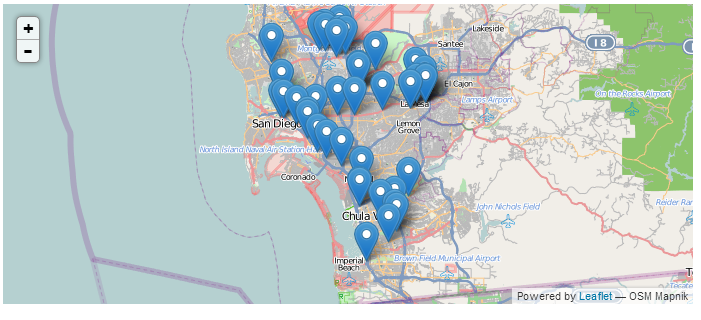
\includegraphics[width=.8\textwidth]{fig/leaflet-osmmapnik}
  \caption{Leaflet with OSM mapnik tile layer}
  \captionsetup{font={footnotesize,bf,it}}
  \caption*{source: \url{http://drupal.org/}}
  \label{fig:leaflet1}
\end{figure} 

\begin{description}
\item[tiles:] Tiles are square bitmap graphics displayed on a grid fashion in order to show a map. Tile layers are defined by a URL from which the images will be obtained and the library will take care of displaying the appropriate grid depending on the zoom level and the view box. The tiles used change drastically the looks of the map, an example of the OSM mapnik tiles can be found in figure \ref{fig:leaflet1}.

\item[vectors:] These layers are used to display information about features on the map in form of geometries. Vector layers can be classified into five categories, three of them corresponding to the typical vector representation on GIS systems: lines, polygons, points, rectangles and circles. Layers can be added and removed from the map easily as shown in example \ref{lst:leaflet2}

\item[layer groups:] The last kind of layers are simply used as a convenience to manipulate more than one feature at the same time. One kind of layer group is the GeoJSON layer which allows the creation of layers from GeoJSON files, detailed in section \ref{sec:geojson}.

\end{description}

\begin{listing}[ht]\centering
  \begin{minipage}{.7\textwidth}
    \begin{minted}[linenos=true,mathescape,gobble=6]{javascript}
	     var bounds = [[54.559322, -5.767822], [56.1210604, -3.021240]];
	     L.rectangle(bounds, {color: "#ff7800", weight: 1}).addTo(map);
	     var point = L.marker([50.5, 30.5]);
	     //A popup can be bound to be shown on click
	     point.bindPopup("This is a popup message");
    \end{minted}
  \end{minipage}
  \caption{Leaflet layers.}\label{lst:leaflet2}
\end{listing}

\subsection*{Interaction}

Leaflet is built with the idea of creating interactive maps, thus, it offers methods for manipulating the map and firing and receiving events. It is possible to register listener on map actions, such as when a map is moved or zoomed, or to register listeners on layers, to check when a layer is added, removed, clicked, etc.

This way, it is possible to respond to user actions via callbacks. The framework provides some shortcuts, for example, it is possible to bind the showing of a small popup to the click on a marker without the need to register a callback, as shown in listing \ref{lst:leaflet2}

Another example on the usage of leaflet events can be found in listing \ref{lst:leaflet3}. In the example, a callback is registered for the event of the user moving the map. This is useful for updating the map with information from the layers on the current view.

\begin{listing}[ht]\centering
  \begin{minipage}{.5\textwidth}
    \begin{minted}[linenos=true,mathescape,gobble=6]{javascript}
	     // The moveend event is fired every time the
	     // map is moved, dragged or zoomed
	     Map.map.on('moveend', function(){
	       //Obtain the current bounding box of the map
	       var bbox = Map.map.getBounds().toBBoxString();
	       var feature = queryTheServer(bbox);
	       map.addLayer(features);
	     });
    \end{minted}
  \end{minipage}
  \caption{Leaflet layers.}\label{lst:leaflet3}
\end{listing}

\subsection*{Why Leaflet?}

There are not many alternatives when it comes to create JavaScript based maps. Google maps can be used to embed a map on a web page, however, it does not offer much interaction and can hardly be used for other than displaying static data. OpenLayers is another alternative, however, it is known to be hard to learn and the community using it is smaller that Leaflet's one. The amount of developers using leaflet provides the framework with a good deal of extensions and its ease of use make it easy to work with even for novice developers.

\section{Phonegap}\label{sec:phonegap}

Desktop computers are not the only devices that have seen a rise in computational power in the last years, smartphones and other mobile devices have also improved significantly. 

Interaction, screens and even browser support are drastically different in desktop and mobile; and the latter still suffers from a lack of computational power. Due to this web development is not so easily applicable to these devices, building a mobile friendly web application is a difficult task.

However, due to the shift from native to web development happening on desktops, most developers have already learned the tools for developing HTML5 applications. This together with the popularity of mobile apps and difficulty of developing multi-platform applications, has given rise to a number of tools designed to code native mobile applications using HTML5, CSS3 and JavaScript.

The leading among these is Phonegap. Phonegap is a framework that allows to create mobile apps using standardized web APIs for all the major platforms \cite{phonegap}. 

\subsection*{HTML5 development}

The development tools used on a Phonegap application are identical to those used on a regular web page. HTML documents are used to structure the views, CSS stylesheets are used to define the appearance of the application and JavaScript is used to program the behavior.

This is possible because what the library does is opening a enhanced web view (a browser) on the mobile device and loading the files into it. Normally, this would mean that much of the sensors of the device, such as the camera and the gyroscope are not usable, however, the browser created by the framework is extended to allow access to all the hardware on the device.

Phonegap is based on Apache Cordova \cite{apachecordova} which works with a set of plugins. These plugins provide the web view with the functionality it lacks, and expose it as JavaScript APIs. One example of this is the reading of the battery status, as shown on listing \ref{lst:phonegap1}. Aside from the plugins that come shipped with the core libraries, the community has developed a considerable amount of them to provide functionalities that mobile browsers usually lack, such as HTML5 web socket support.

\begin{listing}[ht]\centering
  \begin{minipage}{.8\textwidth}
    \begin{minted}[linenos=true,mathescape,gobble=6]{javascript}
	     window.addEventListener("batterystatus", onBatteryStatus, false);
	     
	     function onBatteryStatus(info) {
	         console.log("Level: " + info.level + " isPlugged: " + info.isPlugged);
	     }
    \end{minted}
  \end{minipage}
  \caption{Reading battery status with Phonegap.}\label{lst:phonegap1}
\end{listing}

\subsection*{Phonegap Build}

As convenient using HTML5 for developing cross platform applications is, there is still a need to configure the build for each of the platforms and to install the corresponding Software Development Kits (SDKs) which can be tedious and time consuming.

In the face of this issue, Phonegap offers a platform called Phonegap Build, a cloud based service which helps agile development and allows to compile applications for six of the seven platforms supported by the framework. The Phonegap team illustrated this process in figure \ref{fig:phonegapbuild} on their web page.

\begin{figure}[h]
  \centering
  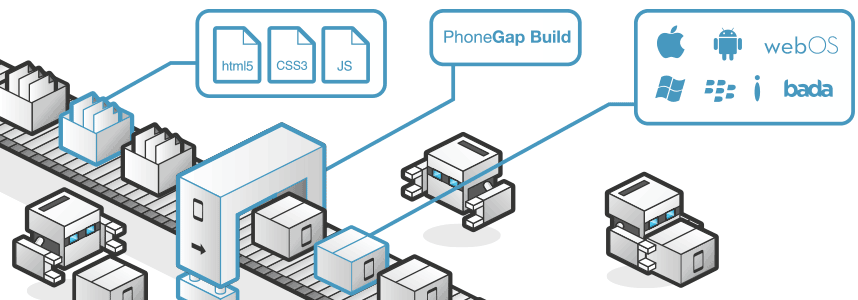
\includegraphics[width=.8\textwidth]{fig/phonegap-build}
  \caption{Phonegap Build process}
  \captionsetup{font={footnotesize,bf,it}}
  \caption*{source: \url{http://phonegap.com/about/}}
  \label{fig:phonegapbuild}
\end{figure} 

\subsection*{Why Phonegap?}

In the world of mobile HTML5 development there are not many competitors. Phonegap is the leading platform, followed by Appcelerator and Ionic. Still, Phonegap is the most mature of them all and has the biggest community, which results in a higher amount of plugins offering more functionality.

On the other side, native development is out of consideration. One of the requirements of the project is for the mobile application to be multi-platform and while developing it natively may increase performance, the payback in development times would be too much. Besides, since the mobile application interfaces and interaction are heavily map based, the code used on other parts of the project can be reused.

Thus, the decision to use Phonegap is made, based on the cut on development times, the re usability of code and the fact that there is no need to learn other development languages.

\section{GPX}\label{sec:gpx}

GPX is a lightweight XML data format for the interchange of GPS data (tracks, routes and way points) between applications and web services on the Internet \cite{gpx}. GPX was released in 2004 and has since then been the de facto standard when it comes to the encoding and interchange of GPS data.

The format represents three types of data, in the following manner:

\begin{description}
\item[Way points:] A way point is a set of coordinates that identifies a point in space. They are represented using the \texttt{<wpt>} tag, as shown in listing \ref{lst:gpx1}

\begin{listing}[ht]\centering
  \begin{minipage}{.5\textwidth}
    \begin{minted}[linenos=true,mathescape,gobble=6]{xml}
	     <wpt lat="42.438878" lon="-71.119277">
	       <ele>44.586548</ele>
	       <time>2001-11-28T21:05:28Z</time>
	       <name>Example waypoint</name>
	     </wpt>
    \end{minted}
  \end{minipage}
  \caption{GPX way point representation.}\label{lst:gpx1}
\end{listing}


\item[Tracks:] A track is a segment containing way points, that is, a set of coordinates that describe a path. In GPX tracks are represented by the \texttt{trk} element and point inside one by \texttt{trkpt} elements (see listing \ref{lst:gpx2}).

\begin{listing}[ht]\centering
  \begin{minipage}{.5\textwidth}
    \begin{minted}[linenos=true,mathescape,gobble=6]{xml}
	     <trk>
	       <name>Example GPX Document</name>
	       <trkseg>
	         <trkpt lat="47.644548" lon="-122.326897">
	           <ele>4.46</ele>
	           <time>2009-10-17T18:37:26Z</time>
	         </trkpt>
	       </trkseg>
	      </trk>
    \end{minted}
  \end{minipage}
  \caption{GPX track representation.}\label{lst:gpx2}
\end{listing}

\item[Routes:] A route is identical to a track in its encoding, with the difference that the tags \texttt{rte} and \texttt{rtept} are used (see listing \ref{lst:gpx3}). However, there is a difference in the meaning of this concepts; while a track is a record of where a person has been, a route is a suggestion about where someone might go in the future. For this reasons, tracks may have timestamps attached while routes will not.

\begin{listing}[ht]\centering
  \begin{minipage}{.5\textwidth}
    \begin{minted}[linenos=true,mathescape,gobble=6]{xml}
	     <rte>
	       <name> Example route </name>
	       <rtept lat="47.644548" lon="-122.326897">
	         <name>Example route point</name>
	       </rtept>
	     </rte>
    \end{minted}
  \end{minipage}
  \caption{GPX route representation.}\label{lst:gpx3}
\end{listing}

\end{description}

\subsection*{Why GPX?}

GPX has been the de facto standard when it comes to representing and interchanging trail and points of interest on the web for ten years. Because of this, it is unreasonable to think in a system which allows interchange of GPS data without using this format. Together with the completeness of the information provided by a GPX file, these are two solid reasons for the usage of GPX on the platform.

\section{GeoJSON}\label{sec:geojson}

GeoJSON is a format for encoding a variety of geographic data structures \cite{geojson}. GeoJSON objects may represent a geometry, a feature or a collection of features (see section \ref{sec:geosparql}, GeoSPARQL). The following geometry types are supported: 
\begin{itemize}
\item \texttt{Point}
\item \texttt{LineString}
\item \texttt{Polygon}
\item \texttt{MultiPoint}
\item \texttt{MultiLineString}
\item \texttt{MultiPolygon} 
\item \texttt{GeometryCollection}.
\end{itemize}

More than a file format in itself, it is a specification of how to encode geographical features in JSON format. A complete GeoJSON data structure is always a JSON object, which consists in a collection of key-value pairs, being the key a string and the values any other kind of data.

The specification defines GeoJSON objects in the following way:

\begin{itemize}
\item A GeoJSON object may have any number of members (name/value pairs).
\item The GeoJSON object may have a member with the name \texttt{type}. Its value will be a string that determines the type of the object.
\item The value of the type member must be one of: \texttt{Point}, \texttt{MultiPoint}, \texttt{Polygon}, \texttt{MultiPolygon}, \texttt{LineString}, \texttt{MultiLineString}, \texttt{GeometryCollection}, \texttt{Feature} or \texttt{FeatureCollection}.
\item A GeoJSON object may have an optional member of name \texttt{crs} which specifies the coordinate reference system.
\item A GeoJSON object may have a \texttt{bbox} member, whose value must be a bounding box array.
\end{itemize}

\subsection*{Geometries}

Geometries are GeoJSON objects whose type is different from \texttt{Feature} or \texttt{FeatureCollection}. These elements, unless they are of type \texttt{GeometryCollection}, must have a member of name \texttt{coordinates} which specifies the coordinates of the object in an array of positions.

Positions are represented by an array of numbers, one for the longitude, one for the latitude and an optional one for the elevation, in that order. The coordinates of a object are formed by a array of positions, except for \texttt{Point} element, which have a single position.

A \texttt{GeometryCollection} must have a member named \texttt{geometries}, an array of GeoJSON geometry objects. An example of this can be found on listing \ref{lst:geojson1}.

\begin{listing}[ht]\centering
  \begin{minipage}{.6\textwidth}
    \begin{minted}[linenos=true,mathescape,gobble=6]{json}
	      { "type": "GeometryCollection",
	         "geometries": [
	           { "type": "Point",
	             "coordinates": [100.0, 0.0]
	             },
	           { "type": "LineString",
	             "coordinates": [ [101.0, 0.0], [102.0, 1.0] ]
	             }
	         ]
	       }
    \end{minted}
  \end{minipage}
  \caption{A GeoJSON \texttt{GeometryCollection} object.}\label{lst:geojson1}
\end{listing}

\subsection*{Features}

A Feature is a object with some spatial representation. A feature must have two essential members, aside from the type, which are \texttt{geometry} and \texttt{properties}. The first of these members must contain a GeoJSON geometry object, the spatial representation of the object.

The \texttt{properties} member on the other side, is a regular JSON object (a name/value dictionary) and contains all the non-spatial data belonging to the feature. A \texttt{FeatureCollection} does not contain a \texttt{geometry} member, instead it has a \texttt{features} object, an array of feature object in the collection. An example of a feature is shown on listing \ref{lst:geojson2}

\begin{listing}[ht]\centering
  \begin{minipage}{.8\textwidth}
    \begin{minted}[linenos=true,mathescape,gobble=6]{json}
	        { "type": "Feature",
	          "bbox": [-180.0, -90.0, 180.0, 90.0],
	          "geometry": {
	            "type": "Polygon",
	            "coordinates": [[
	              [-180.0, 10.0], [20.0, 90.0], [180.0, -5.0], [-30.0, -90.0]
	              ]]
	            },
	            "properties": {
	              "name": "Example feature"
	            }
	          }
    \end{minted}
  \end{minipage}
  \caption{A GeoJSON \texttt{Feature} object.}\label{lst:geojson2}
\end{listing}





\chapter{Requirements Specification}\label{ch:requirements}

\section{Overview}

This chapter provides a specifications of the requirements, both functional and non-functional, that the project to be developed must satisfy, which define the overall functioning of the system to be produced. Each requirement will have a code associated for identification purposes.

To achieve a better understanding of these requirements, they are divided into the following sections, each corresponding to a different phase of product of the project.

\begin{itemize}
\item \textbf{Requirements of the ontology:} The requirements to be satisfied by the ontology as well as a minimum subset of classes and properties it must have are listed.
\item \textbf{Requirements of the server:} The requirements to be satisfied by the server and the system overall are defined in this section.
\item \textbf{Requirements of the web application:} The requirements to be satisfied by the web client are defined in this section.
\item \textbf{Requirements of the mobile application:} The requirements to be met by the mobile client are defined in this section.
\item \textbf{Non-functional requirements:} The requirements which don't specify any particular .
\end{itemize}

\section{Requirements for the ontology}

The requirement for the ontology are the ones which define the characteristics that the vocabulary to be produced must meet. This requirements are listed below:

\begin{description}
\item[RONT1] The ontology must support spatial reasoning.
\item[RONT2] The ontology must support the following inference mechanisms:
\begin{itemize}
\item disjoint classes
\item subclasses
\item subproperties
\item inverse properties
\item symmetric properties
\item functional properties
\item maximum cardinalities
\end{itemize}
\item[RONT3] The ontology must be designed following Linked Open Data best practices, so it should reuse existing vocabularies.
\item[RONT4] The ontology must represent the following types of resources:
\begin{itemize}
 \item Features
 \begin{itemize}
  \item Trails
  \item Points of Interest
  \item Geolocated Notes
 \end{itemize}
 \item Persons
 \item Multimedia Resources
 \begin{itemize}
  \item Text
  \item Images
  \item Video
 \end{itemize}
\end{itemize}
\item[RONT5] The resources of type \textit{Trail} must contain the information below:
\begin{itemize}
\item name
\item description
\item difficulty score
\item maximum altitude
\item minimum altitude
\item ascending slope
\item descending slope
\item posts
\item images
\item author
\item persons who traversed it
\item coordinates
\end{itemize}
\item[RONT6] The resources of type \textit{Point of Interest} must contain the following information:
\begin{itemize}
\item name
\item description
\item altitude
\item category
\item posts
\item images
\item author
\item coordinates
\end{itemize}
\item[RONT7] The resources of type \textit{Geolocated Note} must contain the following information:
\begin{itemize}
\item text
\item multimedia
\item author
\item privacy level
\item creation time
\item duration
\item action radius
\item coordinates
\end{itemize}
\item[RONT8] Resources of type \textit{Person} must contain the following information:
\begin{itemize}
\item nickname
\item email
\item first name
\item family name
\item avatar
\item description
\item people in which is interested
\item trail buddies
\item optionally external homepage
\item added trails
\item added points of interest
\item added notes
\item added multimedia
\end{itemize}
\item[RONT9] Multimedia resources of type \textit{Text} must contain the following information.
\begin{itemize}
\item author
\item content
\item feature they belong to
\end{itemize}
\item[RONT10] Multimedia resources of type \textit{Image} and \textit{Video} must contain the following information.
\begin{itemize}
\item author
\item download link
\item addition date
\item feature they belong to
\end{itemize}
\end{description}

\section{Requirements specification for the server}

The requirements for the server specify the functionality that the server must implement as well as the function and resources exposed by the API and overall inter-component communication, for the server is the central piece of the system.

\begin{description}
\item[RSV1] The system must be able to operate on Points.
\item[RSV2] The system must be able to operate on LineStrings.
\item[RSV3] The server must be able to obtain the following data from a LineString representing a trail.
 \begin{itemize}
 \item distance
 \item difficulty
 \item ascending slope
 \item descending slope
 \item maximum altitude
 \item minimum altitude
 \end{itemize}
\item[RSV4] The system must be able to create and send SPARQL queries to a data store.
\item[RSV5] The system must be able to retrieve data from Geonames and OpenStreetMap and aggregate it to the dataset.
\item[RSV6] The server must expose a SPARQL read-only endpoint.
\item[RSV7] The server must expose a public API.
\item[RSV8] The public API must follow the REST style.
\item[RSV9] The API must expose the following resources
  \begin{itemize}
  \item Trails
  \item Points of Interest
  \item Geolocated Notes
  \item Users
  \end{itemize}
\item[RSV10] The resources must expose the following operations:
  \begin{itemize}
  \item Read
  \item Update (Except Geolocated Notes)
  \item Create
  \end{itemize}
\item[RSV11] The resources must expose information about other related resources, such as posts, images, etc.
\item[RSV12] The API must offer additional operations which expose the following functionality:
  \begin{itemize}
  \item Search
  \item Features within a area
  \item Features near each other
  \item Information about the system
  \item Information about the API
  \end{itemize} 
\item[RSV13] The server must offer secure authentication.
\item[RSV14] The system must be able to provide recommendations based on preferences and location.
\item[RSV15] The system must be able to store user preferences, for recommendation and filtering purposes.
\item[RSV16] Signing in the system will be done via e-mail and password.
\end{description}

\section{Requirements of the web application}

The requirements for the web application detail the constraints that the web based client must fulfill, as well as the functionality that need to be implemented.

\begin{description}
\item[RWEB1] The web application must work on most major browsers. The minimum browsers specified are the following:
  \begin{itemize}
  \item Google Chrome 26
  \item Mozilla Firefox 22
  \item Safari 6
  \item Internet Explorer 10
  \item Opera 12
  \end{itemize}
\item[RWEB2] The web application must communicate with the server using the public API.
\item[RWEB3] The web application will have a homepage presenting the platform and linking to the rest of the sections.
\item[RWEB4] The web application must have a section allowing the following features:
  \begin{itemize}
  \item Explore data based on its location
  \item Draw and edit trails and points of interest
  \end{itemize}
\item[RWEB5] The web application must have a section which provides the following functionality.
  \begin{itemize}
  \item Search over the data on the system
  \item Upload a trail or point of interest from a GPX file
  \item View detailed information about any data on the platform
  \end{itemize}
\item[RWEB6] The web application must have a section which provides the following features:
  \begin{itemize}
  \item Register a user on the system
  \item Log in the system
  \item Modify the profile of a user
  \end{itemize}
\item[RWEB7] All geographic data must be shown on a interactive map.
\item[RWEB8] All operations that require manipulation of spatial data have to be performed without any need of GIS knowledge from the user.
\item[RWEB9] Signing in only has to be needed for write operations.
\item[RWEB10] Registering a user via web platform will require the following information:
  \begin{itemize}
  \item User name
  \item Email
  \item Password
  \end{itemize}
\item[RWEB11] Creating a trail via web platform will require the following information:
  \begin{itemize}
  \item Name
  \item Description
  \item Geographic representation
  \end{itemize}
\item[RWEB12] Creating a point of interest via web platform will require the following information:
  \begin{itemize}
  \item Name
  \item Description
  \item Category
  \item Geographic representation
  \end{itemize}
    
\end{description}

\section{Requirements of the mobile application}

The requirements to the mobile specify the operations that can be done with the mobile application and the functionality it must implement.

\begin{description}
\item[RMOB1] The application must allow the recording of a trail.
\item[RMOB2] The application must allow exporting trails in GPX format or uploading them to the system when a network connection is available.
\item[RMOB3] The application must allow the creation of Geolocated Notes on the current position of the user.
\item[RMOB4] The application must keep track of the current position of the user at all times.
\item[RMOB5] The application must be able to receive real time notifications of nearby features.
\item[RMOB6] The application must be able to notify the user when a new feature is discovered, even if it is not currently active.
\item[RMOB7] The application must allow search and detailed view of information on the system.
\item[RMOB8] The application must provide log in and registration functionalities.
\item[RMOB9] The application can only be used by registered users.
\item[RMOB10] Registering a user via mobile platform will require the following information:
  \begin{itemize}
  \item User name
  \item Email
  \item Password
  \end{itemize}
\item[RMOB11] Creating a trail via mobile platform will require the following information:
  \begin{itemize}
  \item Name
  \item Description
  \item Recording of the trail
  \end{itemize}
\item[RMOB11] Creating a geolocated note via web mobile platform will require the following information:
  \begin{itemize}
  \item Text, Image or video
  \item Privacy level
  \item Range
  \item Coordinates
  \end{itemize} 
\item[RMOB12] Once signed in the mobile application, the system will store the password and username, for convenience purposes.
\end{description}

\section{Non-functional requirements}

The requirements not belonging to a specific category are listed in this sections. This refers to information visibility and privacy, performance and user interaction issues mainly.

\begin{description}
\item[RNF1] All the information, except a few sensible data, has to be published according to Linked Open Data best practices.
\item[RNF2] The following data must be kept private:
  \begin{itemize}
  \item User passwords
  \item The current location of the users
  \end{itemize}
\item[RNF3] The server should be able to handle high loads of connection.
\item[RNF4] The interface on the web application must be responsive, that is, the interface must adapt to mobile and tablet devices.
\item[RNF5] The web application must have a fast loading time and small memory footprint, in order to be adapted to mobile devices.
\item[RNF6] The applications must have intuitive and easy to use and read interfaces.
\item[RNF7] The style of the mobile and web applications must be similar.
\end{description}
\chapter{Design specification}\label{ch:design}

\section{Overview}

This section describes the design work done through the project as well as the tools used to carry that labor and the results of it. The chapter covers the following topics:

\begin{itemize}
\item \textbf{Architecture of the system:} The chosen architecture of the system is described, together with the reasons and advantages of the design.
\item \textbf{Design of the ontology:} The final design of the ontology is described, as well as it's advantages in front of other data modeling paradigms.
\item \textbf{Design of the central server:} The class design of the server is detailed in this section.
\item \textbf{Design of the web application:} The class design of the web application is detailed in this section, as well as the interface design.
\item \textbf{Design of the mobile application:} The class design of the mobile application is detailed in this section, as well as the interface design.
\item \textbf{Development environment:} The list of technologies employed in the project is detailed, briefly explaining the role of each tool.

\end{itemize}

\section{System architecture}\label{sec:designarch}

Figure \ref{fig:architecture} shows the architecture chosen for the system. This architecture comprises the following elements:

\begin{itemize}
\item A central server
  \begin{itemize}
  \item Web server
  \item SPARQL endpoint
  \item REST API
  \item Data agregator
  \item Database connector
  \end{itemize}
\item A semantic spatial storage system which contains the ontology
\item A web client used as the main interface of the system
\item A mobile application to support the browser based one
\end{itemize}

\begin{figure}[ht]
  \centering
  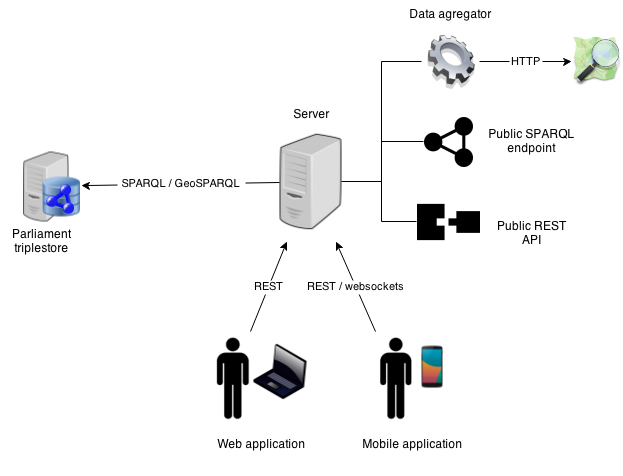
\includegraphics[width=.8\textwidth]{fig/architecture}
  \caption{Architecture design of the system}
  \captionsetup{font={footnotesize,bf,it}}
  \label{fig:architecture}
\end{figure} 

\subsection{Central server}

The central server is the core component of the system. It implements most of the functionality on the system and provides data to the client. It also analyzes the trails uploaded to the system and takes care of the communication with the database. The server is divided into several logical software pieces, which are described below.

\subsubsection*{Database connector}

The database connector implements the functionality needed to connect with the semantic data store. In essence, this means that it takes the requests from the users and transforms them into SPARQL queries. Then it takes the results provided by the database and converts them into a format that the server can process.

\subsubsection*{The data agregator}

This component has the function of querying external data sources and adapting the results to the data model of the system. It is independent of the rest of components of the server, since instead of being available to receive requests it will just run on demand. The component makes HTTP queries to the different APIs and endpoints on the web, for example OpenStreetMap and Geonames, and aggregates the data to the database.

\subsubsection*{REST API}

The API provides the basic means of accessing the information on the system. It is used by both clients to communicate with the server. It can be used for read, write and update operations, however, delete operations are not contemplated.

\subsubsection*{The SPARQL endpoint}

This endpoint just routes SPARQL queries done to it to the database. Its role is related to filtering the queries that seek to write and to ensure that no petition is going to break the integrity of the data in the database.

\subsection{Semantic spatial storage system}

This component of the system is mostly third party software. It consists on a triple store, a data storage system that stores RDF data; a reasoner supporting OWL and GeoSPARQL and an HTTP SPARQL endpoint. This component also englobes the ontology designed to define the data model of the system. This ontology is described in detail in section \ref{sec:ontdesign}.

\subsection{Web client}

The web client is the main interface though which the system is accessed. It communicates with the server through a REST API and offers most of the functionality of the system to the users.

The client may be used from desktop browsers or mobile browser with no restrictions. More details on the design of the client can be found on section \ref{sec:webappdesign}.

\subsection{Mobile application}

The mobile client provides the functionality that the web application cannot. It provides real time functions by using a websocket API that the server exposes. The design of this component is detailed in section \ref{sec:mobileappdesign}.

\section{Design of the ontology}\label{sec:ontdesign}

The ontology designed in the project represents specific knowledge related to the domain of Trails, Points of Interest and GPS data in general. It uses external ontologies as a base, in order to ease the sharing of information and the publishing of the dataset at Linked Open Data.

\begin{figure}[ht]
  \centering
  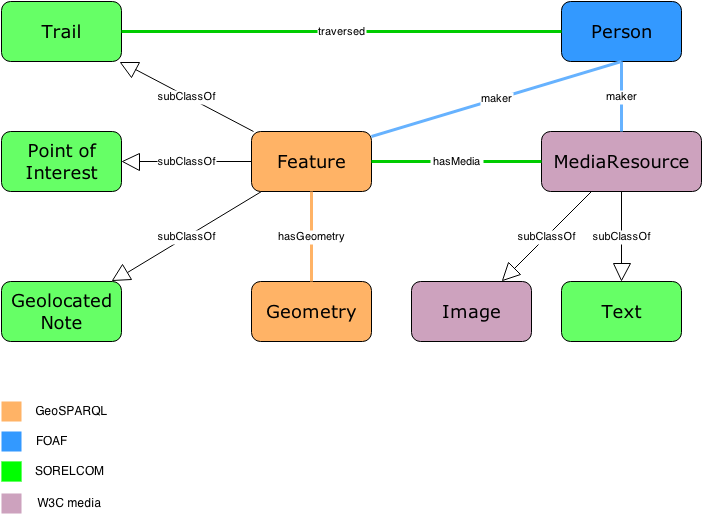
\includegraphics[width=.8\textwidth]{fig/sorelcom-ontology}
  \caption{The SORELCOM ontology}
  \captionsetup{font={footnotesize,bf,it}}
  \label{fig:sorelcom-ontology}
\end{figure} 

Figure \ref{fig:sorelcom-ontology} provides a graphical representation of classes on the SORELCOM ontology. As shown on the figure, classes from three vocabularies are reused. The FOAF vocabulary is used to obtain a representation of the users of the platform, the GeoSPARQL vocabulary is used as a base for all the resources with a spatial character and the W3C media vocabulary is used to represent the media resources on the platform.

The focus of the design is to reuse as many well known vocabularies as possible and defining the needed classes, relations and properties to satisfy the requirements of the ontology 4 to 10, defined in chapter \ref{ch:requirements}.

\subsection{Class hierarchy}

The ontology defines a series of classes for the representation of specific spatial features present in the domain of the application. The classes are listed below:

\begin{description}
\item[\texttt{sorelcom:Trail}] A trail represents a path in the world. In the context of the application, a trail can be interpreted as a path that a user has traversed or as a simple route that is indicated by a user, however, the ontology does not specify that a trail should have any of these meanings.

\item[\texttt{sorelcom:PointOfInterest}] A Point of Interest is a feature in the world that may result of some interest for a person. There is no specification on what can be the interest a person may have on the feature, thus a point of interest may be anything from a monument to a restaurant.

\item[\texttt{sorelcom:GeolocatedNote}] A Geolocated Note is a message with a spatial context. This message is left by a person at a specific location, and can be viewed by any person or just a specific group depending on its privacy settings. The message on a note may be formed by text, images, video or any combination of them.
\end{description} 

In addition to the core types on the vocabulary, other classes obtained from external ontologies will be used or extended to represent different types of resources on the ontology. The additional classes used are the following:

\begin{description}
\item[\texttt{foaf:Person}] This class is used to classify resources as persons. Any user on the system will be classified as person. The class is defined in the FOAF vocabulary.

\item[\texttt{geo:Feature}] A feature is any object in the real world that has a spatial representation. \textit{Trails}, \textit{Points of Interest} and \textit{Geolocated Notes} are all types of Features. This class is defined in the GeoSPARQL vocabulary.

\item[\texttt{geo:Geometry}] In the GeoSPARQL ontology, a geometry is used to give a spatial representation to a Feature. Without a associated feature, geometries are not resources on the real world.

\item[\texttt{media:MediaResource}] A media resource is a representation of a media object, such as a image or a video. Media resources refer to the images, posts and videos saved in the system.

\item[\texttt{media:Image}] A image is a specialized media resource, which refers to a image. It is used in conjunction with the \texttt{sorelcom:Text} class to represent the specific type of a media in the system.
 
\end{description}

\subsection{Properties}

Most of the work on the design of the ontology consists on the creation of properties which relate the resources to the information that they must contain. Still, many of the properties used in the data model of the platform are obtained from external vocabularies.

The properties defined for the SORELCOM vocabulary are listed below, together with a table representing how the information about those resources is stored in the data model:

\subsubsection*{Feature properties}

\begin{description}
\item[\texttt{sorelcom:name}] Property representing the human readable name of a feature. 
\item[\texttt{sorelcom:description}] Property representing a textual description of a feature.
\item[\texttt{sorelcom:hasMedia}] Property relating a feature to the media associated. It is the inverse of \texttt{sorelcom:mediaOf}.
\end{description}

\subsubsection*{Trail properties}

\begin{description}
\item[\texttt{sorelcom:difficulty}] Property representing the difficulty score of a trail. This score is a integer from 0 to 100, the higher the difficulty the higher the number. A trail may only have one difficulty.
\item[\texttt{sorelcom:maximumAltitude}] Property representing the altitude of the highest point of a trail.
\item[\texttt{sorelcom:minimumAltitude}] Property representing the altitude of the lowest point of a trail.
\item[\texttt{sorelcom:totalDistance}] Property representing the total distance in meters that must be traversed from the starting point of a trail to the end of it.
\item[\texttt{sorelcom:ascendingDistance}] Property representing the sum of the distance in meters of the segments of the trail which are ascendant .
\item[\texttt{sorelcom:descendingDistance}] Property representing the sum of the distance in meters of the segments of the trail which are descendant.
\item[\texttt{sorelcom:circular}] Property representing if the starting point and end point of a trail are the same.
\item[\texttt{traversedBy}] Property relating a trail to the users who have traversed it.
\end{description}

Information about how trails are represented on the system can be found on table \ref{tab:trail}.

\begin{table}[ht]
  \centering
  \caption{Trails on the SORELCOM data model.}\label{tab:trail}
  \begin{tabular}{llll}
    \toprule
      \textbf{Property} & \emph{domain}  & \emph{range} & \emph{information}\\
    \midrule
      sorelcom:name & geo:Feature  & string & name \\
      sorelcom:description & geo:Feature & string  & description \\
      sorelcom:difficulty & sorelcom:Trail & integer & difficulty \\
      sorelcom:maximumAltitude & sorelcom:Trail & float & maximum altitude \\
      sorelcom:minimumAltitude & sorelcom:Trail & float & minimum altitude \\
      sorelcom:ascendingDistance & sorelcom:Trail & integer & ascending distance \\
      sorelcom:descendingDistance & sorelcom:Trail & integer & descending distance \\
      sorelcom:hasMedia & geo:Feature & ma:Media & images, posts \\
      foaf:maker & Thing & foaf:Person & author \\
      sorelcom:traversedBy & sorelcom:Trail & foaf:Person & persons who traversed it \\ 
      geo:hasGeometry & geo:Feature & geo:Geometry & spatial representation \\
    \bottomrule
  \end{tabular}
\end{table}

\subsubsection*{Point of interest properties}

\begin{description}
\item[\texttt{sorelcom:altitude}] Property representing altitude of the point. 
\item[\texttt{sorelcom:category}] Property representing the category of the point of interest.
\end{description}

Information about how points of interest are represented on the system can be found on table \ref{tab:poi}.

\begin{table}[ht]
  \centering
  \caption{Points of interest on the SORELCOM data model.}\label{tab:poi}
  \begin{tabular}{llll}
    \toprule
      \textbf{Property} & \emph{domain}  & \emph{range} & \emph{information}\\
    \midrule
      sorelcom:name & geo:Feature  & string & name \\
      sorelcom:description & geo:Feature & string  & description \\
      sorelcom:altitude & sorelcom:PointOfInterest & float & altitude \\
      sorelcom:category & sorelcom:PointOfInterest & string & category \\
      sorelcom:hasMedia & geo:Feature & ma:Media & images, posts \\
      foaf:maker & Thing & foaf:Person & author \\
      geo:hasGeometry & geo:Feature & geo:Geometry & spatial representation \\
    \bottomrule
  \end{tabular}
\end{table}

\subsubsection*{Geolocated Note properties}

\begin{description}
\item[\texttt{sorelcom:range}] Property representing range of action of a Geolocated Note. 
\item[\texttt{sorelcom:public}] Property representing if the note is public.
\item[\texttt{sorelcom:targets}] Property relating the note to the persons that should receive it. It exists only when the note is not public.
\end{description}

Information about how geolocated notes are represented on the system can be found on table \ref{tab:note}.

\begin{table}[ht]
  \centering
  \caption{Geolocated notes on the SORELCOM data model.}\label{tab:note}
  \begin{tabular}{llll}
    \toprule
      \textbf{Property} & \emph{domain}  & \emph{range} & \emph{information}\\
    \midrule
      dcterms:created & Thing & date & creation time \\
      dcterms:valid & Thing & date or integer & duration \\
      sorelcom:public & sorelcom:GeolocatedNote & boolean & privacy level \\
      sorelcom:radius & sorelcom:GeolocatedNote & integer & action radius \\
      sorelcom:hasMedia & geo:Feature & ma:Media & text, multimedia \\
      foaf:maker & Thing & foaf:Person & author \\
      geo:hasGeometry & geo:Feature & geo:Geometry & spatial representation \\
    \bottomrule
  \end{tabular}
\end{table}

\subsubsection*{Person properties}

\begin{description}
\item[\texttt{sorelcom:hasTraversed}] Property relating a Person to the trails it has traversed.
\item[\texttt{sorelcom:trailBuddyOf}] Property relating a Person to his/her trail buddies, that is, people who are usual sports or tourism mates.
\end{description}

Information about how persons are represented on the system can be found on table \ref{tab:user}.

\begin{table}[ht]
  \centering
  \caption{Persons on the SORELCOM data model.}\label{tab:user}
  \begin{tabular}{llll}
    \toprule
      \textbf{Property} & \emph{domain}  & \emph{range} & \emph{information}\\
    \midrule
      foaf:nick & foaf:Person  & string & nickname \\
      foaf:mbox & foaf:Person  & string & email \\
      foaf:firstName & foaf:Person  & string & first name \\
      foaf:familyName & foaf:Person  & string & family name \\
      foaf:depiction & foaf:Person  & foaf:Image & avatar \\
      sorelcom:trailBuddyOf & foaf:Person  & foaf:Person & trail buddies \\
      sorelcom:hasTraversed & foaf:Person & sorelcom:Trail & traversed trails \\
      foaf:weblog & foaf:Person  & URI & external homepage \\
      foaf:made & foaf:Person  & Thing & features and media \\
    \bottomrule
  \end{tabular}
\end{table}

\subsubsection*{Media properties}

\begin{description}
\item[\texttt{sorelcom:mediaOf}] Property relating a media resource to the feature it belongs to.
\end{description}

Information about how media resources are represented on the system can be found on table \ref{tab:media}. Media resources are divided into images, text and video, however, for convenience purposes all of them are presented in a single table. The only properties that are not shared among all media resource types are the content and the download link. The content is only used in the text, while the download link is used on media images and video.

\begin{table}[ht]
  \centering
  \caption{Media on the SORELCOM data model.}\label{tab:media}
  \begin{tabular}{llll}
    \toprule
      \textbf{Property} & \emph{domain}  & \emph{range} & \emph{information}\\
    \midrule
      foaf:maker & Thing & foaf:Person & author \\
      ma:description & ma:MediaResource & string & content \\
      ma:locator & ma:MediaResource & URI & download link \\
      dcterms:created & Thing & datetime & addition date \\
      sorelcom:mediaOf & ma:MediaResource & geo:Feature & feature \\
    \bottomrule
  \end{tabular}
\end{table}

\subsection*{Inference mechanism}

In order to get the maximum benefit from the semantic dataset the ontology has been defined using OWL. Due to this, several inference mechanism have been available during the design process, however, only a subset of them have been used. The following inference mechanisms have been used:

\begin{description}
\item[Sub classes] All resources which are instanced of a certain class A are also instances of the classes A is subclass of. This property is provided by RDF schema (see section \ref{sec:rdf} for more information). In RDF it is possible to use multiple inheritance, meaning that a class can be subclass of more than one class.
\item[Disjoint classes] A group of disjoint classes indicate that a resource of one class of the group cannot be of another class on the group
\item[Sub properties] Subproperty relations are the analogous of subclass relations when referring to resources of type property. It is also provided by RDF schema.
\item[Function properties] A functional property is a property that can only appear once in the triples of a certain resource. It is provided by OWL lite.
\item[Inverse properties] When a resource A is related to B by a property P1, then B is related to A by the property P2 inverse of P1. It is provided by OWL lite.
\item[Symmetric property] When a resource A is related to B by a symmetric property P, then B is related to A also by P.

\end{description}

Table \ref{tab:inferencecls} shows the inference rules used on the classes of the ontology and \ref{tab:inferenceprop} shows the inference rules used on the properties of the data model.

\begin{table}[ht]
  \centering
  \caption{Inferences used on the SORELCOM ontology classes.}\label{tab:inferencecls}
  \begin{tabular}{llll}
    \toprule
      \textbf{Class} & \emph{inference type}  & \emph{Related class}\\
    \midrule
      sorelcom:Trail & subclass of & geo:Feature \\
      sorelcom:PointOfInterest & subclass of & geo:Feature \\
      sorelcom:GeolocatedNote & subclass of & geo:Feature \\
      sorelcom:Text & subclass of & ma:MediaResource \\
      sorelcom:Trail & disjoint with & sorelcom:PointOfInterest \\
      sorelcom:Trail & disjoint with & sorelcom:GeolocatedNote \\
      sorelcom:GeolocatedNote & disjoint with & sorelcom:PointOfInterest \\
    \bottomrule
  \end{tabular}
\end{table}

\begin{table}[ht]
  \centering
  \caption{Inferences used on the SORELCOM ontology classes.}\label{tab:inferenceprop}
  \begin{tabular}{llll}
    \toprule
      \textbf{Property} & \emph{inference type}  & \emph{Related property}\\
    \midrule
      sorelcom:trailBuddyOf & sub property of & foaf:knows \\
      sorelcom:trailBuddyOf & symmetric property \\
      sorelcom:hasTraversed & inverse property of & sorelcom:traversedBy \\
      sorelcom:hasMedia & inverse property of & sorelcom:mediaOf \\
      sorelcom:difficulty & functional property \\
      sorelcom:maximumAltitude & functional property \\
      sorelcom:minimumAltitude & functional property \\
      sorelcom:totalDistance & functional property \\
    \bottomrule
  \end{tabular}
\end{table}

\subsection{Advantages of ontology based design}

The data model on the platform has been designed based on a ontology, mainly to follow the best practices of Linked Open Data. However, there are other alternatives, for instance, using a relational database and a RDF mapper. Mappers, for example, D2RQ expose the data on a relational database as a virtual RDF graph, allowing to query this data using SPARQL. This mappers exist to allow Semantic Web application to access the information stored on relational systems \cite{d2rq}.

Even with this alternatives, the choice to use a completely semantic system over a relational database was made. This choice came with some disadvantages, the main of them being an increased of the complexity of the system. RDF lacks support on programming platforms compared to relational database systems, thus the amount of coding needed increases. Besides, the current standard for the creation of GIS systems, the PostGIS \cite{postgis} extension for the PostgreSQL \cite{postgres} cannot be used. The rest of the spatial databases, including the semantic ones lack support and tools to work with, which has caused an increase in development times.

However using ontologies to define the data model of the platform brings several benefits. The main benefits are detailed in this section.

\subsubsection*{Inference of new knowledge from the existing one}

The main advantage of the ontology based data model design is the possibility of inferring knowledge, that is, creating new knowledge from the existing data. This process usually implies the creation on new triples from the existing triples on the dataset which can be done in two different manners. The first way consists on running the inference process every time a query is made and aggregating the new triples to the results returned. This saves space on the data store but in exchange it increases computation time, for which it is not a very used technique. The more popular approach is running the inference when data is added to the store and generating new statements which will also be saved. This increases space used and time for processing write operation, however, since read operations are usually way more common than read operations it pays off.

This inference is usually done by specialized reasoning software such as the Pellet OWL 2 reasoner \cite{pelletweb}. The data store to be used, Parliament, provides its own reasoner. Parliament's reasoner supports OWL DL inference done when triples are inserted into the data store. The process exploits inference properties like the ones detailed on the previous section to deduce new knowledge, for example, if a property is specified to have a certain domain, then when a triple with that property is inserted into the dataset it is possible to infer that the subject is of the types on the domain of the property. A graphical example of a simple inference can be found in figure \ref{fig:simple-inference}. This example, shows how using inverse relation properties it is possible to obtain inverse properties needing only to specify one end of the relation.

\begin{figure}[ht]
  \centering
  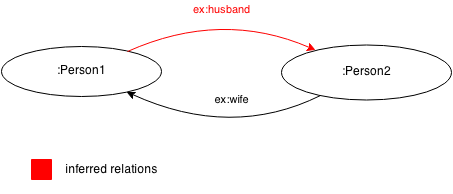
\includegraphics[width=.6\textwidth]{fig/simple-inference}
  \caption{Inference of the husband relation as inverse of the wife relation}
  \captionsetup{font={footnotesize,bf,it}}
  \label{fig:simple-inference}
\end{figure}

Many types of inferences are possible. The inference of the classes of a resource depending on a class hierarchy can be done; the example in figure \ref{fig:inference-hierarchy} shows the usage of the SORELCOM ontology to infer the classes of a resource. Combinations of different inference properties can be used to express complex relations. In figure \ref{fig:complex-inference} inverse and transitive properties together with ranges and domains, are combined to infer knowledge on a small RDF graph.

\begin{figure}[ht]
  \centering
  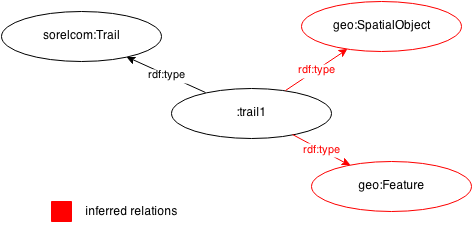
\includegraphics[width=.6\textwidth]{fig/inference-hierarchy}
  \caption{Inference of all the classes of a Trail}
  \captionsetup{font={footnotesize,bf,it}}
  \label{fig:inference-hierarchy}
\end{figure}

\begin{figure}[ht]
  \centering
  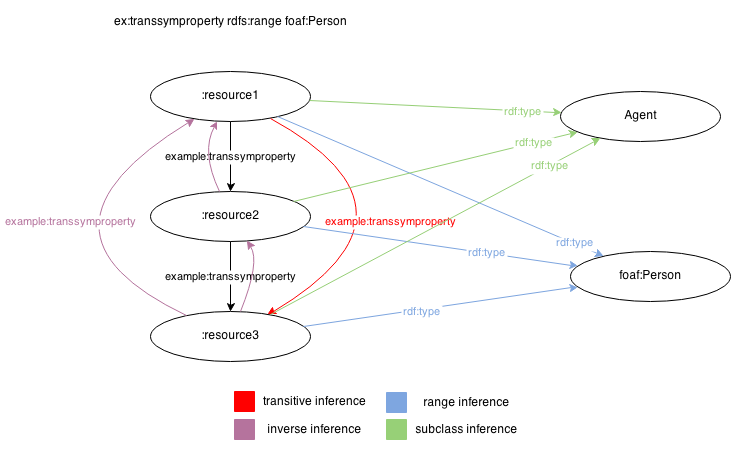
\includegraphics[width=.6\textwidth]{fig/complex-inference}
  \caption{Inference of the husband relation as inverse of the wife relation}
  \captionsetup{font={footnotesize,bf,it}}
  \label{fig:complex-inference}
\end{figure}

Depending on the describing language used, it is possible to create very complex rules, and the inference engine will automatically process all of them. This is one of the biggest advantages over relational database systems where a high amount of relations would need to be defined to encode the complex relations that can be represented in a ontology based system and allows to build complex queries.

\subsubsection{Schema and data separation and reusability}

Ontologies provides mean for reusing other data models, since it is possible to import ontologies into another one. This way, it is possible to use already defined concepts without the need to develop vocabularies for them. One example of this can be found in the SORELCOM vocabulary, where the FOAF, GeoSPARQL, DC and W3C media ontologies are reused.

Besides, this allows separation between the data model and the actual data. In relational database management systems, the structure of the data is physically created on the system itself (for example, a file for each table) and it is not fully supported to import the model of one database to another. When using ontology based databases, the data model is represented by a ontology which can be imported into any data store, thus it is possible to reuse the schema among several different databases.

\subsubsection{Linked Open data}

Ontologies are a tool that facilitate the publishing of Linked Open Data. The inference mechanisms used on these ontologies are not so relevant in this case, however the concepts expressed are crucial. Ontologies allow reusing other vocabularies to express the data model, which is a key point when developing a linked model.

Linked data refers to a set of best practices to publish and interlink structured data for access by both humans and machines via RDF. In order to do this it is necessary to make use of URIs as a real unique identifier, there is no point if a relation that expresses that two persons know each other has a different URI in every dataset. In order to avoid this, well known vocabularies, such as FOAF, and these concepts and relations are uniform among most if not all datasets. This is only possible when using ontology based design, for only ontologies allow this level of reusing.

\section{Design of the central server}\label{sec:serverdesign}

\section{Design of the web application}\label{sec:webappdesign}

\section{Design of the mobile application}\label{sec:mobileappdesign}

\section{Development environment}

The tools and development environment used during the design process have been the following:

\begin{itemize}
\item Prot\'eg\'e-OWL 4.3
\item UML 2
\item Sass 3.8.8
\item Twitter Bootstrap 3.1.1
\end{itemize}

\subsection{Prot\'eg\'e-OWL}

Prot\'eg\'e is an open-source ontology editor and framework for building intelligent systems\cite{protege1}. The traditional architecture of the editor is based on frames \cite{protege2}, however, with the standardization of OWL (see section \ref{sec:owl}) support for this language was added to the framework \cite{protege3}.

The current version of Prot\'eg\'e can be used to edit classes and their characteristics, to access different reasoning engines, to edit and execute queries and rules and to visualize relationships between concepts. The tool has been widely adopted by the Semantic Web ontologists, for all their utilities and because it has been adopted among the W3C recommendations \cite{protege4}.

The tool provides a graphical user interface, which can be seen in figure \ref{fig:protege}. Through this editor, other vocabularies can be imported, in addition to create classes and properties for a new ontology and defining restrictions and relations among them. This tool has been used to create the SORELCOM ontology on the project.

\begin{figure}[ht]
  \centering
  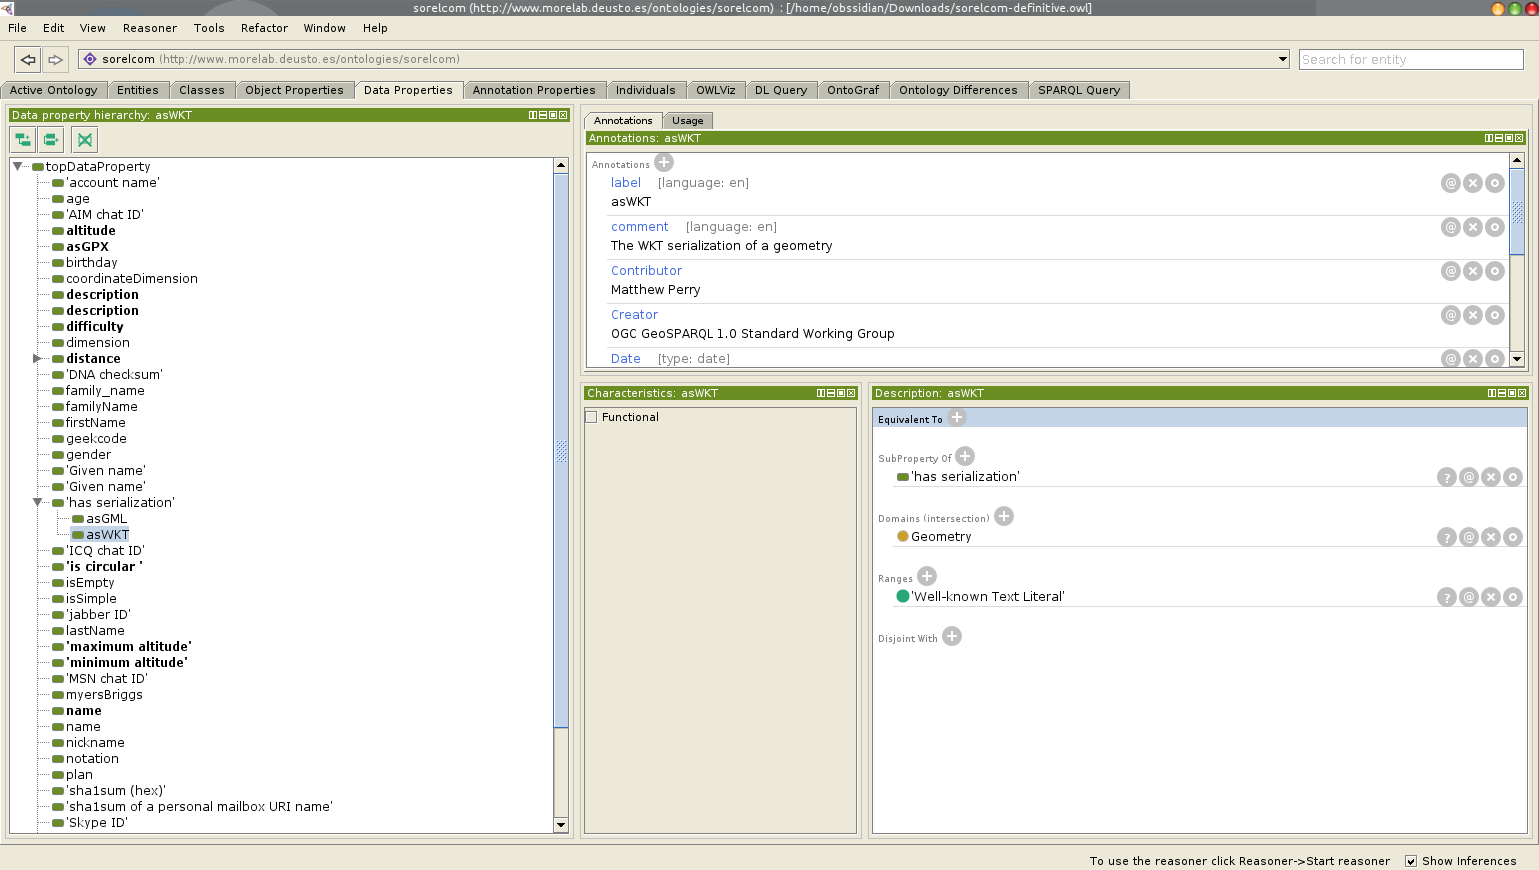
\includegraphics[width=.8\textwidth]{fig/protege}
  \caption{The Prot\'eg\'e OWL ontology editor}
  \captionsetup{font={footnotesize,bf,it}}
  \label{fig:protege}
\end{figure} 

\subsection{UML}

The Unified Modeling Language (UML) is a general-purpose visual modeling language used to specify, visualize, construct and document the artifacts of a software system. It is used to capture decisions and provide understanding of the architecture and class design of the system \cite{uml}. 

UML can be used to capture information about the static design and dynamic behavior of the system and its components through different types of diagram. It is a standard used and accepted worldwide, thanks to which it can be used to expose and interchange information about system designs.

All the component and class diagrams presented in this document have been modeled according to UML standards.

\subsection{SASS}

CSS (Cascading Style Sheet) is a stylesheet language specification used to describe the presentation of documents written in a markup language. It is the technology used to describe the appearance of web pages \cite{css}. SASS \cite{sass} which stands for Syntactically Awesome Style Sheets is a extension and preprocessor for the CSS language which aims to cut on developing times and improve stylesheet maintainability. 

CSS preprocessors have become very popular lately among web developers for various reasons. First, they provide functionality that allows to programatically define styles for a web page instead of just describing, such as variables and functions. Second, these extensions improve code readability and reduce the size of the produced stylesheets. Finally, they follow the principle of DRY (dont repeat yourself), allowing to define the appearance of document without repeating directives. An example of SASS to CSS transformation can be found in figure \ref{fig:sass}.

\begin{figure}[ht]
  \centering
  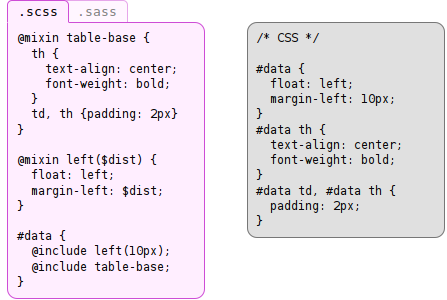
\includegraphics[width=.8\textwidth]{fig/sass}
  \caption{SASS to CSS transformation}
  \captionsetup{font={footnotesize,bf,it}}
  \label{fig:sass}
\end{figure} 

This technology has been used in the project to define the appearance of both the mobile and the web interface.

\subsection{Twitter Bootstrap}

Even with the use of preprocessors, the time it takes to design the appearance of a HTML based application is considerable. In big enough project, specialized designers are employed for the interface design of the application, however on smaller scale projects it has become more usual to use a CSS framework to produce acceptable, if not original, appearances for the user interfaces.

Twitter Boostrap is one of the most, is not the most popular of these frameworks. It provides a set of CSS classes, default styles and JavaScript functions to develop responsive web applications. It has been used in this project to ease the adaptability of the web application interface on all kind of devices.

\chapter{Implementation details}\label{ch:implementation}

This specifies the implementation details of the project, that is, the most significant aspects regarding the coding of the system and its functionalities.

The description of this issues aims at easing possible future enhancements of the system and the maintenance of the code. Some specific aspects of the programming of the code are described and some of the choices made during the implementation process are justified.

\section{Coding style}

There are several well known coding patterns for JavaScript programs. In this project the Google JavaScript Style Guide \cite{googlestyle} has been followed. Below some of the relevant guidelines, and the reasons behind them are listed.

\begin{itemize}
\item Always use \texttt{var} for variable declarations. This is done to avoid the runtime placing the variable in the global context, which can cause overriding of other variables.
\item Variables and functions are named in camelCase, that is, any multi-word name will be written as a single word with the first letter of every additional word in uppercase.
\item Always use semicolons. JS runtimes can run code without the semicolons, however, in some cases they may cause subtle hard to debug errors.
\item Use \texttt{foo.bar = null;} to delete. This is done because the \texttt{delete} operator in JS is slower on many runtime environments. 
\item Use single quotes instead of double quotes. This is a standard across most JS coding styles, for it makes easier to write XML and HTML string, a common task.
\end{itemize}

This are some of the most common guidelines followed, however, there are more rules and small tricks followed, such as caching the array lengths in loops.

\section{Development environment}

This section describes the tools used on the development process. This tools are directly related to the development process but not to the final product.

\subsection{Atom text editor}

Atom is a JavaScript coding oriented configurable text editor developed by GitHub \cite{atom}. It is available for all major operating systems, however it only has prebuilt packages for OS X. Anyway, it provides a repository for Ubuntu OSs which has been used to install it.

The editor is very similar to Sublime Text 2 \cite{sublime} and while Sublime has more years of development and a bigger community behind, Atom offers native NodeJS and Git integration, which declines the balance in favor of Atom for this project. 

It has been used on the project as the sole code editor. An overview of the interface it offers is shown in figure \ref{fig:atom}.

\begin{figure}[ht]
  \centering
  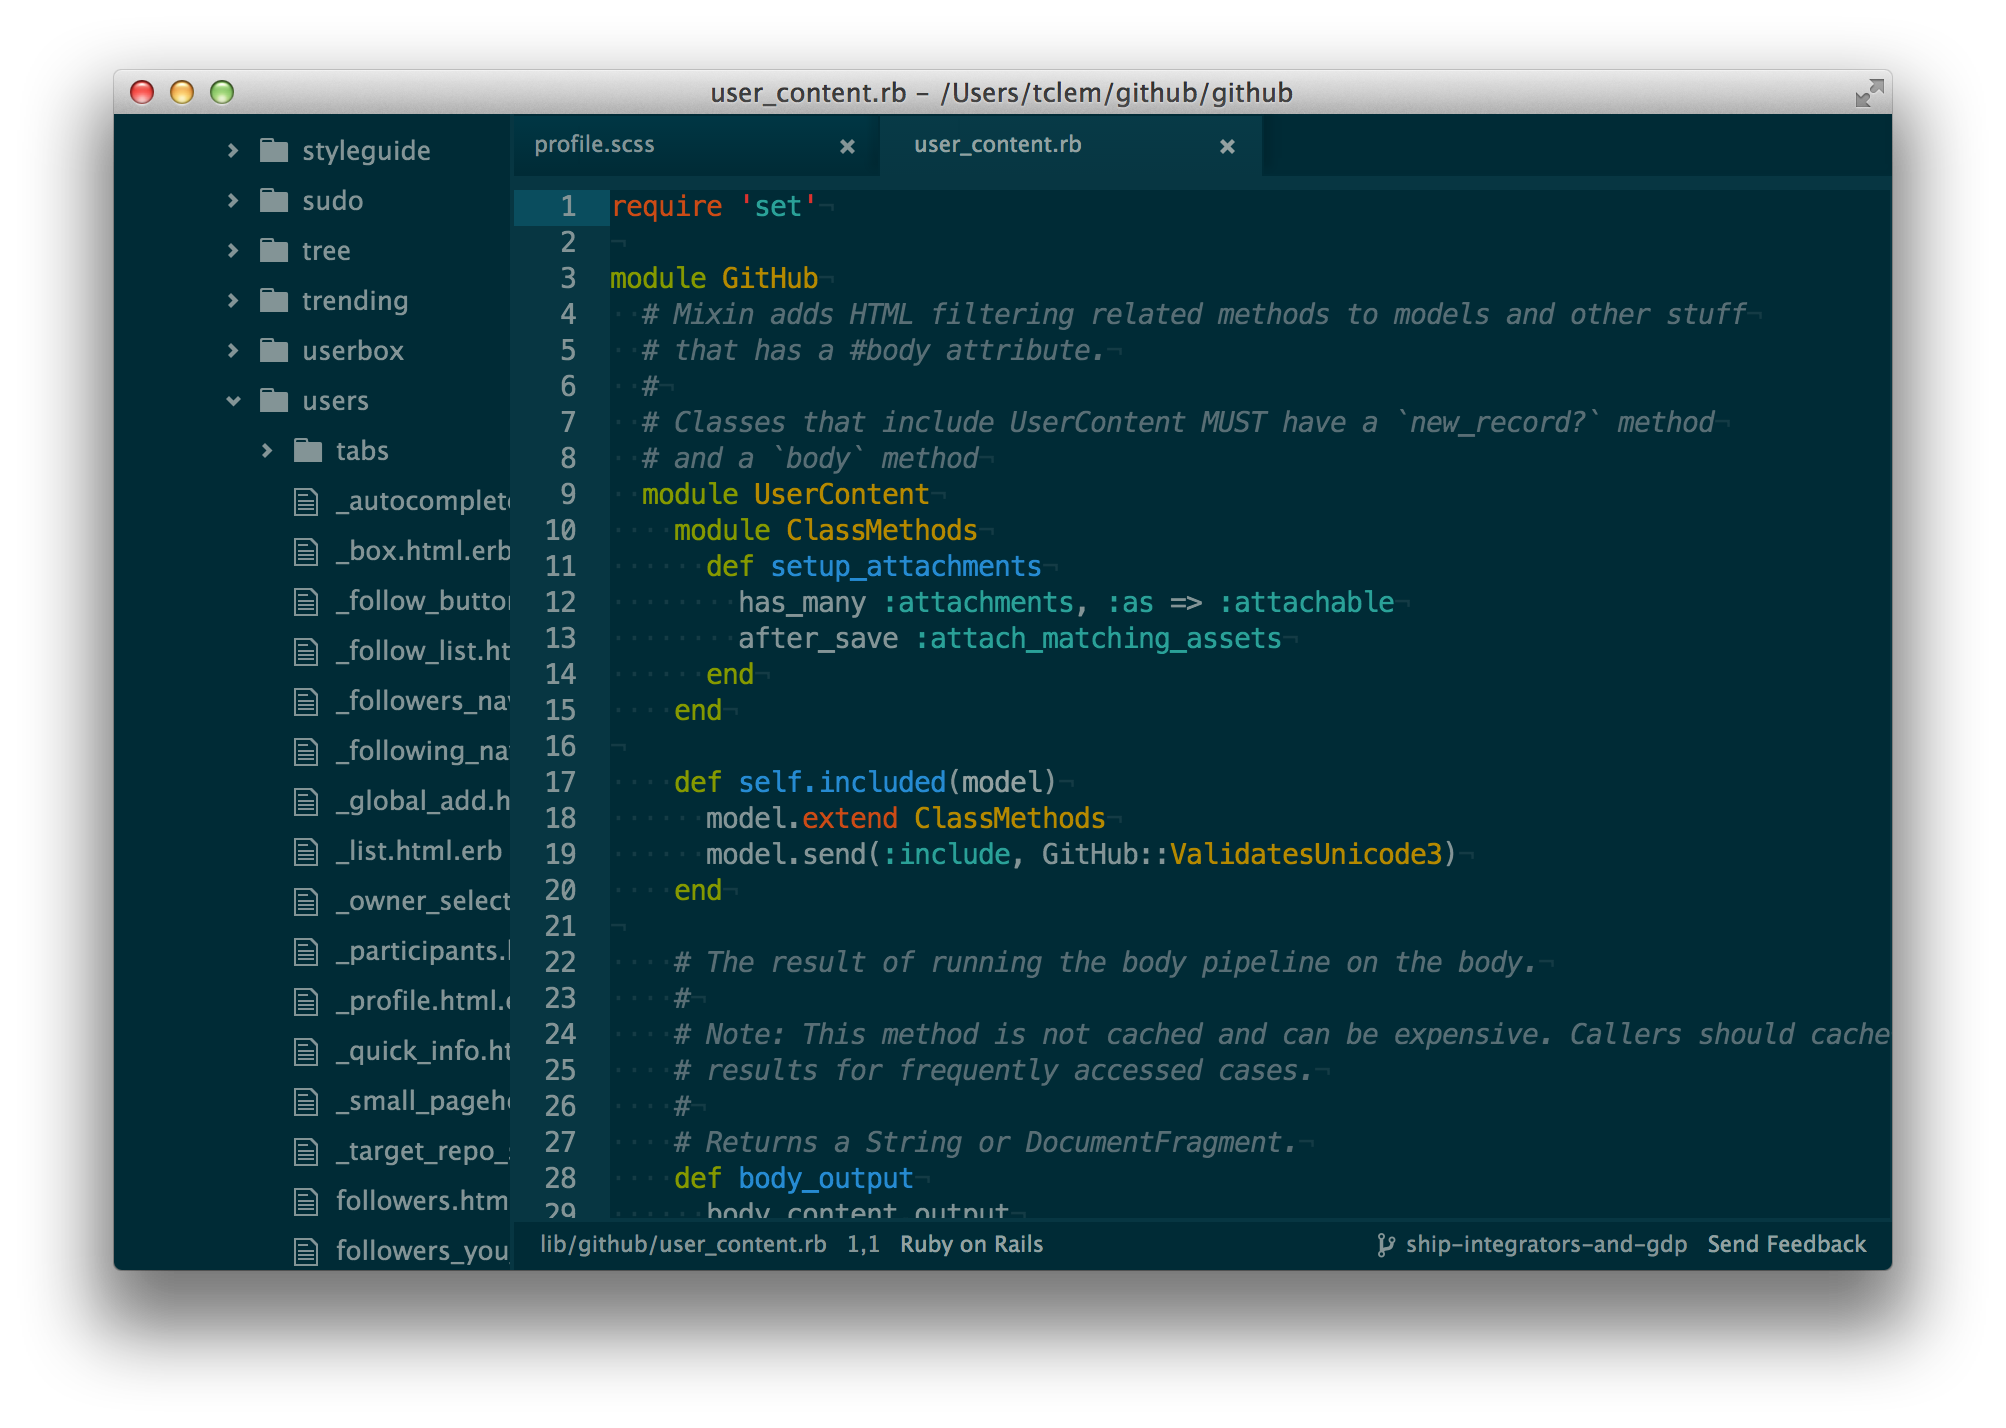
\includegraphics[width=.8\textwidth]{fig/atom}
  \caption{The Atom text editor}
  \captionsetup{font={footnotesize,bf,it}}
  \label{fig:atom}
\end{figure} 

\subsection{Git}

Git \cite{git} is a free and open source distributed version control system with emphasis on speed. 

It has been a very popular tool on open source projects ever since it was developed by Linus Torvalds. It supports the classic functionalities found on all version control systems, in addition to several additional functionalities which make it a superior choice.

The main advantage of GIT is being distributed. Thanks to this it is possible to have local repositories in different machines and synchronize all of them on a single repository, having each local repository keep copies of the whole project.

This project is hosted in the GitHub platform, a free open source project hosting site which supports GIT. A student account, providing three private repositories has been provided by the organization itself.

\subsection{Yeoman}

Yeoman \cite{yo} is a generator ecosystem that helps kickstarting new projects by prescribing best practices and productive tools. 

This tool acts as a command line interface that scaffolds projects, that is, it automatically builds project skeletons which incorporate modern tools. It is based on generators, which specify how an project is created and which technologies are to be used in it.

The development team of Yeoman has created a series of official generators, however, there are several community defined generators that can be used to scaffold different types of projects. This project has used the angular-fullstack generator, used to scaffold a express application which uses AngularJS on the client side.

\subsection{Grunt}

Grunt \cite{grunt} is a JavaScript automation tool that allow to run tasks such as compilation, testing and minification. It becomes incorporated in the majority of the yeoman generators and it is very useful for the deployment tasks of a project, such as code minification and compilation to JavaScript.

It has been used to run the testing, serving and building processes of the project.

\subsection{JSLint}

JSLint \cite{jslint} is a static code analysis tool that promotes and tries to enforce code quality on JavaScript. It works by ensuring that the source code on JavaScript application follows coding rules and best practices.

Grunt can be used to automate the running of JSLint on code changes. In this project, all the source code has been checked using this tool, and no code has been deployed without passing a linter with no errors.

\subsection{Prot\'eg\'e-OWL}

Prot\'eg\'e is an open-source ontology editor and framework for building intelligent systems\cite{protege1}. The traditional architecture of the editor is based on frames \cite{protege2}, however, with the standardization of OWL (see section \ref{sec:owl}) support for this language was added to the framework \cite{protege3}.

The current version of Prot\'eg\'e can be used to edit classes and their characteristics, to access different reasoning engines, to edit and execute queries and rules and to visualize relationships between concepts. The tool has been widely adopted by the Semantic Web ontologists, for all their utilities and because it has been adopted among the W3C recommendations \cite{protege4}.

The tool provides a graphical user interface, which can be seen in figure \ref{fig:protege}. Through this editor, other vocabularies can be imported, in addition to create classes and properties for a new ontology and defining restrictions and relations among them. It has been used to create the SORELCOM ontology on the project.

\begin{figure}[ht]
  \centering
  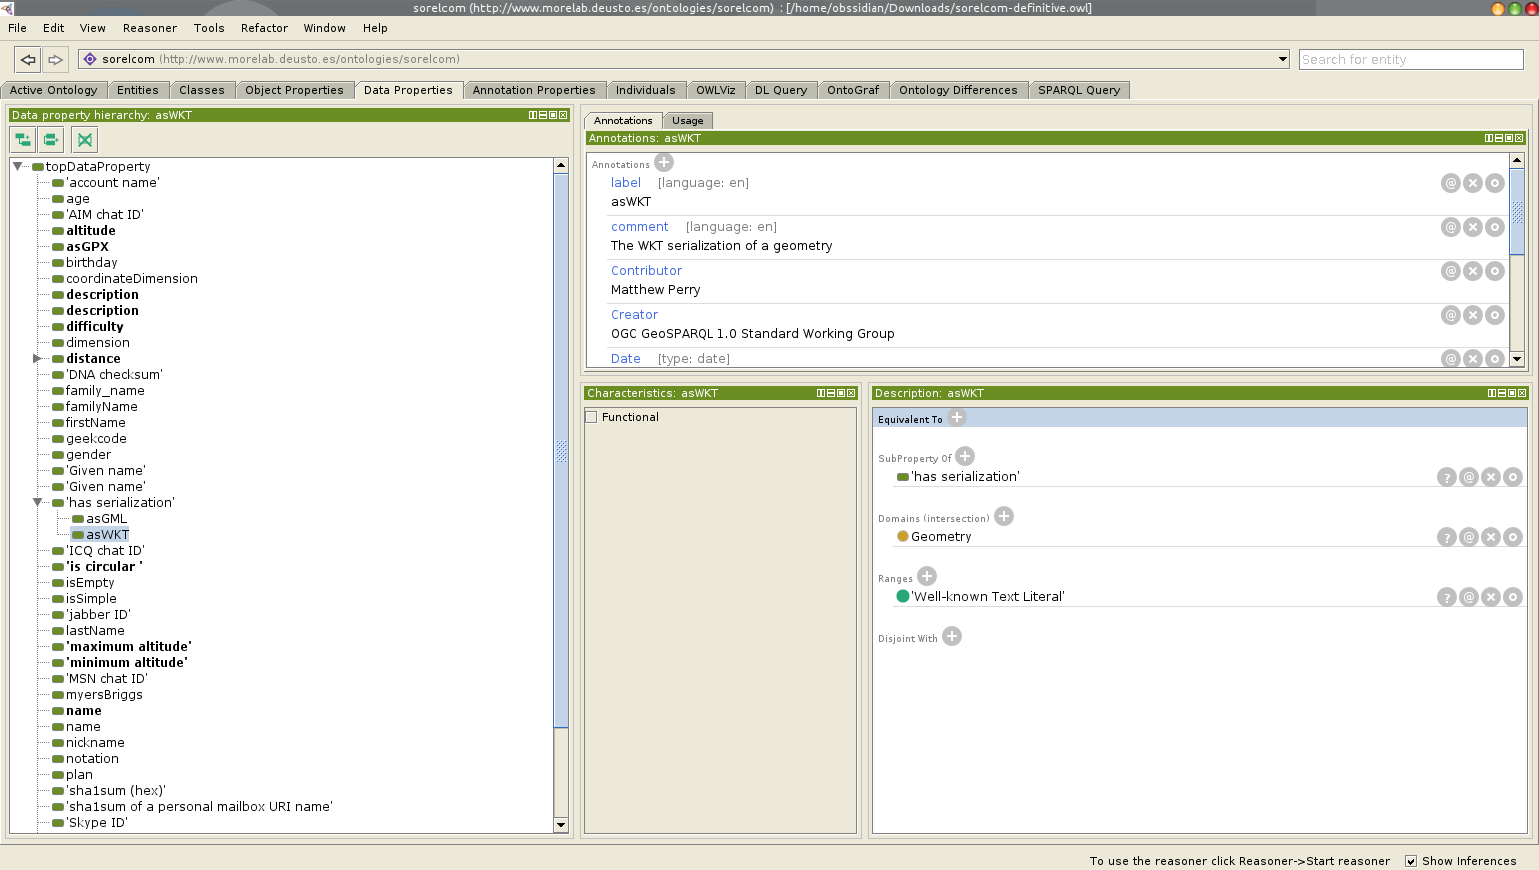
\includegraphics[width=.8\textwidth]{fig/protege}
  \caption{The Prot\'eg\'e OWL ontology editor}
  \captionsetup{font={footnotesize,bf,it}}
  \label{fig:protege}
\end{figure} 

\section{Development of the server}\label{sec:serverdev}

The first step, after the technology research and the design consideration for the development of the project has been the creation of a project using the Yeoman tool. Even though initially only the server is developed, the project skeleton contains a section for the web application, for convenience purposes.

The generator used is the angular-fullstack generator, hosted on \href{https://github.com/DaftMonk/generator-angular-fullstack} and offered though the \textit{generator-angular-fullstack} npm package. 

This command creates the following folder structure.

\begin{description}
\item[app] Contains the code for the web application. Its structure is detailed in section \ref{sec:webappdev}.
\item[lib] Contains the code for the web server.
\item[test] Contains the tests to be run.
\item[node\_modules] Contains the libraries used in the server. It is a mandatory folder in any NodeJS application.
\item [dist] This folder does not exist initially, however, after running the build task it will be populated with the distributable code.
\end{description}

\subsection{NodeJS application structure}

All the code for the server is found inside the \textit{lib} folder. There is still no consensus by the community on which is the file structure that this kind of servers should follow, thus the following structure has been used.

\begin{description}
\item[utils] Utility classes, such as the geographic analyser.
\item[connector] Classes related to the database connector
\item[controllers] Controllers of the server
\item[models] Models of the server 
\item[\textit{routes.js}] Specification of the URLs that the server will route. It is a file, not a folder. 
\end{description}

\subsubsection*{Modules}

External libraries, modules, are used in the Node projects through the keyword \textit{require}. When a module is downloaded through the NPM package manager it is stored in the \textit{node\_modules} folder and can be referenced by a previously defined name. An example of this can be found in listing \ref{lst:require}

\begin{listing}[ht]\centering
  \begin{minipage}{.6\textwidth}
    \begin{minted}[linenos=true,mathescape,gobble=6]{js}
         /** A module called requests is required, an will later be used
         by referencing the variable where it is stored. */
	     var requests = require('requests');
    \end{minted}
  \end{minipage}
  \caption{NodeJS module requiring}\label{lst:require}
\end{listing}

In order to use code defined on files different from the main server, the same mechanism is used. The \textit{require} command obtains an object after running the code on the specified module. The object obtained through the require command is called \texttt{module.exports}. This object is just a dictionary where the function, objects or classes to be exported are appended.

\subsection{Semantic database}

For the server to be able to implement its functionality, it is necessary to first install the database. The storage system to be used is named Parliament, it includes a triple store, a reasoner that supports OWL and GeoSPARQL and a HTTP SPARQL endpoint. 

Two types of packages are offered, which can be found in \href{http://semwebcentral.org/frs/?group_id=159}, the QuickStart bundles and the source files. In this project, a QuickStart bundle for a Linux environment has been used. The advantage of this is that there is no need to install any file to the machine, everything is provided and the database can be running by executing the \textit{StartParliament.sh} file provided.

This bundle uses Jetty, a Java based HTTP server, \textit{jetty.xml} file provided. The default configuration is usually enough, however, since large SPARQL queries are to be done, the form submission size has been changed. The element in listing \ref{lst:jetty} has been added in order to allow the upload of large trails.

\begin{listing}[ht]\centering
  \begin{minipage}{.6\textwidth}
    \begin{minted}[linenos=true,mathescape,gobble=6]{xml}
	     <Call class="java.lang.System" name="setProperty">
	        <Arg>org.mortbay.jetty.Request.maxFormContentSize</Arg>
	        <Arg>500000</Arg>
	     </Call>
    \end{minted}
  \end{minipage}
  \caption{Jetty server configuration}\label{lst:jetty}
\end{listing}

Once the server is configured and running, it can be accessed on the port 8080, using the URL \texttt{http://localhost:8080/parliament}. Doing so offers a interface for the administration and exploration of the triple store. The final step for the installation of the database is configuring the RDF graph on which the information will be saved to generate spatial indexes, which can be done from this interface, as shown in figure \ref{fig:parliament}

\begin{figure}[ht]
  \centering
  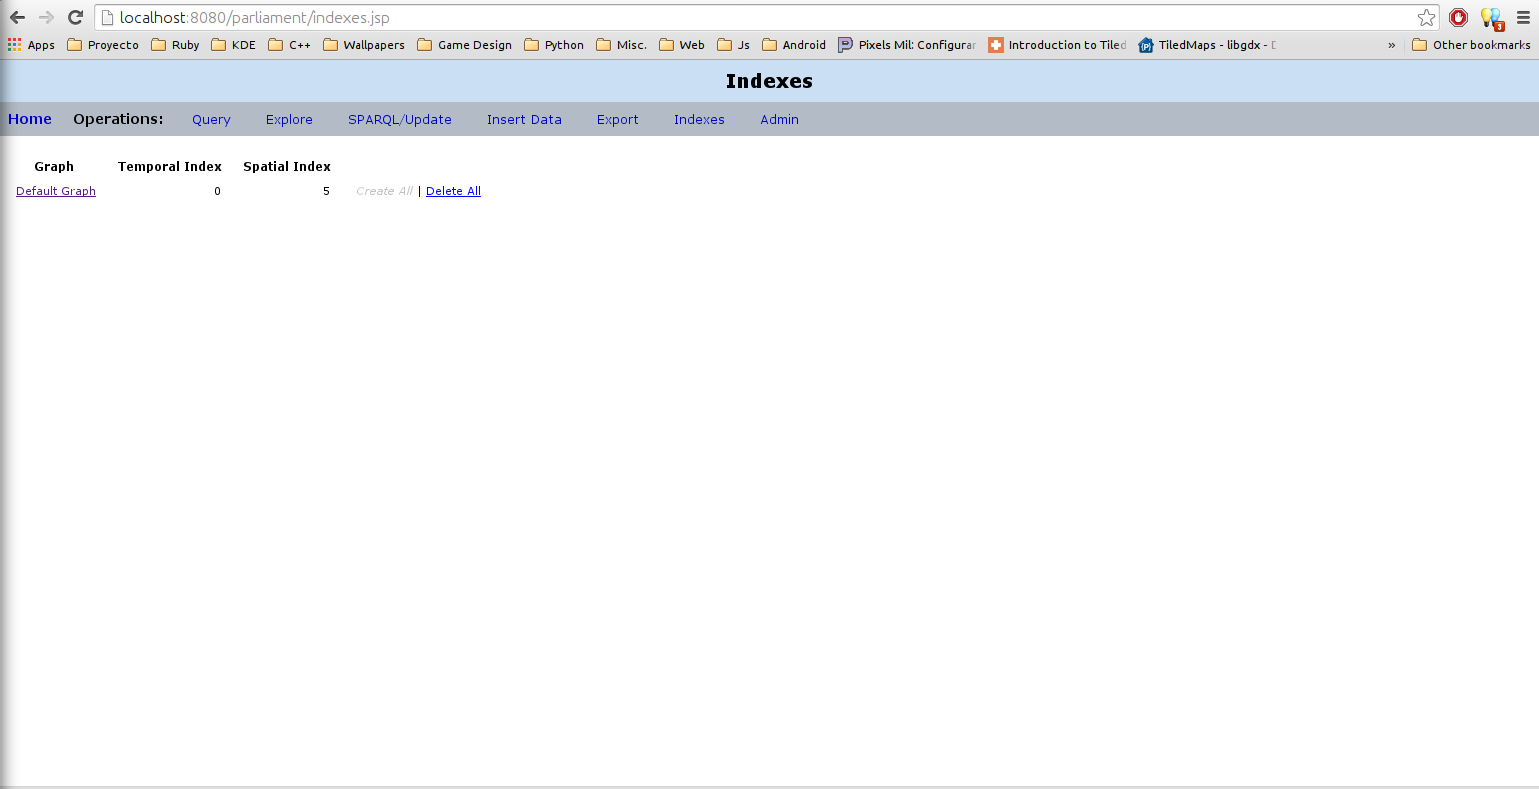
\includegraphics[width=.8\textwidth]{fig/parliament}
  \caption{Web interface of the parliament triple store}
  \captionsetup{font={footnotesize,bf,it}}
  \label{fig:parliament}
\end{figure} 

\subsection{Database connector}

After installing the database, the next step is to develop the database connector. This connector is used to programatically send queries to the data store. Three types of queries will be sent to the endpoint, accessible through the URL \texttt{http:localhost:8080/parliament/sparql}:

\begin{description}
\item[Select] Used to retrieve data from the database. Select queries need to specify a series of bindings, variables that will be retrieved from the database; and a \textit{where} clause which will contain the information actual query. The structure followed is shown on listing \ref{lst:sparql-select}

\begin{listing}[ht]\centering
  \begin{minipage}{.6\textwidth}
    \begin{minted}[linenos=true,mathescape,gobble=6]{text}
	     SELECT ?s ?p ?o #variables to be bound separated by a whitespace
	     WHERE {
	       ?s ?p ?o . 
	     }
    \end{minted}
  \end{minipage}
  \caption{SPARQL Select structure}\label{lst:sparql-select}
\end{listing}

\item[Modify] Used to insert or delete data from the database or both at the same time. SPARQL does not allow to modify existing data, however, it is possible to delete old data and insert the new version in the same query. In order to just insert or delete data, the corresponding part on these queries is omitted. The of the queries is shown in listing \ref{lst:sparql-modify}:

\begin{listing}[ht]\centering
  \begin{minipage}{.6\textwidth}
    \begin{minted}[linenos=true,mathescape,gobble=6]{text}
	     MODIFY
	     DELETE {
	       ?s foaf:name ?name . 
	     }
	     INSERT {
	       ?s foaf:name "new name" . 
	     }
	     WHERE {
	       ?s foaf:name ?name . 
	     }
    \end{minted}
  \end{minipage}
  \caption{SPARQL Modify structure}\label{lst:sparql-modify}
\end{listing}
 
\item[ask] \textit{Ask} queries are used to check if a set of triples exist in the data store or not. They are identical to \textit{Select} queries, however, they just return a boolean value. In this platform they are used to check the uniqueness of resources. The structure of these queries is shown in listing \ref{lst:sparql-ask}:

\begin{listing}[ht]\centering
  \begin{minipage}{.6\textwidth}
    \begin{minted}[linenos=true,mathescape,gobble=6]{text}
	     ASK { ?s ?p ?o }
    \end{minted}
  \end{minipage}
  \caption{SPARQL Modify structure}\label{lst:sparql-ask}
\end{listing}
\end{description}

\subsubsection*{Intermediate Objects}

The controller uses a SPARQL client to communicate with the database, however, before the actual query is sent to the database, it has to be built by the application. The \textit{query maker} that is used by the rest of the application uses a factory to build objects which represent those queries. Then the client will transform these objects into query strings that can be sent to the application.

The reason to use objects instead of directly writing the query is for convenience. It is easier to handle a JavaScript object in the application that a plain string, thus, the server can objects until the moment to send the query through HTTP is reached. These objects are defined in the \textit{connector\_object.js} file, whose contents are shown in listing \ref{lst:sparql-objects}.

\begin{listing}[ht]\centering
  \begin{minipage}{.6\textwidth}
    \begin{minted}[linenos=true,mathescape,gobble=6]{js}
	     function ModifyQuery(del, insert, where){
	       if(del)
	         this.del = del;
	       if(insert)
	         this.insert = insert;
	       if(where)
	         this.where = where;
	     }
	     module.exports.ModifyQuery = ModifyQuery;
	     
	     function ModifyQuery(bindings, where, others){
	     	if(bindings)
	     	  this.bindings = bindings;
	     	if(where)
	     	  this.where = where;
	     	if(others)
	     	  this.others = others;
	     	}
	     module.exports.SelectQuery = SelectQuery;
    \end{minted}
  \end{minipage}
  \caption{The definition of the connector objects}\label{lst:sparql-objects}
\end{listing}

\subsubsection*{Query factory}

The query factory is the class that creates the intermediate objects which will be transformed into the final queries. The implementation of the factory is divided into four classes; the main class containing the methods for creating the general queries and retrieving notes and other three classes containing the methods for creating the query objects that retrieve the defined models from the database.

A good amount of functions has been defined in this cases, one for each possible request and even several for the same request. One example of this methods is shown on listing \ref{lst:factory}, which is used to insert a user in the data store.

\begin{listing}[ht]\centering
  \begin{minipage}{.8\textwidth}
    \begin{minted}[linenos=true,mathescape,gobble=6]{js}
	       this.new = function(args){ 
	         var userid = calculateURI('user', args.name);
	         var avatar = calculateURI('user', args.name, 'foaf_depiction', 'avatar');
	     
	         var where = 'BIND (' + userid + ' AS ?s) . BIND (' + avatar + ' AS ?avatar)';
	         var insert = '?s rdf:label "' + args.name + '" . \
	         ?s rdf:type foaf:Person . \
	         ?s foaf:nick "' + args.name + '" . \
	         ?s foaf:mbox "' + args.email + '" . \
	         ?s foaf:depiction ?avatar . \
	         ?avatar rdf:type sorelcom:Image . \
	         ?avatar sorelcom:storedOn "/images/icon/user.png" . ';
	     
	         return new ModifyQuery(null, insert, where);
	       };
    \end{minted}
  \end{minipage}
  \caption{A query factory method}\label{lst:factory}
\end{listing}

\subsubsection*{SPARQL client}

The SPARQL client is just a regular HTTP client that uses a series of templates to transform the objects created by the factory into actual SPARQL queries. In order to create a SPARQL client, a endpoint to which queries will be thrown and the prefixes that will be perpended to these queries are specified.

This approach allows to use the client on any endpoint, even if it is not part of the system. An example of the query transformation done by the client can be found in listing \ref{lst:transformation}, where a object and the corresponding SPARQL query are shown.

\begin{listing}[ht]\centering
  \begin{minipage}{.6\textwidth}
    \begin{minted}[linenos=true,mathescape,gobble=6]{js}
	       /** Before the transformation process */
	       var query object = {
	         bindings: '?name ?email'
	         where: '?s a foaf:Person . \
	           ?s foaf:name ?name . \
	           ?s foaf:email ?email .';
	         other: 'LIMIT 5' 
	       };
	       /** After the transformation process */
	       var query =
	         'PREFIX foaf: <http://xmlns.com/foaf/spec/> \
	         SELECT ?name ?email \
	         WHERE { \
	           ?s a foaf:Person . \
	           ?s foaf:name ?name . \
	           ?s foaf:email ?email . \
	         } LIMIT 5';
    \end{minted}
  \end{minipage}
  \caption{Query object to SPARQL transformation}\label{lst:transformation}
\end{listing}

In addition to sending requests to the endpoint, the client also has the task of transforming the response of the database into JSON objects to be sent to the requester. The responses of the database is a JSON file following the specification for serializing SPARQL responses as JSON \cite{sparql-json}, the client just takes that serialization and transforms it into a JSON manageable by the application or into a GeoJSON. An example of this transformation is shown in listing \ref{lst:geojsontransform}

\begin{listing}[ht]\centering
  \begin{minipage}{.85\textwidth}
    \begin{minted}[linenos=true,mathescape,gobble=6]{json}
 
	       {
	         "head": { "vars": [ "name" , "geometry" ]
	         } ,
	         "results": { 
	           "bindings": [
	             {
	               "name": { "type": "literal" , "value": "Example feature" } ,
	               "geometry": { 
	                 "type": "literal" , 
	                 "value": "POINT(0 0)", 
	                 "datatype": "http://www.opengis.net/ont/geosparql#wktLiteral" 
	               }
	             } 
	           ]
	         }
	       }

	       {
	         "type": "Feature",
	         "geometry": {
	           "type": "Point"
	           "coordinates": [0, 0]
	         }
	         "properties": {
	           "name": "Example feature"
	         }
	       }
    \end{minted}
  \end{minipage}
  \caption{RDF-JSON to GeoJSON transformation}\label{lst:geojsontransform}
\end{listing}

\subsection{Geography Utilities}

Located in the \textit{util} folder, the geography utilities module provides functionality to analyze features in GeoJSON format, as well as transforming them to WKT in order to store them in RDF.

Most of this analysis consists in obtaining from a set of coordinates parameters such as maximum and minimum height, ascending distance, descending distance or total distance. A method to calculate the distance between two coordinates has been programmed. This method uses a mathematical formula called the \textit{haversine} formula, which can be found on listing \ref{lst:haversine}.

\begin{listing}[ht]\centering
  \begin{minipage}{.9\textwidth}
    \begin{minted}[linenos=true,mathescape,gobble=6]{js}
         function haversine(pt1, pt2){
           var lon1 = pt1[0],
             lat1 = pt1[1],
             lon2 = pt2[0],
             lat2 = pt2[1],
             dLat = numberToRadius(lat2 - lat1),
             dLon = numberToRadius(lon2 - lon1),
             a = Math.pow(Math.sin(dLat/2), 2) + Math.cos(numberToRadius(lat1)) *
             Math.cos(numberToRadius(lat2)) * Math.pow(Math.sin(dLon/2), 2),
             c = 2 * Math.atan2(Math.sqrt(a), Math.sqrt(1 - a));
           return (6371 * c) * 1000;
         }
    \end{minted}
  \end{minipage}
  \caption{JavaScript implementation of the haversine formula}\label{lst:haversine}
\end{listing}

\subsubsection*{Difficulty score}

The difficulty score of a trail is the most relevant data that can be obtained. This difficulty score not only gives an estimation of how hard can it be to a user to follow a route, it can also be used as a deciding factor when trail recommendations have to be done.

In the current iteration of the algorithm, the difficulty score is just based on the slopes on the trail. This value, which ranges from 0 to 100, is calculated by evaluating the different slopes of a trail, grouping them by steepness and comparing the length of each steepness level to the total distance of the trail.

The implementation of this method is shown on listing \ref{lst:score}.

\begin{listing}[ht]\centering
  \begin{minipage}{.7\textwidth}
    \begin{minted}[linenos=true,mathescape,gobble=6]{js}
      var score = 0;
      var meterValue = maxDifficulty/distance;
      for(var i = 0; i < maxSteep; i++){
        var steepValue = k / (maxSteep-1);
        steepValue = ((1 - steepValue) + 1) * steepValue;
        score += steepValue * meterValue * slopes[i];
      }
      return Math.round(score);
    \end{minted}
  \end{minipage}
  \caption{Score calculation algorithm}\label{lst:score}
\end{listing}

This implementation will first calculate a value dividing the maximum difficulty, 100, by the total distance of the trail. This can be seen as the score value for each meter of the trail.

After this, it will start iterating every integer from 0 to the maximum slope calculated, usually 20\%. A proportion for that steep is calculated, in a way that the highest steep gets a bigger value. This value differs more between steep levels the lower the steepness of the levels, that is, the difference between the 0\% slope and the 1\% slope values is greater than the difference between the 19\% slope and the 20\% slope. This allows to differentiate more between trails with low steepness values, which are the most common.

Finally, the distance traversed in that steepness level, multiplied by the proportion of the steepness and the value for each meter, is added to the score. This way, a value that ranges between 0 and a 100 is obtained, being 0 the value of a trail with no slope and 100 the value of a trail with a constant slope of 20\% steepness.

The route calculation could take more parameters into account, such as the type of terrain , however that is left for future versions of the system.

Some factors, however, cannot be added so easily. The most notable of them is the distance. Distance is usually considered a major factor when evaluating how difficult a route is, however, in this case it presents several problems. 

First, distance can vary a lot, one can find trails that cover solely 500m and others that are as long as 100km. Due to this, it is difficult to limit the range of scores when distance is taken as a parameter. Besides, the actual value of the distance is a very subjective factor. For a person that is traversing the trail by foot it may not count as much as for another person that is running through it. Due to this, it has been decided to leave distance outside of the parameters that affect difficulty.

\subsection{Controllers}

The implementation of the controllers is the most trivial task on the development of the server. The job of the controllers is to take the data received on the request, usually a parameter on the URL or an object on the body of the request, extract the data and call a function of the query maker.

Some functions, usually the ones which insert features to the database, need to be analyzed in order to extract the spatial information implicit on their coordinates. In this cases, the controller routes the information to the \texttt{GeographyUtils} class, receives the information and sends it to the database. Figure \ref{fig:controller-sequence} shows a usual control flow for a controller.

\begin{figure}[ht]
  \centering
  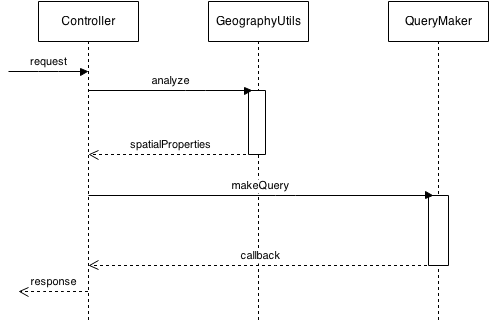
\includegraphics[width=.7\textwidth]{fig/controller-sequence}
  \caption{Sequence diagram for most controller requests}
  \captionsetup{font={footnotesize,bf,it}}
  \label{fig:controller-sequence}
\end{figure} 

Controllers also need to take care of analyzing the response. The Express framework middleware parses the HTTP requests into a JSON object and passes it as a parameter to the controller. In addition, a \textit{response} object is provided to the controller which can be used to send a response. An example is shown in listing \ref{lst:controller}.

\begin{listing}[ht]\centering
  \begin{minipage}{.85\textwidth}
    \begin{minted}[linenos=true,mathescape,gobble=6]{js}
           module.exports.addImage = function(req, res, next){
             if(!req.user)
               return res.send(401);
             
             if(req.body.flowChunkNumber !== req.body.flowTotalChunks)
               return res.send(200); 
               
             short.saveImage(req.files.file, function(err, name){
               if(err) return res.send(500);
               q.Poi.addImage(req.params.id, req.user.name, name, 
                 function(err, data){
                 short.returnOK(err, data, res);
               });
             });
           };
    \end{minted}
  \end{minipage}
  \caption{Controller method for obtaining the trails of a user}\label{lst:controller}
\end{listing}

\subsubsection*{File upload}

Listing \ref{lst:controller} is an example of a controller method that can handle file uploads. Files are uploaded using the \textit{flowjs} \cite{flowjs} library, which sends the files on chunks to the server. 

It is only possible to read the file once all the chunks have arrived. Due to this, it is necessary for the controllers which upload images or videos to the file to check if the chunk of data is actually the last chunk to be sent. In case it is not, then a response acknowledging the client that the data has been received must be sent.

Once the file is fully uploaded, it can be accessed through the \texttt{req.files.file} object. As a sidenote, it is impossible to send more than one file in the same request using this method, however, on the client side it is possible to send multiple files but they will have to be processed one by one on the server.

\subsection{Routes}

The routes of the server are crucial to implement the REST API. In order to define the routes that will be parsed by the server, the Express object offered by the framework must be used. This object exposes five methods to define the URLs that will be read: \textit{get}, \textit{post}, \textit{put}, \textit{delete} and \textit{all}; each of them corresponding to a HTTP method, except for \textit{all} which accepts all methods.

These methods receive two parameters, the first of them is a string or a JavaScript regular expression defining the URL that can be requested and the second argument is the function that is called when a request to that URL is sent.

Listing \ref{lst:routes} defines the URLs from the trail resource of the API. Some of these receive parameters, by specifying a name after a colon; this parameter will be read by the controller on the request object. The same URL can be called from different HTTP operations, however, if no callback is defined for a certain method, the server will send a 404 response.

\begin{listing}[ht]\centering
  \begin{minipage}{.7\textwidth}
    \begin{minted}[linenos=true,mathescape,gobble=6]{js}
           app.get('/api/trails', trails.getList);
           app.post('/api/trails', trails.new);
           app.get('/api/trails/:id', trails.get);
           app.post('/api/trails/:id/images', trails.addImage);
           app.get('/api/trails/:id/images', trails.getImages);
           app.post('/api/trails/:id/post', trails.addPost);
           app.get('/api/trails/:id/post', trails.getPosts);
    \end{minted}
  \end{minipage}
  \caption{API implementation for the trails resource}\label{lst:routes}
\end{listing}

\subsection{Recommendations}

Recommendations, which are currently shown on the profile page of a user, are obtained using SPARQL queries. It is possible to do so thanks to the level of complexity that can be embedded into a single query.

In the first version of the recommendations implemented, the following factors are taken into account:

\begin{itemize}
\item Score of trails
\item Routes traversed by buddies
\item Routes traversed by followed persons
\item Routes added by buddies
\item Routes traversed by followers
\item Distance of the route to the usual location of the user
\end{itemize} 

Listing \ref{lst:recommendation} shows some criteria used on queries to obtain recommendation candidates. It is noteworthy mentioning that these queries are not done independently, they are merged into a single query; in this document they are shown separately for clarity. 

In addition to the filtering shown, the distance of the routes to the usual location of the user is calculated. This is not an actual filtering factor, however, it server to order the candidate routes by their distance to the user. Once this ordering is done, only the few firsts are picked and sent to the user as actual recommendations. 

\begin{listing}[ht]\centering
  \begin{minipage}{.7\textwidth}
    \begin{minted}[linenos=true,mathescape,gobble=6]{sparql}
      SELECT DISTINCT ?trail WHERE {
       ?trail a sorelcom:Trail ; geo:hasGeometry ?tg ;
       sorelcom:difficulty ?difficulty .
       FILTER(abs(?difficulty-50) < 25)
       ?tg geo:asWKT ?twkt .
      }
      
      SELECT DISTINCT ?trail WHERE {
        ?user rdf:label "username"; sorelcom:trailBuddyOf ?buddy .
        ?buddy sorelcom:traversed ?trail .
      }
      
      SELECT DISTINCT ?trail WHERE {
        ?user rdf:label "username"; sorelcom:follows ?followed .
        ?followed sorelcom:maker ?trail .
        ?trail a sorelcom:Trail .
      }
    \end{minted}
  \end{minipage}
  \caption{Criteria for route recommendations in SPARQL queries}\label{lst:recommendation}
\end{listing}

By following this method, the recommendation system can analyse the existing relationships between users. In addition to this, the location of the user is taken into account to a certain point, recommending only nearby routes when there are sufficient candidates. This way, the expressiveness of RDF is combined with spatial queries in order to build a location aware recommendation service.

Usually, recommendation systems use some sort of artificial intelligence, however due to time constraints it has been impossible to implement a more complex recommendation methods. The only possible AI used is the inference engine of the database. Note however, that this is a first version of the final system and there are plans to improve this recommender system with better algorithms and with the addition of more parameters, such as user reviews.

\subsection{Authentication}

The generator used provides a already built authentication service. This service uses the \textit{passport} and \textit{mongoose} NodeJS modules to provide a way of authenticating and storing users.

\textit{Mongoose} is a object database mapper (ODM) that provides a way of modeling models to be used on mongodb databases. It provides a schema based solution for modeling the application data of NodeJS applications.

\textit{Passport} is a flexible authentication middleware for NodeJS. It is based on the concept of \textit{strategy}, which is a way of representing how the users will be authenticated. Different strategies allow using Facebook or Twitter as authentication services, however, in this project only the local strategy based on local database authentication is used.

The generator used provides a \textit{User} modules (in the \textit{models} folder) which contains a nick name, a email and a password. In addition, it comes with a pre built controller for managing users and authenticating them.

In order to take advantage of this, the project uses the provided model and controllers and builds methods for saving and retrieving from the semantic storage on top of them. An example of this is the creation of users, which follows the following procedure:

\begin{enumerate}
\item Retrieve data from the user and save it to the mongodb database
\item Check that the data has been correctly saved
\item Save the user to the triple store
\item Check that the user has been correctly saved
\item If the user is not correctly saved on the triple store, delete it from the mongodb database
\item Return a response according to the result of the operation
\end{enumerate}

\subsection{Real time communication}

The real time communication to be provided has not been implemented in the first phase of the server development. Instead, in order to be able to provide an early prototype of the web application, this functionality has been delayed until it is needed on the development of the mobile application. 

\section{Development of the web application}\label{sec:webappdev}

\subsection{Angular application structure}

The \textit{app} folder of the project contains the code for the web application. It follows a standard Angular folder structure, consisting on the following:

\begin{description}
\item[bower\_components] Third party libraries installed through bower
\item[styles] Style sheets of the application
\item[scripts] JavaScript code of the project
  \begin{description}
  \item[Controllers] Controller source code
  \item[Services] Service source code
  \item[app.js] Application configuration source code 
  \end{description}
\item[vendor] Third party libraries used
\item[views] HTML views of the application
\end{description}

\subsection{Application}

The application file is the first thing to define in a AngularJS project. It is used to create the application itself, to specify which external modules will be used and which will be the routes and views it accepts.

In order to create single page applications, the framework uses the concept of views. When a Angular application is loaded in a browser, its \textit{index.html} file is shown, however, this document usually has a \textit{view} component defined by the \texttt{ng-view} angular directive.

The router of the framework uses the current URL of the browser to embed a different HTML document, called partial view, in the place where the view should be. In this project, the module \textit{ui-router}, an extension of the regular routes has been used.

This module offers enhanced routing capabilities, such as defining nested views. In order to configure this component, the concept of state is used. A state of the application has a URL and a partial view associated. In addition, a controller can be defined to manage that partial view. Some states however, are abstract, meaning that they are only intermediate states with no specific controller and are used to route to nested views. Listing \ref{lst:app} shows the contents of the \textit{app.js} file of the project. Only two state definitions are shown for clarity purposes, since the real number of states is way bigger. 

First, an application is created using the \texttt{angular.module} function, which receive a name for the application and an array with the names of the modules to use. All the source files, even the modules, are included as regular JavaScript scripts in the \textit{index.html} file and the framework will wait for the full loading of the document to execute the code.

Then, a configuration function is used to specify the states that the application will accept. It is also possible to indicate where the browser should be routed when a URL that does not match any state is introduced.

\begin{listing}[ht]\centering
  \begin{minipage}{.85\textwidth}
    \begin{minted}[linenos=true,mathescape,gobble=6]{js}
         var app = angular.module('sorelcomApp', [
           'ngCookies',
           'ngResource',
           'ngSanitize',
           'ngAnimate',
           'ui.bootstrap',
           'ui.validate',
           'ui.router',
           'ui.router.util',
           'leaflet-directive',
           'flow',
           'restangular',
         ]);
          
         app.config(function ($stateProvider, $urlRouterProvider) {
          
          $stateProvider.state('web', {
            abstract: true,
            url: '',
            templateUrl: 'partials/layout.html'
          });
          $stateProvider.state('web.signup', {
            url: '/signup',
            templateUrl: 'partials/signup.html',
            controller: 'SignupCtrl'
           });
         };
    \end{minted}
  \end{minipage}
  \caption{AngularJS application configuration}\label{lst:app}
\end{listing}

\subsection{API}

The API component is used by the rest of the application almost everywhere, thus it is necessary to build it the first. The API acts as a service which comes uses a module called \textit{Restangular} to query the server.

The service offers a object to the rest of components that can be used to retrieve any resource from the API, in addition to some utility functions. The usage of this object, as well as its definition can be found in listing \ref{lst:api}

\begin{listing}[ht]\centering
  \begin{minipage}{.85\textwidth}
    \begin{minted}[linenos=true,mathescape,gobble=6]{js}
          angular.module('sorelcomApp')
            .service('API', function Geo(Restangular) {
            	this.api = Restangular.all('api');
            	
            	this.getTrail = function(id){
            	  return new Trail(this.api.all('trails').one(id))
            	};
            });
    \end{minted}
  \end{minipage}
  \caption{API service class}\label{lst:api}
\end{listing}

This API uses the concept of remote object to provide a means of receiving data from the server without the need of defining a callback each time the API is called. This objects are just containers for data, initially empty. The objects are created by receiving Restangular object which they call immediately after their creation.

A callback is registered to populate the object when the server responds. This callback will call the \texttt{digest} method of the AngularJS root scope, which causes the application to modify the views in order to show the new data.

In addition, a method is provided so that another callback can be registered for when the data arrives to perform additional operations. If the data has already arrived, the callback will be invoked immediately.

Functions of the data, such as getting points of interest and trails can be executed immediately, for they don't depend on the data to be retrieved from the server, only on the provided id.

Listing \ref{lst:remoteobject} shows the implementation of one of such objects.

\begin{listing}[ht]\centering
  \begin{minipage}{.85\textwidth}
    \begin{minted}[linenos=true,mathescape,gobble=6]{js}
          function User(remote){
            var that = this;
            this.prototype = new RemoteObject(remote);
            
            this.remote.get.then(function success(data){
              that.name = data.name;
              that.firstName = data.firstName;
              that.familyName = data.familyName;
              that.homepage = data.homepage;
              that.about = data.about;
              that.ready = true;
              $rootScope.$digest();
            });
            
            this.getTrails = function(callback){
              this.remote.all('trails').getList(callback);
            };
            
          }
    \end{minted}
  \end{minipage}
  \caption{Remote User class}\label{lst:remoteobject}
\end{listing}

\subsection{Accounts}

Most functions of the accounts component are already provided in the application in a similar manner to the server. The \texttt{Auth} and \texttt{Session} services are already created, however, a few changes have been made to the first of them in order to include the functionality needed to require login on some functions.

In addition, the sign up controller and view are provided, and have been left almost unchanged. This controller allows to register a user using a nick name, a email and a password. The only change made has been introducing a double password check before sending the data to the server.

The profile on the other hand is not created during the scaffolding. The profile controller simply downloads the information of the current logged user, using a convenience method of the user resource on the API. This information is displayed in a simple manner in the view and a form is provided to modify it.

When a user signs up it will be immediately redirected to the profile page, in order for it to update the data of his account, such as names and profile picture. It is also possible to see al the activity that the user has done on the platform through this page. Of course, the access is restricted in a way that each user may only access his own profile.

The profile is also used to show recommendations for the user, however, it is not the only place where these can be viewed. If a person is logged in and goes to the homepage, it will be able to see the five trails that are considered most fitting.

\subsection{Web}

The component that has been called "Web" due to its similarity to that of a regular web page consists on four pieces, the home page, the search page and the feature and user views.

\subsubsection*{Home page}

The home page consists on a simple controller that downloads the latest activity on the platform or the user recommendations if the user is signed in. The results are displayed on the page using a peculiar slider.

Since the home page is the first view where a user will arrive when entering the platform, it is important that it is visually appealing. Due to this, the information obtained from the server is not displayed \textit{as is}. 

Since this information will always consist on geographical features which have been created or modified recently, the view shows them on a map. A slider is created which will allow the user to see different maps containing the features obtained. The interaction of these maps has been disabled so that there is no interference with the interaction with the slider. In addition, a event checks when the slide has changed in order to recalculate the size of the map, necessary due to the implementation of the Leaflet library.

\subsubsection*{Search page}

The search page offers a simple interface to make text based search on the server. The controller's only task is to send the query string to the server and to wait for the response to arrive.

Most of the work is done on the view. Since the received data is heterogeneous, users, trails or points of interest may be received; the view must take care of showing the different information of any of the results. This is done using angular directives to hide or show HTML elements. The code for this is shown on listing \ref{lst:search-view}.

\begin{listing}[ht]\centering
  \begin{minipage}{.85\textwidth}
    \begin{minted}[linenos=true,mathescape,gobble=6]{html}
      <main>
       <ul>
        <li ng-repeat="item in searchResults" class="row">
         <a ui-sref="{{makeRef(item)}}" class="col-sm-12 col-xs-12">
          <article>
           <div class="icon col-md-2 col-sm-2 col-xs-2">
            <img ng-src="{{makeIconUrl(item)}}" alt="icon">
           </div>
           <div class="info col-md-9 col-sm-10 col-xs-10">
            <h5>{{item.name}}</h5>
            <div class="details">
             <p ng-if="item.content">{{item.content | limitTo: 40 }}...</p>
             <p ng-if="item.comments">
              <span class="fa fa-comment"> {{item.comments || 0}} </span>
             </p>
             <p ng-if="item.author">
              <span class="fa fa-user">&nbsp;</span> 
              {{item.author}} 
             </p>
            </div>
           </div>
          </article>
         </a>
        </li>
       </ul>
      </main>
    \end{minted}
  \end{minipage}
  \caption{The search view document}\label{lst:search-view}
\end{listing}

Several directives have been used in this (and other) views, including the following:

\begin{description}
\item[\texttt{ng-repeat}] Iterates over a array on the scope and creates a element for each instance.
\item[\texttt{ng-if}] Creates a HTML element when the condition is fulfilled and destroys it when not.
\item[\texttt{ui-sref}] Specifies the state to which the link leads. Provided by the \textit{ui-router} module.
\item[ng-src] Alternative to the \texttt{src} directive which admits brackets (used to indicate angular variables).
\item[\texttt{ng-show} and \texttt{ng-hide}] Hides or shows a html element depending on a condition. Similar to \texttt{ng-if} however it does not create or destroy elements. More efficient when there is a high change ratio on the data. Not used on the shown view.
\end{description}

\subsubsection*{Feature page}

The feature page is just a view showing the details of a certain feature, that is, a point of interest or a trail. The page uses a map to provide a representation of the feature.

To create this map, the \textit{Leaflet-angular-directive} module is used, which allows to embed map following an Angular programming style. It is possible to create a map without using this module, however, for maps which provide solely viewing functionality is is way more convenient to use the module. The usage of this directive is shown in listing \ref{lst:leaflet-angular}.

\begin{listing}[ht]\centering
  \begin{minipage}{.85\textwidth}
    \begin{minted}[linenos=true,mathescape,gobble=6]{html}
      <leaflet width="100%" height="300px" geojson="geojson" id="viewMap"></leaflet>
    \end{minted}
  \end{minipage}
  \caption{Leaflet usage with angular on feature pages}\label{lst:leaflet-angular}
\end{listing}

Images and videos of a feature are shown on this page on a slider. Reviews are also shown on this view, and the uploading of actual posts is implemented through a form which requires a text and a numerical value for the rating.

The information is displayed in a similar manner to the search page, by using angular directives the information that is available for different resources is filtered.

\subsubsection*{User page}

The user page is almost identical to the feature page. The view on the user page does not show any map, for there is no spatial data. One the other side, a navigation menu is provided to view the trails, points of interest, buddies and followers of a user.

An option is provided to follow and add a user as a buddy when the user being viewed is different from the user logged in. In essence it works in the same way as the feature page, all the data is loaded at the start and if the user makes a write action a query is sent to the server.

\subsection{Map}

The Map uses a single general view. This view in addition contains other two nested views, one used for exploring functionalities and the other one offering editing operations.

The general or parent view contains a map which takes the full browser screen. In addition, a sidebar containing the HTML for the nested views. The sidebar can be toggled to be displayed, function that has been implemented completely in CSS.

The controller on the parent view implements only the functionality to show and hide the sidebar. All the map creation is done through a service, shown on listing \ref{lst:map-service}

\begin{listing}[ht]\centering
  \begin{minipage}{.75\textwidth}
    \begin{minted}[linenos=true,mathescape,gobble=6]{js}
     angular.module('sorelcomApp').service('Map', function Map(API){
       var that = this;
       this.initMap = function(id){
         var baseLayers = {
           'OpenStreetMap': L.tileLayer(
             'http://{s}.tile.openstreetmap.org/{z}/{x}/{y}.png',
            )
         };
         this.map = L.map(id, {
           layers: [baseLayers.OpenStreetMap],
           minZoom: 3,
           worldCopyJump: true
         });
         L.control.layers(baseLayers, null, {position: 'topleft'})
           .addTo(this.map);
         this.map.locate({ setView: true, maxZoom: 15 });
       };
     });
    \end{minted}
  \end{minipage}
  \caption{Map service implementation}\label{lst:map-service}
\end{listing}

This service is used by the rest of the explorer and controller services to access the map object and add or manipulate data on it. The controllers on the map component are just gateways that call the methods defined on the services from the views, the actual computation is done on the services. 

\subsubsection*{Explorer}

The explorer does offers a single function. This function is called every time the map is moved or zoomed and queries the server for the features that can be found on the current viewport of the map, represented by its bounding box.

The explorer also generates HTML elements that will be bound to every feature shown in the map. This is used to show the text data (name, description) of a element and to link to the corresponding feature page.

The basic functions of the explorer are shown in listing \ref{lst:explorer}. The \texttt{loadGeoJSON} function takes the results and parses them to create the layers and the popups that will be added to the map.

Trails are only shown when the zoom level is enough to distinguish the routes from points. This is determines by the \texttt{canViewRoutes} function, which check the zoom level of the map. If it is not enough, then the server is asked to return only points of interest.

\begin{listing}[ht]\centering
  \begin{minipage}{.85\textwidth}
    \begin{minted}[linenos=true,mathescape,gobble=6]{js}
      angular.module('sorelcomApp')
       .service('Explorer', function Explorer($rootScope, $q, API, Map, $compile){
    
        this.init = function(){
          Map.map.on('moveend', showView);
        };
    
        function showView(geojson){
          if(!that.categories)
            return;
          var query = { bbox: Map.map.getBounds().toBBoxString() }
          if(!canViewRoutes())
            query.type = 'POI';
     
          that.canceler = $q.defer();
     
          API.withHttpConfig({timeout: that.canceler}).get('within', query).then(
            loadGeoJSON);
        }
      });
    \end{minted}
  \end{minipage}
  \caption{Explorer service implementation}\label{lst:explorer}
\end{listing}

The explorer provides no direct interaction with the user, except for the map zooming and moving event. Instead, the space available on the sidebar is used to show links to the detailed views of each feature and to show a legend of the icons used to represent each element on the map.

\subsubsection*{Editor}

The editor provides several functions related to the manipulation of trails and points of interest.

\begin{description}
\item[Uploading of a GPX file] The upload of GPX files is independent of the map, however, it is accessible in this component because all functions that upload data are grouped on it.

The upload opens a modal which will load a GPX file specified by the user. This GPX is converted to a GeoJSON object to be manipulated by the application and the different features are extracted. Only one can be picked to be created.

Once a feature is picked, a form is used to obtain the relevant data such as the name of the feature or the category if it is a point of interest. This data is sent through a post request to the server.

\item[Drawing a trail] A trail is drawn by adding coordinates to a feature. For this, the editor creates a empty polyline and adds it to a map. After that, a callback is bound to the map click event which adds a coordinate to the polyline. This only happens if the distance between the previous coordinate and the new one is less than 500 meters. The method for doing this is shown on listing \ref{lst:draw}

\begin{listing}[ht]\centering
  \begin{minipage}{.85\textwidth}
    \begin{minted}[linenos=true,mathescape,gobble=6]{js}
      this.startDraw = function(){
          Tooltip.setText('Click on the map to start editing');
          that.editing = L.polyline([]).addTo(Map.map);
          var latlngs = that.editing.getLatLngs();
      
          Map.map.on('click', function(e){
            if(latlngs.length > 0 && e.latlng.distanceTo(latlngs[latlngs.length-1]) > 500) 
              return;
            that.editing.addLatLng(e.latlng);
            that.editing.redraw();
            Tooltip.setText('');
          });
        };
    \end{minted}
  \end{minipage}
  \caption{Map drawing function}\label{lst:draw}
\end{listing}

Stopping the editing of the trail requires only to unbind the click event. One this is done, the editing variable can be transformed into a GeoJSON object and the procedure to follow is the same as when uploading a GPX file.

\item[Marking a point of interest] The process for marking a point of interest is very similar to that of creating a trail. The difference on implementation is that the click callback must be unbound as soon as the click is done. Besides, once the point is marker, the creation dialog is called instantaneously. The implementation of this functionality is shown in listing \ref{lst:mark}.

\begin{listing}[ht]\centering
  \begin{minipage}{.85\textwidth}
    \begin{minted}[linenos=true,mathescape,gobble=6]{js}
      this.markPOI = function(){
        Tooltip.setText('Click on the map to choose location');
        Map.map.on('click', function(e){
          this.stopTask();
          Modal.create(L.marker(e.latlng).toGeoJSON());
        });
      };
    \end{minted}
  \end{minipage}
  \caption{Map point of interest marking function}\label{lst:mark}
\end{listing}

\item[Editing a existing trail] In order to edit a trail, a dialog is prompted to ask the user to import from a GPX file of to download it from the platform. If it is imported from a GPX, the functionality mentioned before is used, however, instread of uploading to the platform, it is shown in the map. If it is downloaded from the platform, a list of trails is obtained using the API and the GeoJSON for one of them is obtained when the user selects it.

In this case the JSON file cannot be directly added into the map. It has to be processed first into a editable polyline, which will be the layer added to the map. This editable polyline is developed as a plugin to the Leaflet library.
\end{description}

\subsubsection*{Editable polyline plugin}

In order to edit trails, a means to do so with a point and click interface is provided through the plugin. The goal is to let the users drag the coordinates of a polyline in order to edit them. The library does not provide any event callback that would allow this in any way, the only draggable elements are markers, which represent single points.

A workaround to providing editable lines is creating a polyline and binding each of its coordinates with a marker that can be dragged. When the marker is dragged, then the coordinates of the line can be updated with the new position. Listing \ref{lst:marker-editable} shows the code for this.

\begin{listing}[ht]\centering
  \begin{minipage}{.7\textwidth}
    \begin{minted}[linenos=true,mathescape,gobble=6]{js}
      this.markerGroup = L.LayerGroup();
      this.markers = [];
      this.latlngs = this.line.getLatLngs();
      for(var i = 0, l = this.latlngs.length; i < l; i++){
        var marker = L.marker(latlngs[i]);
        this.markers.push(marker);
        marker.addTo(this.markerGroup);
        marker.on('dragend', function(e){
          latlngs[markers.indexOf(marker)] = e.latlng;
          line.redraw();
        });
      }
      this.markerGroup.addTo(map);
    \end{minted}
  \end{minipage}
  \caption{Code for adding markers to allow edition of polylines}\label{lst:marker-editable}
\end{listing}

This however does not serve to improve the performance of the editable line. In order to avoid excessive computation time, markers are removed from the map when too many of them are shown at the same time. To do this, a check must be made every time the map is moved or zoomed and if the number of markers is above the maximum, the layer where they are kept is removed. Code for this functionality is shown on listing \ref{lst:marker-check}.

\begin{listing}[ht]\centering
  \begin{minipage}{.75\textwidth}
    \begin{minted}[linenos=true,mathescape,gobble=6]{js}
      var that = this;
      map.on('moveend', function(){
        var count = 0;
        for(var i = 0, l = that.markers.length; i < l; i++){
          if(map.getBound.contains(that.markers[i].getLatLng()){
            count++;
          }
        }
        if(count > maxMarkers && map.hasLayer(that.markerGroup))
          map.removeLayer(that.markerGroup);
        else if(count <= maxMarkers && !map.hasLayer(that.markerGroup))
          map.addLayer(that.markerGroup);
      });
    \end{minted}
  \end{minipage}
  \caption{Code for removing markers to avoid performance issues}\label{lst:marker-check}
\end{listing}

In addition to coordinate dragging, it is necessary to provide functionality to add and remove coordinates from the map. Adding functionality is provided by setting additional markers in the midpoint between each adjacent coordinate pair. When one of these extra markers is dragged, a new coordinate is added to the polyline.

Removing markers on the other hand is simpler. When the user right clicks a marker the corresponding coordinate is removed. This however implies calculating a new midpoint, so that it is still possible to add coordinates in that segment. Pseudo code for these actions are shown on listings \ref{lst:marker-add} and \ref{lst:marker-remove}, the actual code is not shown for clarity purposes.


\begin{listing}[ht]\centering
  \begin{minipage}{.7\textwidth}
    \begin{minted}[linenos=true,mathescape,gobble=6]{js}
      extraMarker.on('dragend', function(e){
        var index = this.extraMarkers.indexOf(e.target) + 1;
        this.latlngs.splice(index, 0, e.latlng);
        this.markerGroup.splice(index, 0, L.marker(e.latlng));
        coordinateAdded(index);
      });
    \end{minted}
  \end{minipage}
  \caption{Add coordinates on a editable line}\label{lst:marker-add}
\end{listing}

\begin{listing}[ht]\centering
  \begin{minipage}{.7\textwidth}
    \begin{minted}[linenos=true,mathescape,gobble=6]{js}
      marker.on('click', function(e){
        var index = this.markers.indexOf(e.target);
        this.latlngs.splice(index, 1);
        coordinateRemoved(index);
      });
    \end{minted}
  \end{minipage}
  \caption{Remove coordinates on a editable line}\label{lst:marker-remove}
\end{listing}

\begin{listing}[ht]\centering
  \begin{minipage}{.7\textwidth}
    \begin{minted}[linenos=true,mathescape,gobble=6]{js}
      function midpoint(latlng1, latlng2){
        return L.latLng((latlng1.lat+latlng2.lat)/2, 
          (latlng1.lng+latlng2.lng)/2);
      };
    \end{minted}
  \end{minipage}
  \caption{Midpoint formula implementation}\label{lst:midpoint}
\end{listing}

The calculation of the middle point of two coordinates is done through the midpoint formula, as shown in listing \ref{lst:midpoint}.

\subsection{Dialogs}

The dialogs component offers means of providing interaction with the user through pop-up boxes, also called modals.

The central class on this component is called the \texttt{Modals} service, used to invoke this dialogs. The \textit{Twitter Boostrap} framework offers functionality and styles to create dialogs and the module \textit{ui-bootstrap} provides Angular services to use them.

This is done through the \textit{\$modal} service, which allows creating a dialog from a defined HTML template and a given controller. The central class of the component uses this service to create different predefined modals. One example of this is shown on listing \ref{lst:modals-shortcut}

\begin{listing}[ht]\centering
  \begin{minipage}{.7\textwidth}
    \begin{minted}[linenos=true,mathescape,gobble=6]{js}
      angular.module('sorelcomApp').service('Modal', function ($modal){
        this.loadGPX = function(){
          var modal = $modal.open({
            templateUrl: 'partials/modals/load.html',
            controller: 'GPXLoadCtrl',
          });
          return modal.result;
        };
      });
      
    \end{minted}
  \end{minipage}
  \caption{Modal invoking shortcuts}\label{lst:modals-shortcut}
\end{listing}

Every method that creates a shortcut returns the \textit{result} of that shortcut. This object is what is denominated a \textit{promise}. Promises are event listeners that listen to a single success of failure from a asynchronous callback. It is possible to define what the promise will do in case of success and what it will do in case of error, in a way similar to callbacks.

By returning the promise object to the controller summoning the modal, it is possible to let it define how the application will behave once the modal finishes its task. This way it is possible to reuse the same code for different functions. For example, the GPX loader modal will return a GeoJSON as a result, which can be used to create a new modal and upload it or can be directly embedded in a map.

The controllers of the modals will return a result using a service called \textit{\$modalInstance} provided by the same Angular module. Using the function \texttt{\$modalInstance.close()} it is possible to return values to whoever is listening the promise. Example \ref{lst:modalinstance} shows how this works.


\begin{listing}[ht]\centering
  \begin{minipage}{.7\textwidth}
    \begin{minted}[linenos=true,mathescape,gobble=6]{js}
      
      $scope.continue = function(){
        $modalInstance.dismiss();
        Modal.create($scope.selected);
      };
      
      $scope.import = function(){
        $modalInstance.close($scope.selected);
      };
      
    \end{minted}
  \end{minipage}
  \caption{Modal closing and communicating functions}\label{lst:modalinstance}
\end{listing}

Most of the implementation of the modals consists in simple functions, mostly to get some data from the user, taken from a form or a button. Most of the implementation of the modals consists on this way of communication, to provide ease of use and reusability.

One modal, however, performs a relatively complex function by itself.

\subsubsection*{GPX loading modal}

The GPX loading modal is in charge of parsing GPX files and extracting the features contained within. In order to do this, a small JavaScript library called \textit{togeojson} is used, which converts from well known geographic encoding formats, such as GPX and KML to a GeoJSON object.

This library will always return a \textit{FeatureCollection} even when only one feature is found. The controller for this modal delegates on a service called \textit{Loader}, which uses this library to generate a GeoJSON and then parses the GeoJSON extracting all of its features.

Once all features are extracted, the user is shown a menu with various maps, each containing one of the features. Once on is selected, the rest of the creation procedure is just standard form data extraction and AJAX calls to the server.

The code for the feature extraction in shown on listing \ref{lst:gpxparse}

\begin{listing}[ht]\centering
  \begin{minipage}{.8\textwidth}
    \begin{minted}[linenos=true,mathescape,gobble=6]{js}
       angular.module('sorelcomApp').service('Loader', function Loader(){
       
        this.extractLayers(text, format) {
          var geojson = toGeoJSON.gpx(jQuery.parseXML(text));
          if(!geojson) return null;
          if(geojson.type === "FeatureCollection"){
            var json = [];
            for(var i = 0, len = geojson.features.length; i < len; i++){
              geojson.features[i].properties.gpx = text;
              json.push(geojson.features[i]);
            }
            return json;
          } else {
            return [geojson];
          }
        }
       });
    \end{minted}
  \end{minipage}
  \caption{Modal closing and communicating functions}\label{lst:gpxparse}
\end{listing}

\section{Development of the Mobile application}

The mobile application reuses many of the classes present on the web application. Thanks to this, the accounts and web components have been reused without any major change. The folder structure of the mobile application is the following:

\begin{description}
\item[app] Contains the application, in a similar way to the server. The contents will be compiled into the \textit{www} folder in order to deploy the application.

\item[www] Contains the scripts, views and styles that the deployed application will use.

\item[test] Contains the tests

\item[platform] Contains the code specific to the platform. In the \textit{src} folder inside is where the Java classes of the application can be found.
\end{description}

The changes for the API have been minimal too, instead of defining a relative URL to make requests to, the URL has been changed to the absolute URL of the server where the application is hosted. The change simply means that instead of having \textit{/api} as the base URL of the API service, this URL will be \textit{apps.morelab.deusto.es/sorelcom/api}.

The functionality offered by the modals has also slightly changed. Since the application will only be executed on the mobile, the dialogs are no longer pop up boxes. This implies slight changes to the views and to the controllers in order to remove the communication functions. However, most of the modals, such as the GPX importing have been removed for there is no need of them in the mobile application.

\subsection{Real time functionality - Server side}

In order for the mobile component to communicate in real time with the server, it is necessary to implement this capability on the web server. This is done using the socket.io library.

It is possible to make Socket.IO application and a Express application work in the same machine and port, however, for this it is necessary to modify the server initialization code, found on the root of the server, in the file \textit{server.js}.

For this it is only needed to require the \textit{socket.io} module and to tell the library object to start listening on the web server, as seen on listing \ref{lst:sioinit}.

\begin{listing}[ht]\centering
  \begin{minipage}{.8\textwidth}
    \begin{minted}[linenos=true,mathescape,gobble=6]{js}
       var io = require('socket.io');
       var express = require('express');
       
       var app = express();
       
       ...
       app.listen(config.port, function () {
         console.log('Express server listening on port %d in %s mode', 
         config.port, app.get('env'));
       });
       var sio = io.listen(app);
       require('./lib/socket/init')(sio);
    \end{minted}
  \end{minipage}
  \caption{Socket.IO server initialization}\label{lst:sioinit}
\end{listing}

The \textit{require} keyword is used after the initialization of the socket in order to define the behavior of the WebSocket once connections arrive. The file specified in the \textit{require} call will be passes the Socket.IO object as a parameter and its code will be executes as in a normal module, with the difference that it will not need to export anything.

\subsubsection{Authentication}

Due to the way the real time functionality works, it is necessary to identify the user using the service. Instead of authenticating the user through the socket, the application uses the session established on the web server. 

In order to do this, there is no need to modify code on the existing web server. A secret key is defined on the configuration files when specifying the behavior of the Express session manager. This secret key, \textit{sorelcom secret} during the development of the project, has to be used to configure Socket.IO authorization mechanisms. The code on listing \ref{lst:socketauth} shows how it has been done.

\begin{listing}[ht]\centering
  \begin{minipage}{.8\textwidth}
    \begin{minted}[linenos=true,mathescape,gobble=6]{js}
       sio.configure(function(){
         sio.set('authorization', passportSocket.authorize({
           key: 'connect.sid',
           secret: 'sorelcom secret', //In lib/config/express
           store: config.sessionStore, //In lib/config/express file
           fail : function(data, accept) { accept(null, false); },
           success: function(data, accept) { accept(null, true); }
         }));
       });
    \end{minted}
  \end{minipage}
  \caption{Socket.IO authorization}\label{lst:socketauth}
\end{listing}

\subsubsection*{Communication protocol}

The communication protocol defined in section \ref{sec:protocol} is implemented mostly on the server. In order to support this protocol, the server uses a subscription mechanism. 

With this mechanism, a connection can subscribe or unsubscribe from a service, such as following a determined trail, at will. This enables to have a undetermined amount of services functioning at the same time, for example, a client may be checking for nearby features and at the same time following trail A and B. Besides, it is relatively easy to implement using JavaScript dictionaries.

When a client connects to the server, a \textit{State} object is created, which will contain the configuration options and the services it is subscribed to. It is noteworthy to mention that the configuration options are global, thus it is not possible to configure trail following distance differently for each trail. The implementation of this class is shown in listing \ref{lst:subscriptions}

\begin{listing}[ht]\centering
  \begin{minipage}{.8\textwidth}
    \begin{minted}[linenos=true,mathescape,gobble=6]{js}
       function State(){
         this.subscriptions = {}
         //Load configuration from the user profile
         this.configs = loadConfiguration(); 
         this.subscribe = function(service){
           if(this.active.service){
             var id = this.subscriptions.service.id;
             this.subscriptions.service = null;
             return id;
           } else {
             this.subscriptions.service = 
               ServiceFactory.createService(service);
             return this.subscriptions.service.id;
           }
         }
         this.setConfig = function(key, value){
           if(this.configs.key)
             this.configs.key = value;
         };
       }
    \end{minted}
  \end{minipage}
  \caption{Subscribing functionality}\label{lst:subscriptions}
\end{listing}

Services follow a pattern similar to regular object oriented interfaces. The idea behind this is to use polymorphism to call the services to which the connection is subscribed. However, JavaScript does not provide support for inheritance out of the box. Still, it is possible to implement polymorphism redefining methods of the prototype of the class. The implementation of the service that implements the trail following service is shown on listing \ref{lst:follow}.

\begin{listing}[ht]\centering
  \begin{minipage}{.8\textwidth}
    \begin{minted}[linenos=true,mathescape,gobble=6]{js}
       function FollowService(trail){
         this.trail = trail;
         this.prototype = new Service('follow ' + trail);
         
         this.prototype.process(coordinates, callback){
           q.isInside(coords, trail, function(err, data){
             if(err) return callback(err);
             if(data.boolean === false) return callback(null, 'FALSE'); 
             q.isLast(trail, function(err, data){
               if(err) return callback(err);
               if(data.boolean === false)
                 return callback(null, 'TRUE');
               callback(null, 'FINISH');
             });
           });
         }
       }
    \end{minted}
  \end{minipage}
  \caption{Trail following service implementation}\label{lst:follow}
\end{listing}

Services implement a function called process, which processes the operations needed to implement the service. The example in listing \ref{lst:follow} queries the database to check if the coordinates are inside of the trail being followed. If they are it checks it the trail has finished. The result is sent through a callback to the main process which will send it as a response to the client.

Due to the way JavaScript works, having a base class in this moment makes no difference with just creating the different services without any inheritance. This approach however, provides a higher extensibility if there is a need to add data to the base class in the future.

The main loop of the socket server implements the functionality needed to read the data. This function checks the command received to perform the different operations. When a subscription is asked it will call the \textit{State} object of the client and subscribe a new service. When coordinates are sent to the server it processes all the services it is subscribed to and sends the responses back to the client.

The data received is a JSON object, thus there is no need to parse the query done by the server, it is already presented as a object to the process. A callback is registered for each command sent by the client and the \textit{argument} members of the data sent are read. The code for the listening process can be found in listing \ref{lst:socket}.

\begin{listing}[ht]\centering
  \begin{minipage}{.8\textwidth}
    \begin{minted}[linenos=true,mathescape,gobble=6]{js}
       sio.on('connection', function(socket){
         var state = new State();
         
         socket.on('nearby', function(){
           var service = state.subscribe('nearby'); 
           socket.emit('OK', service.id);
         });
         socket.on('follow', function(trail){
           var service = state.subscribe('follow ' + trail);
           socket.emit('OK', service.id);
         });
         socket.on('config', function(values){
           for(var key in values){
             state.setConfig(values[key].name, values[key].value);
           }
           socket.emit('OK');
         })
         socket.on('coords', function(coords){
           for(var key in state.subscription){
             var service = state.subscriptions[key];
             service.process([coords.lat, coords.lon], function(err, result){
               if(err) return socket.emit('error', err);
               socket.emit(service.id, result);
             });
           }
         })
       });
    \end{minted}
  \end{minipage}
  \caption{Socket server main process}\label{lst:socket}
\end{listing}

The code subscribes (or unsubscribes) a service on the state of the current connection when the appropriate command is received. When coordinates are received the server loops through all the subscribed services and returns the response when each service is finished processing.

It is important that the server returns the identity of the service every time a new subscription is created or one is deleted. This is used in the client to keep a registry of the services running currently.

There is an additional callback used when the socket is disconnected. It is used to clean all the data accumulated by the user.

\subsection{Real time functionality - Client side}

The client side mobile exclusive functionality are directly related to the real time functionality of the system. This includes tracking nearby features, detecting when the user is deviating from a trail or recording a GPX file.

These functionalities are share something in common: they are continuous and executed during large periods of time. Due to this, it is unreasonable to pretend this functionality to work only when the application is on screen.

In native mobile applications, this kind of batch functions are implemented using service processes. Phonegap, however, does not allow this. Since the applications created using this library are run on a WebView, similar to a browser, JavaScript code can only be executed while the application is open.

There is a workaround for this issue however. Phonegap implements native functionality with something called plugins. These plugins are pieces of native code that can be called from the application itself. Therefore, it is necessary to implement the real time functions of the mobile application as plugins.

This implies coding in Java, the native language for the Android platform. The GPS of the device is acessed natively in this classes to provide the server with the current coordinates of the device, and a Socket.IO Java library is used to communicate this to the server.

Due to this, the application ends up using HTML5 development for interface manipulation and interaction (as well as for the functions borrowed from the web application) and using native code for the background processes.

\subsubsection*{Background service plugin}

Two background services need to be implemented in the application. One of them is used for the recording of coordinates of a trail, the other one for the communication with the server.

The first service is the most straightforward one, it just needs to call the GPS on the device every interval of time. To develop the services, a Phonegap plugin called \textit{Background Service Core Plugin}, found in \href{https://github.com/Red-Folder/bgs-core}, has been used. Through the usage of this plugin, it is possible to develop a Android background service using a simple class structure.

In the Java class representing the service, a \textit{doWork} method has to be written that provides a functionality to be executed at each interval. The interval at which it is executed is specified in the JavaScript code.

In order to use this service with the application, it is necessary to edit the android manifest file. This file presents information about the application to the operating system such as the permissions needed and the services it uses. The lines on listing \ref{lst:manifest} have to be added in order to be able to use the services and the GPS of the device. The services and the permissions are located in different parts of the XML document, however they are put here together for convenience purposes.

\begin{listing}[ht]\centering
  \begin{minipage}{.8\textwidth}
    \begin{minted}[linenos=true,mathescape,gobble=6]{xml}
       <uses-permission android:name="android.permission.ACCESS_FINE_LOCATION" />
       ...
       <service android:name="com.sorelcom.services.TrailRecorder">
          <intent-filter>
             <action android:name="com.sorelcom.services.TrailRecorder" />
          </intent-filter>
       </service>
       <service android:name="com.sorelcom.services.Locator">
          <intent-filter>
             <action android:name="com.sorelcom.services.Locator" />
          </intent-filter>
       </service>
    \end{minted}
  \end{minipage}
  \caption{Android manifest file}\label{lst:manifest}
\end{listing}

The trail recorder service will just pick a point every regular interval of time through the \textit{doWork()} method and will add it to a array, which will be returned to the application as a JSON. This way, once the recording finishes, all the GPX data has been received.

The implementation of this method is shown on listing \ref{lst:recorder}.


\begin{listing}[ht]\centering
  \begin{minipage}{.8\textwidth}
    \begin{minted}[linenos=true,mathescape,gobble=6]{java}
       @Override
       protected JSONObject doWork() {
          Location loc = pointRecorder.getLocation();
          if(loc == null)
            return trail;
          JSONArray coords = new JSONArray();
          coords.put(loc.getLatitude());
          coords.put(loc.getLongitude());
          JSONArray array = trail.getJSONArray( "coordinates");
          array.put(coords);
          return trail;
       }
    \end{minted}
  \end{minipage}
  \caption{Recorder service implementation}\label{lst:recorder}
\end{listing}

The \textit{PointRecorder} appearing in the recorder service is different from the one on the design specified in section \ref{sec:mobileappdesign} on chapter \ref{ch:design}. The one used on the service is just a utility class that encapsulates the functionality of the \textit{LocationManager} class used in android to retrieve the current location of the user. 

This point recorder uses the created services as a android context to gain access to the GPS of the device. The code for creating point recorders is shown on listing \ref{lst:pointrecorder}. Since the GPS device may be temporarily disabled, the location manager records the last location and sends it to the user as a fall-back if there is no GPS.

\begin{listing}[ht]\centering
  \begin{minipage}{.8\textwidth}
    \begin{minted}[linenos=true,mathescape,gobble=6]{java}
       public class PointRecorder{
         LocationManager manager;
         Location lastLocation;
       
         public PointRecorder(Context context){
           manager = (LocationManager) context
               .getSystemService(LOCATION_SERVICE);
         }
         
         public Location getLocation(){
           if(locationManager
               .isProviderEnabled(LocationManager.GPS_PROVIDER)){
             lastLocation = locationManager
                 .getLastKnownLocation(LocationManager.GPS_PROVIDER);    
           }
           return lastLocation;
         }
       }
    \end{minted}
  \end{minipage}
  \caption{Recorder service implementation}\label{lst:pointrecorder}
\end{listing}

The last service to implement is the location tracker service. This service has to communicate with the Socket.IO server, for which a client library is needed. A Java implementation of the Socket.IO library has been used for the creation of this functionality. This library can be found in \href{https://github.com/Gottox/socket.io-java-client}. The service is very similar to the tracker service regarding implementation, however, it uses the \textit{doWork()} and configuration methods to communicate information to a class implementing the protocol on the client side. The code of this class is shown on listing \ref{lst:socketclient}.

\begin{listing}[ht]\centering
  \begin{minipage}{.8\textwidth}
    \begin{minted}[linenos=true,mathescape,gobble=6]{java}
       public class SocketIOClient{
         SocketIO socket;      
         ConnectionStatus status;
        
         public SocketIOClient(){
           socket = new SocketIO("http://apps.morelab.deusto.es/sorelcom");
           ConnectionStatus status = new ConnectionStatus();
         }
         public void start(){
           socket.connect(status.callback);
         }
         public void sendCoordinates(Location loc){
           JSONObject object = new JSONObject();
           object.put("lat", loc.getLatitude());
           object.put("lon", loc.getLongitude());
           socket.emit("coords", object);
         }         
         public void addService(String name){
           status.toggleService(name);
         }
       }
    \end{minted}
  \end{minipage}
  \caption{Socket communication client}\label{lst:socketclient}
\end{listing}

The client implementation works in a identical way to the server. When the user want to subscribe to a new service, the socket subscribes adds it to a list of services. The difference is that instead of having a function encoded to a service, the client services will subscribe a callback to the IOCallback object used on the socket. Note that the services mentioned here are different from the android \textit{Services}.

When a new service is added, the a new callback is subscribed to the socket, as shown in listing \ref{lst:clientservice}.

\begin{listing}[ht]\centering
  \begin{minipage}{.8\textwidth}
    \begin{minted}[linenos=true,mathescape,gobble=6]{java}
       Map<String, IOService> active;
       
       public ConnectionStatus(){
         active = new Map<String, IOService>();
         final ConnectionStatus st = this;
         callback = new IOCallback(){
           @Override
           public void on(String event, IOAcknowledge ack, Object... args) {
              if(st.active.contains(event))
                active.get(event).process(args);
           }
         }
       }
       public toogleSubscription(name){
         if(active.contains(name)){
           active.get(name).destroy();
         } else {
           active.put(name, ServiceFactory.createService(service));
         }
       };
    \end{minted}
  \end{minipage}
  \caption{Service subscriptions and server message reading}\label{lst:clientservice}
\end{listing}


Most of the code of the document is not shown on this section, however, the design specifies how the control flow works among the different classes on figure \ref{fig:plugin-flow} on page \pageref{fig:plugin-flow}.

\subsubsection*{Application-to-service communication}

The interface needs to provide a way to communicate the user with the services in order to access this functionality. This includes allowing a user to start or stop following a trail, activating or deactivating the location tracking process and starting to record a GPX.

This is all done through the AngularJS services specified for the mobile client (see \ref{fig:mobile-diagram} on page \pageref{fig:mobile-diagram}). The services, programmed in the native language, are accessed on the JavaScript code through the use of the Cordova library. The code for creating a service can be found on \ref{lst:makeservice}. This code is called when the Angular service handling the Android service is created.

\begin{listing}[ht]\centering
  \begin{minipage}{.8\textwidth}
    \begin{minted}[linenos=true,mathescape,gobble=6]{js}
       var factory =cordova.require(
        'com.red_folder.phonegap.plugin.backgroundservice.BackgroundService');
       var trailService = factory.create('com.sorelcom.services.TrailRecorder');
    \end{minted}
  \end{minipage}
  \caption{Android service creation from the application}\label{lst:makeservice}
\end{listing}

Once the service is started, the application can access a uniform API to set intervals on which the code of the service will be run and to receive results. For this, the application should register for updates on the service. This will cause the application to receive a JSON object, returned by the doWork() method on the service, every interval of time specified.

In addition, the service can be stopped by disabling it's timer. Once this is done, a JSON object corresponding to the result of the last interval is returned. This is used on the GPX tracker to obtain the finished route once the user decides to stop recording.

In addition, the service can receive configuration options through another method on the API. This configuration methods are used on the Location tracker to enable and disable different services, that is, configuration is changed when the user activates or deactivates the nearby feature discovery or when the user decided to start or stop tracking a service. Initialization of the trail recording service is shown on listing \ref{lst:startservice}.

\begin{listing}[ht]\centering
  \begin{minipage}{.8\textwidth}
    \begin{minted}[linenos=true,mathescape,gobble=6]{js}
       trailService.getStatus(function(status){
         startService(status)
       });
       
       function startService(status) {
          if (status.ServiceRunning) {
             enableTimer(status);
          } else {
             myService.startService(function(data){
               enableTimer(data)
             });
          }
       }
    \end{minted}
  \end{minipage}
  \caption{Trail recording service starting from the application}\label{lst:startservice}
\end{listing}

Once the service is started, it is possible to enable a timer interval. Functions for starting the trail recorder timer and receiving data from the service are shown on listing \ref{lst:starttimer}

\begin{listing}[ht]\centering
  \begin{minipage}{.8\textwidth}
    \begin{minted}[linenos=true,mathescape,gobble=6]{js}
       function enableTimer(status) {
          if (status.TimerEnabled) {
             registerForUpdates(status);
          } else {
             this.trail = [];
             myService.enableTimer(recordInterval, function(data){
               registerForUpdates(data)
             });
          }
       }
       
       function registerForUpdates(status) {
          if (!status.RegisteredForUpdates) {
             myService.registerForUpdates(function(data){
               if(data.latestResult != null){
                 //Push last coordinates to the trail
                 this.trail.push(data.latestResult);
               }
             });
          }
       }
    \end{minted}
  \end{minipage}
  \caption{Trail recording timer start and data reception implementation}\label{lst:starttimer}
\end{listing}

\section{Application functionality}

The implementation of the rest of the application is almost identical to that of the web application. The work necessary is just a few modifications on the views, eliminating the dialog communication functionality from the modal controllers and creating the new controllers to communicate with the plugins.

In addition, the functionality to create a geolocated note must be created. This function however can be done using only Phonegap provided functions. The reason for creating background services is just providing the user with a functionality that persists when the phone is blocked. Since posting a note is done in a single point in time, while the application is on screen, there is no need to create a service for this.

Instead, the Phonegap geolocation plugin is used. This plugin accesses the GPS device and provides a single coordinate set representing the current position of the user, perfect for the note posting functionality. The code to obtain this coordinates is shown on listing \ref{lst:phonegap-location}.

\begin{listing}[ht]\centering
  \begin{minipage}{.8\textwidth}
    \begin{minted}[linenos=true,mathescape,gobble=6]{js}
       navigator.geolocation.getCurrentPosition(function(position){
         note.addPosition(
           position.latitude,  
           position.longitude, 
           position.coords.altitude || 0);
       });
    \end{minted}
  \end{minipage}
  \caption{Location retrieval using Phonegap}\label{lst:phonegap-location}
\end{listing}

Once the location is obtained, the note will just be sent as a GeoJSON to the server through a HTTP POST request to the REST API. This is the only functionality noteworthy on the server (besides the services), the rest is a slight modification of the web application functionality.
\chapter{Testing}\label{ch:testing}

\section{Overview}

During the project, several tests have been carried out in order to guarantee the quality of the code and minimizing the amount of errors that may appear in the development process. This chapter describes the tests carried out through the project.

The following sections are described in the chapter:

\begin{description}
\item[Test plan] Different kind of tests and procedures to be carried out on the project.
\item[Special test cases] Special cases that require more intensive or just different testing.
\end{description}

\section{Test plan}

In order to test the application, different types of tests have been defined. The following test types have been carried out through the project.

\begin{description}
\item[Unit tests] Units tests are test procedures that verify the functionality at of a specific section of code, such as a class.

\item[Integration tests] Tests are carried the correct integration of different kinds of components. These tests have been carried out iteratively, checking the integration of a component every time it is added.

\item[Installation tests] Tests to check that the installation of a certain component has been carried out correctly.

\item[Special test cases] Test carried out in cases where no other tests can be carried.
\end{description}

\subsection{Unit tests}

The units test carried on the project usually have as a goal the verification of the implemented functionality when confronted with both regular values and extreme values or special cases. The tests are focused on the following aspects:

\begin{itemize}
\item \textit{Array indexes:} Checking if loops and other functions don't try and access values outside of the array bounds. This is important is JavaScript programming because no index out of bounds exception will be thrown, but a undefined value will be returned.

\item \textit{Undefined and null variables:} Specially in condition checking it is important to check how variables behave. This is because in some browser a undefined, a null and a false are completely equivalent while in others no. Besides, some runtimes provide undefined values when others provide null values.

\item \textit{Type casting:} On dynamic typed languages it is important to check cases sensible to the automated type casting done by the runtime. For example, when checking equality using a "==" instead of a "===" operator, a string may be cast to number. These errors are usually hard to find a debug, so it is important to check for them.

\item \textit{String building:} String building is a very common operation in this project, due to the need of creating SPARQL queries. Thus, it is vital to check operations that perform this type of task.

\item \textit{Iterations, conditions and callbacks:} Any project needs to check that the control flow is correct. In event oriented environment which make exhaustive use of callback functions it takes a higher importance due to the rise on the control flow complexity.
\end{itemize}

The unit test for each component has been carried out as the development of the component was carried out. This is done to detect early errors that may affect other parts of the component.

However, due to the heavy amount of communication carried through the project, the amount of unit test has been relatively small, and integration tests have taken a bigger role.

In order to carry these test units, two tools have been used:

\subsection{Integration tests}

Integration tests check that the integration of the different components on the system is correct. These test check that the APIs offered by these components are usable by other parts of the system, but not only this, they also check that the errors on one side do not affect the others.

The integration tests carried can be divided in the following parts:

\begin{itemize}
\item \textit{Database connector:} The database is a central piece of the application, thus it is important to check that the communication of the server with it is correct. These tests include checking that the server can handle database errors, that the data sent to the database is valid and that the responses of the database can be always parsed correctly.

\item \textit{API:} Testing the correctness of the API functions is important since it is used as a central point of communication. As usual this implies checking the validity of data received and the extreme cases. In addition, the connectors on the clients also need testing, in order to validate that they query the correct resources of the database.

\item \textit{Socket communication:} The socket server is prone to error, for there are many operations involved, such as connection establishing and destroying. Authorization, session data storage and communication in itself must be checked, both in the client and in the server.
\item 
\end{itemize}

\subsection{Installation tests}

The installation tests aim to verify the installation of one or more components of the project. This means checking the validity of the installation of the database. This is needed because the data storage system includes uncommon functionality, that is, a reasoner, a triple store and a endpoint.

The following tests have been carried out:

\begin{itemize}
\item \textit{SPARQL endpoint:} The endpoint has to accept queries and answer in the desired format in order to pass these tests. In addition, it must accept the different SPARQL protocols to be used on the project.

\item \textit{Reasoner:} The correct functioning of the reasoner, that is, the capability of the system to generate knowledge from the provided triples must be validated.
\end{itemize}

Some of these tests, such as the SPARQL endpoint can be carried at the start of the project, however, they require hand made testing. This means manually writing SPARQL queries to the database to check it works.

Testing the reasoner, on the other side, cannot be done so early. First it is needed to develop the ontology and create the spatial indexes of the database. Once this is done it is possible to elaborate spatial queries and to insert data to check the functioning of the inference engine.

\section{Special test cases}

The test plan comprehends different kinds of standard tests that are carried out in any project. Some tests, however, cannot be automated so easily and require manual work to check their validity. The following test have been considered special cases:

\subsection{Ontology}
 
When a ontology is not well designed errors may arise during the inference process. A typical example of this is inferring that a resource belongs to two different classes that should be disjoint.

In order to test the validity of the ontology, data has been inserted to the storage system and then the generated triples have been analyzed. Analyzing the triples means just looking at them and determining if the results obtained conform with what was expected on the ontology.

This approach however has a issue. It is very difficulty to check all the cases that may cause problems, thus, common sense and careful analysis are important when carrying out these tests. Still, it can be guaranteed that most of the cases are checked and that all major errors are solved. 

\subsection{Trail recording and locator service}

While it is possible to test the correct functioning of the communication protocol and the validity of server and client side functions, it cannot be certainly said that the services work correctly until they have been tested by a user.

This means that even if the platform can query the server for nearby points of interest and read the response, there is no guarantee that the functionality provided is actually the desired one. In these cases, a certain amount of real data is needed to check that the provided service is the one required.

This is usually done by alpha and beta testing, however, before these phases can begin in the project a small amount of field tests have been carried. This test consist in simply uploading a small amount of test data to the server and using the mobile application on a real environment.

\subsection{User interaction}

The interface of, the means of user interaction, the application need some testing too, as well as the logical components. This however does not imply testing for the validity of the interface, but for other features such as ease of use and learning.

In order to do this, external testing and feedback is needed. It is impossible for the interface to be tested by the developers since they are biased, they know exactly what the functionality is, thus they will find it very hard to signal the unintuitive features of the interface.

Due to this, this testing has been delayed to the beta phase of the project.
\chapter{User guide}\label{ch:user-guide}
\chapter{Conclusions and future lines of work}\label{ch:conclusions}

\section{Overview}

This chapter compiles, as a conclusion, the opinions of the work group after the realization of the \textit{SORELCOM} project, showing their impressions on the work done and taking into account the contributions its development has made both at a personal and professional level.

\section{Goals achieved}

After following the development process, it can be stated that all the goals listed in section \ref{sec:goals} have been accomplished:

\begin{itemize}
\item A location-aware service has been created, which takes advantage of the advantages that the semantic web offers (linked-data, inferences, etc.). This service is offered to the users through a GPS community and a mobile service.

\item Several Linked Open Data vocabularies have been used on the definition of the \textit{SORELCOM} data model, thus allowing he publication of data as Linked Open Data. 

\item A model for the representation of trails and points of interest has been created. In addition, this model supports point of interest categories, compatible with OpenStreetMaps taxonomies and Geolocated Notes.

\item A method for calculating the score of a route has been created, thus giving the possibilities of evaluation. The means of corrections are provided through a trail editor interface.

\item The tools for a GPS community have been created. Whether a community is built around them, only time will tell.

\end{itemize}

\section{Considerations}

The SORELCOM project has been an amazing learning experience. Through the duration of the project I have learned a lot about many things, however, the most prominent or interesting of them has been the Semantic Web. During the whole degree, the only data modeling technique we are shown is relational database modeling, thus ontology based modeling has been exciting surprise. However, the ideas and the purpose behind the Semantic Web and Linked Open Data, the idea of building a web for machines with integrated data, a better web, is what has made this concept of semantic web most interesting for me. At first I was skeptic about this technology, due to the complexities it brought to the project and the low understanding I had of it, however with time and learning I have found that I really like the ideas behind the Semantic Web and it is a field I would like to explore more in depth.  

In addition, the possibility of developing a web server using NodeJS has been something I have appreciated. I knew of this technology beforehand, however, I n ever found a opportunity to use it on a real project. Having the possibility of choosing the technology to use in the development gave me a great opportunity to finally use this tool on a decent sized project. This project has not only given me the chance of learning of The Semantic Web, I have also been able to use a technology I had been wishing to try for a while and I have learned a lot about state of the art web and mobile development tools. Not only this, but due to the involvement I've had with web development technologies and tools for the duration of the project, I have learned a lot about the web itself and about the current trends and tendencies on this field. 

Another technology that I have learned during the project is SocketIO. The technological implications may not have been so great, since during the degree we students learn to program TCP sockets, however the possibilities that this library opens are many. The ability to establish real time communication on web pages, among other environments, brings up a lot of possibilities and a lot of ideas for new project.

GeoJSON, RDF, Express, SocketIO, Phonegap, AngularJS, SASS, etc. Many technologies have been used through the projects, which I've had to learn. This has been a big time investment, however, it has also improved my learning capability and my skills as a computer engineer and programmer overall.

However, there are two sides to every coin, not every aspect of the project has been positive learning. I have worked a lot with geospatial data and learned a lot about it, however, this has served to show me that I don't really like spatial data manipulation or GIS systems overall. It has not been a big deal for the development of the project, in fact, I have to be thankful because I have been learn not only about things I find interesting but also about those that won't catch my attention.

In addition, I have found that working with a semantic backed, while giving capability of building very powerful services and providing flexibility adds a good amount of uncertainty and can increase the development time of a project. In the end, I have concluded that there is still not enough tools and libraries to develop semantic applications on some development environments, such as JavaScript. Looking at the positive side of things, it is a good opportunity to develop those libraries and provide the semantic web community with new tools to carry their job.

In general, I believe that this project has helped me grow as a person and as a professional. I have learned about state of the art technologies, the web, the semantic web, etc. I have improved my design and programming skills and organizational capabilities. In the end, I've realized how little I knew and how little I still know, but it can be assured that through this project I have improved as a computer engineer.

\section{Future lines of work}

The first iteration of the project, the version 1.0, can be considered complete. Still, there are many improvements opportunities and work to do on this platform. The following are some of the future lines of works that are being considered for the project.

\begin{itemize}
\item \textit{Extending the SORELCOM ontology:} The vocabulary developed for this project is used to represent points of interest, trails and geolocated notes. The ontology however, can be extended to represent even more features and adding additional properties to these classes.

\item \textit{Improving the difficulty calculation:} The difficulty score calculus performed is relatively simple, it takes into account only a small amount of characteristics of the trail. This formula could be extended to include more factors such as terrain type or usual climate. Improving this formula would improve the recommendation system, thus it is something to consider.

\item \textit{Improving recommendation system:} In the future, it would be possible to improve the recommendator in several ways. One of them would be going from using simple SPARQL queries to using them in conjunction with some AI system to calculate more fitting recommendations. In addition, it could be possible to add other factors to consider in the recommendation, and to apply filters as when obtaining nearby features.

\item \textit{New real-time services:} By using the platform already built as a communication nexus, it would be possible to develop new services for the mobile application. One example could be finding nearby users (as long as they allow it), which could be useful for sports buddies following the same trail.

\item \textit{Interface redesigns:} Due to time constraints, the application has been built using a styling framework and adding custom elements to it. Even if the platform is far from being a generic looking application, it still keeps some elements that make it somewhat unoriginal. In the future, it would be possible to design from the ground an interface for the SORELCOM platform, to give it a more attractive look and a distinctive appearance.

\item \textit{Improving the API:} The API currently give access to a good amount of functionalities, however it can be further extended. Taking ideas from well known GIS systems and applying them to the platform could be a technique used for the improvement.

\end{itemize}



\printbibliography[heading=bibintoc]

\backmatter

\appendix


\end{document}
